\documentclass[12pt]{article}
\usepackage[right=1in,left=1in,top=1in,bottom=1in]{geometry}
\usepackage{hyperref}
\usepackage{tabularx}
\usepackage{bbm,dsfont}
\hypersetup{colorlinks, citecolor=blue, filecolor=blue, linkcolor=blue, urlcolor=blue}
\usepackage{graphicx}
\usepackage{url}
\usepackage{ragged2e}
\usepackage{times} % style

%\usepackage{authblk}
\usepackage[round]{natbib}
\usepackage{amsmath,amsthm} 
\usepackage{engord}
\usepackage{float}
\usepackage{subfig}
\usepackage{pdflscape}
\usepackage{booktabs}
\usepackage{pgfplots}
\pgfplotsset{compat=1.14}
\pgfplotsset{every axis label/.append style={font=\tiny}}
\usepackage[labelsep=period]{caption} %% This switches "Table 1: Title" to "Table 1. Title"
\usepackage{subcaption} %  for subfloats environments 
\usepackage{float}
%\usepackage[caption = false]{subfig}
\usepackage{graphicx}
\usepackage{tabularx, siunitx}
\usepackage{bbm}
\usepackage{amssymb} %% Necessary, just for the \checkmark command  in tables.
\usepackage{multirow} %% Necessary if we are doing tables in LaTeX
\usepackage{comment}
\usepackage{xr}
\usepackage{rotating} % Rotating table
\usepackage{makecell, multirow}
\usepackage{graphicx}  % For including images
\usepackage{caption}   % For customizing captions
\usepackage{subcaption} % For subfloats
\usepackage{rotating}  % For landscape mode
\usepackage{setspace}
\usepackage{lscape}  % For landscape mode
%\usepackage[table]{xcolor}  % For coloring cells
\usepackage{multirow}  % For multirow cells in the table
\usepackage{siunitx}  % For table number formatting
\usepackage{rotating}  % For rotating table headers (if needed)
\usepackage{caption}  % For customizing table captions
\usepackage{booktabs}  % For better table formatting

\usepackage{pdflscape}    % for landscape mode
\usepackage{multirow}     % for multirow cells
\usepackage{tabularx}     % for custom table width
\usepackage{siunitx}      % for table number formatting



% \onehalfspacing
 
\usepackage{sectsty} % section style
\sectionfont{\large}
\subsectionfont{\normalfont\normalsize\itshape}
\subsubsectionfont{\normalfont\normalsize\itshape}

% \usepackage{titlesec}
% \titlespacing{\section}{0pt}{*0}{*0}
% \titlespacing{\subsection}{0pt}{*0}{*0}
% \titlespacing{\subsubsection}{0pt}{*0}{*0}

\newcommand{\specialcell}[2][c]{\begin{tabular}[#1]{@{}l@{}}#2\end{tabular}}

% Keywords command
% \providecommand{\keywords}[1]
% {
% 	\hangindent=\parindent \textbf{Keywords:} Blockchain, Fintech, Decentralized Finance, Decentralized Lending, Collateral \\  #1
% 	\hangindent=\parindent
%     \hangafter=1
%     \noindent
% 	\textbf{JEL Classification:} D40, G10, G20
% 	\hangindent=\parindent
%     \hangafter=1
%     \noindent
% }

 



\makeatletter
%\renewcommand*{\@fnsymbol}[1]{\ensuremath{\ifcase#1\or \dagger\or  *\or \ddagger\or 
%   \mathsection\or \mathparagraph\or \|\or **\or \dagger\dagger
%   \or \ddagger\ddagger \else\@ctrerr\fi}}
\makeatother


% \title{ \vspace*{0cm} \hspace*{0cm}{\LARGE  \textbf{The Effects of Margin Requirements in \\DeFi Lending Markets}}}

\title{ \vspace*{0cm} \hspace*{0cm}{\LARGE  \textbf{The Effects of Margin Requirements in \\DeFi Lending Markets}}\footnote{I am deeply grateful to my committee members: Jess Cornaggia (chair), Charles Cao, Kimberly Cornaggia, Matthew Gustafson, Giang Nguyen, and Eva Steiner for their guidance and support. I thank Jingzhi Huang, Peter Iliev, Tim Simin, Fenghua Song, and seminar participants at the Pennsylvania State University Ph.D. Brownbag. Any errors are my own.}}


\author{Qiang Wang\thanks{Corresponding author: Qiang Wang, Department of Finance, Smeal College of Business, Pennsylvania State University, University Park, PA 16802, USA. Email: qqw5114@psu.edu.}}

% \author{Qiang Wang\thanks{ Department of Finance, Smeal College of Business, Pennsylvania State University, University Park, PA 16802, USA. Email: qqw5114@psu.edu.}}

\date{\today  \\ \bigskip 
\normalsize \href{https://www.dropbox.com/scl/fi/mrs7ib3hwukvog9ka75ww/JMP_Wang.pdf?rlkey=5yv3aa18q4wvom1icx0zu5u1s&dl=0}{Please Click Here for Latest Version}}

% \date{\today }
% \title{The Role of Collateral in Decentralized Credit Markets }
% \author{}

%\bigskip
% \date{}
% \date{\today}
\begin{document}

\maketitle

\thispagestyle{empty}

% \clearpage


\begin{abstract}
% \noindent This paper investigates the consequences of relaxing margin requirements on borrowing in Decentralized Financial (DeFi) lending markets, where borrowers leverage their positions by using cryptocurrency (crypto) assets as collateral to secure loans. The current DeFi lending is analogous to margin loans without centralized intermediaries. DeFi lending allows borrowers to borrow on margin as long as they pledge enough collateral to meet maintenance margin requirements. The maintenance margin dictates the highest allowable margin loan relative to the pledged collateral. Without centralized intermediaries, DeFi lending relies on market participants to monitor positions and liquidate loans if borrowers fail to maintain sufficient collateral. This paper quantifies the extent to which margin requirements affect borrowing decisions in DeFi lending markets. Utilizing individual-level data, I find that borrowers increase loan balances by 7.5\% and collateral balances by 5\% following a relaxation of 4\% in maintenance margin requirements. Borrowers increa
% se leverage by X. Moreover, margin requirements disproportionately affect borrowers closer to liquidation. 
% \singlespacing\noindent This paper investigates the effects of margin requirements on borrowing in the Decentralized Financial (DeFi) lending markets. DeFi lending enables borrowers to leverage their positions by using cryptocurrency assets as collateral to secure loans. The current DeFi lending is analogous to margin loans without centralized intermediaries. Borrowers can borrow liquidity as long as they pledge enough cryptocurrencies as collateral to meet margin requirements. This margin requirement imposes leverage constraints by dictating the maximum allowable loan relative to the pledged collateral. From 2021 to 2022, DeFi lending markets relaxed margin requirements by 4\% on average, resulting in an increase in the maximum leverage a borrower can take. Using account-level data, I find that borrowers increase loan balances by 7\% and collateral holdings by 5\% following a relaxation in margin requirements. The treatment effects are driven by borrowers closer to their leverage constraints. A relaxation in margin requirements incentivizes those borrowers to take higher leverage. Overall, this paper highlights the disproportionate effects of margin requirements in DeFi lending markets.

% \singlespacing\noindent This paper investigates the effects of relaxing margin requirements on borrowing decisions in Decentralized Financial lending (DeFi lending) markets. Unlike traditional lending markets, DeFi lending operates without a centralized intermediary. Borrowers can borrow cryptocurrencies as long as they pledge enough collateral to meet margin requirements. This margin requirement imposes leverage constraints by dictating the maximum loan amount relative to the pledged collateral to prevent liquidation. Using account-level data, I find that borrowers increase loan balances by 7\% and collateral holdings by 5\% in response to a relaxation of 4\% in margin requirements. Moreover, margin requirements disproportionately impact borrowers closer to leverage constraints. These borrowers take higher leverage following the relaxation. Overall, this paper highlights the role of margin requirements and leverage constraints in a credit market without centralized intermediaries.

\singlespacing\noindent This paper investigates the effects of margin requirements on borrowing decisions and the functioning of Decentralized Financial lending (DeFi lending) markets. DeFi lending mirrors margin lending or repo but operates without centralized intermediaries. Most borrowers use cryptocurrencies as collateral to borrow stablecoins (cryptocurrencies pegged to US dollars). Margin requirements impose leverage constraints by dictating borrowers’ maximum loan amounts relative to pledged collateral. Using data at the account level, I find that borrowers increase loan balances by 1.6\% and collateral holdings by 1.2\% in response to a 1\% relaxation in margin requirements. Margin requirements disproportionately impact borrowers closer to their leverage constraints. Such increased borrowing activity leads to higher algorithm-based interest rates. Overall, this paper shows that borrowers are subject to margin requirements, and changes to margin requirements influence borrowing costs on DeFi lending platforms. 

\bigskip

\noindent {\bf Keywords:} Blockchain, Fintech, Decentralized Finance, Decentralized Lending, Collateral

\noindent {\bf JEL Classification:} D40, G10, G20


\end{abstract}



\thispagestyle{empty}


%%%%%%%%%%%%%%%%%%%%%%%%%%% for submission %%%%%%%%%%%%%%%%%%%%%%%%%%%
% \newpage
% \begin{center}
%     \textbf{\LARGE{The Effects of Margin Requirements in \\ \medskip DeFi Lending Markets}}
% \end{center}
% \vspace{36pt}

% \begin{abstract}


% \singlespacing\noindent This paper investigates the effects of relaxing margin requirements on borrowing decisions in Decentralized Financial lending (DeFi lending) markets. Margin requirements impose leverage constraints by dictating the maximum loan amount relative to the pledged collateral. Using account-level data, I find that borrowers increase loan balances by 1.6\% and collateral holdings by 1.2\% in response to a 1\% relaxation in margin requirements. Margin requirements disproportionately impact borrowers closer to their leverage constraints. These borrowers take higher leverage following the relaxation. Overall, this paper highlights the role of margin requirements in a credit market without centralized intermediaries.
% \bigskip

% \noindent {\bf Keywords:} Blockchain, Fintech, Decentralized Finance, Decentralized Lending, Collateral

% \noindent {\bf JEL Classification:} D40, G10, G20

% \end{abstract}
%%%%%%%%%%%%%%%%%%%%%%%%%%%%%%%%%%%%%%%%%%%%%%%%%%%%%%%%%%%%%%%%%%%%%%%%%%%%%%%%%%%%%%%%%%%%%%%%%%%%%%%%%%%%


% \thispagestyle{empty}

% \clearpage

\clearpage

\setcounter{page}{1}


\doublespacing

\section{Introduction}



Blockchain-based decentralized finance (DeFi) facilitates financial services such as trading, borrowing, or lending without a centralized intermediary. DeFi has the potential to solve problems associated with centralized finance and reduce costs of financial intermediation (e.g., \citealp{yermack2017corporate}; \citealp{chiu2019blockchain}; \citealp{cong2019blockchain}; \citealp{harvey2021defi}; \citealp{TheRapidGrowthofFintech}). As of 2024, the total value within the DeFi ecosystem is around \$107 billion. Decentralized financial lending (DeFi lending), which emerged in 2018, is one of the largest applications, with around \$50 billion in total deposits. However, DeFi lending heavily relies on collateral due to its lack of intermediaries, which raises concerns that it may restrict credit access primarily to borrowers who are already asset-rich (\citealp{aramonte2022defi}). Despite its significant growth, whether borrowers are subject to borrowing constraints remains unclear. This paper aims to fill this gap by testing the effects of collateral requirements on borrowing decisions and the functioning of DeFi lending markets.

Decentralized Financial (DeFi) lending resembles margin lending or repo transactions but operates without centralized intermediaries. DeFi lending does not require borrowers or lenders to disclose their identities or credit scores. In traditional finance, margin lending or repo transactions allow borrowers to borrow cash against securities pledged as collateral. DeFi lending extends this concept to the cryptocurrency market. Most borrowers borrow stablecoins (cryptocurrencies pegged to US dollars) using cryptocurrency assets as collateral. For instance, an investor bullish on Bitcoin can first purchase Bitcoin and then use these Bitcoin holdings as collateral on a DeFi lending platform to secure a loan in USD Coin, a stablecoin pegged to US dollars. The investor can then use the borrowed USD Coin to buy more Bitcoin in a cryptocurrency exchange to amplify returns. The interest rates for USD Coin adjusts dynamically based on USD Coin's demand and supply on the platform. Similar to repo transactions, DeFi loans are overcollateralized. DeFi lending requires borrowers to meet margin requirements, which regulate the maximum amount a borrower can borrow with a given amount of collateral. Borrowers face liquidation once they fail to meet margin requirements.


This paper investigates whether borrowers are subject to borrowing constraints by examining borrower behavior following a relaxation in margin requirements. If borrowers have already secured the loan amount they require, they are unlikely to react to a relaxation of margin requirements. However, if margin requirements constrain borrowing capacity, constrained borrowers borrow more liquidity following a relaxation in margin requirements, and the increased borrowing demand drives up interest rates. Utilizing transparent blockchain data and the decentralized nature of DeFi lending, I evaluate the causal effects of margin requirements on borrowing decisions and interest rates.

I construct an account-level dataset that comprises loan and collateral balances and provide evidence that highly leveraged borrowers are constrained by margin requirements in DeFi lending markets. A relaxation in margin requirements encourages highly leveraged borrowers to borrow more cryptocurrencies, pledge more collateral, and raise leverage further. Such increased borrowing demand results in higher algorithm-based interest rates. Overall, this study suggests that margin requirements constrain borrowing capacity, and adjustments to margin requirements significantly influence borrowing costs on DeFi lending platforms.
  
This study focuses on the two largest DeFi lending platforms, AAVE Version 2 and Compound Version 2. AAVE and Compound manage lending pools that collect deposits and provide loans. There are 37 and 19 lending pools on AAVE and Compound, respectively. Each lending pool operates the borrowing and lending of one type of cryptocurrency. From January 2021 to December 2023, the Wrapped Ethereum (WETH) lending pool held the largest amount of deposits. In contrast, stablecoin pools, specifically those of USD Coin (USDC) and Dai (DAI), accounted for over 50\% of outstanding loans on both platforms.\footnote{WETH is an ERC-20 token on Ethereum that represents 1 Ether.}

The interest rates of each cryptocurrency dynamically adjust based on the cryptocurrency's demand and supply on the platform. For instance, a depositor can supply USDC into the USDC pool and earn a lending rate. At the same time, a borrower can take out loans in USDC from the USDC pool and pay a borrowing rate. The borrowing rate of each cryptocurrency is a function of its utilization ratio, which is the total amount borrowed relative to the total amount available for lending on the platform. The platform sets aside a fraction of the revenue for reserve and distributes the remaining to depositors, resulting in a lower lending rate than the borrowing rate.

From January 2021 to December 2023, the average borrowing rates for USDC and DAI were 5\% and 5.4\% on AAVE and 4.5\% and 4.7\% on Compound, respectively. Meanwhile, the average lending rates for USDC and DAI were 3.5\% and 3.4\% on AAVE and 3\% and 2.9\% on Compound, respectively. The average Secured Overnight Financing Rate (SOFR), a benchmark for the cost of borrowing cash overnight collateralized by Treasury securities, was 0.8\% during the same period. The borrowing rates for stablecoins were highly volatile, occasionally exceeding 30\% on both platforms from January 2021 to April 2021. However, in 2022, borrowing rates consistently remained below 5\%. The SOFR was lower than the borrowing rates for stablecoins before the Federal Reserve raised the federal funds rate in 2022, but it surpassed stablecoin borrowing rates after July 2022.

To borrow cryptocurrencies from a DeFi lending platform, a borrower needs to make deposits first and then use these deposits on the platform as collateral. Similar to margin loan markets, DeFi lending imposes a maximum leverage a borrower can take through a margin requirement. Specifically, DeFi lending platforms regulate the margin requirement by adjusting a parameter named ``Liquidation Threshold" on AAVE or ``Collateral Factor" on Compound. DeFi lending platforms assign this parameter to each of their lending pools. The Liquidation Threshold or Collateral Factor of a lending pool determines the maximum loan amount an account can have if the account uses \$1 of deposits in this pool as collateral. A loan becomes undercollateralized and open for liquidation if the loan value exceeds the maximum allowable amount. For example, on AAVE, if the Liquidation Threshold of the USDC pool is 80\%, a loan backed by \$100 of deposits in the USDC pool becomes undercollateralized and open for liquidation if the loan value is greater than \$80. Thus, the USDC pool with a Liquidation Threshold of 80\% imposes a leverage constraint of 1.8 ($\frac{100+80}{100}$) for all borrowers using deposits in the USDC pool as collateral.\footnote{Following \cite{bian2021margin}, I define leverage as the ratio of the total market value of assets held by an account (total deposit amount + total loan amount) and the equity value held by the account (total deposit amount). A leverage ratio of 1 indicates that the account has no borrowing position.} In this paper, I study the impact of relaxing margin requirements on borrowing decisions by examining the consequences of increasing the Liquidation Threshold or Collateral Factor (i.e., increasing the maximum allowable leverage).

 
 Isolating the causal effects of margin requirements on borrowing decisions presents challenges. Factors that drive adjustments in margin requirements may simultaneously influence borrower behavior. To estimate the causal impact of margin requirements, I take advantage of transparent blockchain data and DeFi's governance processes. First, to control for collateral-level shocks, I compare borrowers from two platforms using the same type of collateral but subject to different margin requirements. Consider a scenario where borrower $A$ and borrower $B$ use USDC deposits as collateral to borrow cryptocurrencies on DeFi lending platforms. Borrower $A$ supplies USDC to the USDC pool on AAVE, and borrower $B$ supplies USDC to the USDC pool on Compound. Both platforms have a Liquidation Threshold (or Collateral Factor) of 80\% for the USDC pool, leading to a maximum allowable leverage of 1.8 for both borrowers. Later, AAVE, but not Compound, increases the Liquidation Threshold of the USDC pool from 80\% to 85\%. As a result, borrower $A$ on AAVE experiences a relaxation in margin requirements, and her maximum allowable leverage increases from 1.8 to 1.85. However, the maximum allowable leverage for borrower $B$ remains at 1.8. I compare borrower $A$ (treated borrower) with borrower $B$ (control borrower). Since both use USDC collateral to borrow cryptocurrencies,  shocks in USDC are invariant to borrower $A$ and borrower $B$. I further define the USDC pool on AAVE as the treated pool and the USDC pool on Compound as the control pool. 

Second, I examine borrower behavior at different stages of a governance process to address concerns of idiosyncratic shocks at the pool level. To change a margin requirement, the DeFi lending platform must create a proposal and allow all platform participants to discuss and vote on this proposal before the proposal execution. Intuitively, borrower $A$, subject to a relaxation in the margin requirement, is more likely to react after the proposal execution when the new margin requirement takes effect. Her maximum allowable leverage remains the same during the discussion or voting period. Suppose an idiosyncratic shock leads to a relaxation in the margin requirement. If borrower $A$ responds to the idiosyncratic shock rather than the lower margin requirement, we should expect a significant response before the proposal execution.

I use account-level data on borrowing and lending activities from the Messari database. Messari extracts raw data from blockchains and transforms raw data into standardized and meaningful metrics. The Messari database updates user positions once the user borrows liquidity, repays loans, makes deposits, or withdraws deposits. To keep track of changes in margin requirements, I hand-collect governance proposals from AAVE and Compound governance forums. These forums provide detailed information, including proposal content, proposer, voters, voting powers, executor, outcomes, and timestamps of discussions, voting, and execution. Additionally, I hand-collect account identities from Etherscan and obtain cryptocurrency prices from Coinmarketcap.

Using a difference-in-differences framework, I compare borrower responses before proposal discussions, from discussion to execution and post-execution. Following a 1\% relaxation in margin requirements, borrowers increase loan balances by an average of 1.6\% and deposit balances by an average of 1.2\%. Idiosyncratic shocks at the pool level cannot explain the findings. Loan and deposit balances from proposal discussion to execution do not significantly differ from those in the pre-discussion period. Overall, the results suggest that a relaxation in margin requirements encourages borrowers to borrow more cryptocurrencies and pledge more collateral.


The causal interpretation of the estimates relies on the assumption that, in the absence of margin requirement shocks, borrowers in the treatment and control groups would exhibit a parallel trend in loan and deposit balances. I analyze the dynamics of balances before and after proposal execution. The results reveal that loan and deposit balances in the treatment and control groups evolve according to parallel trends during the pre-discussion period and from discussion to execution.

Next, I examine the degree to which margin requirements constrain borrowing capacity on DeFi lending platforms. If margin requirements are binding, they are more likely to constrain borrowers closer to their maximum allowable leverage. Then, only constrained borrowers increase loan balances after the relaxation. I calculate the account leverage ratio before the proposal discussion to measure the degree of constraint a borrower faces. I sort borrowers in each lending pool into quartiles based on the account leverage ratio. Then, I examine borrower responses across different quartiles. The results suggest that margin requirements constrain the borrowing capacity of highly leveraged borrowers. Borrowers in the highest quartile of the leverage ratio significantly increase loan and deposit balances. However, borrowers in other quartiles show insignificant results. 

To further investigate how borrowers manage their leverage within the DeFi lending space, I examine changes in account leverage after the relaxation. Borrowers in the highest quartile increase leverage by 0.3\% in response to a 1\% relaxation in margin requirements. Borrowers less likely constrained by margin requirements do not take higher leverage, even with an increase in their maximum allowable leverage. Such leverage constraint effect is consistent with \cite{bian2021margin}, who find that leverage constraints incentivize borrowers to sell risky holdings and pay down margin loans. This observation is also consistent with \cite{mueller2023defi}, who finds that leverage-constrained borrowers reduce leverage when faced with increased liquidation risk.

Finally, I analyze how margin requirements influence interest rates on DeFi lending platforms. The increased borrowing activity resulting from relaxed margin requirements may reduce the available capital on these platforms, a critical factor in determining interest rates. The analysis indicates that the utilization ratios, borrowing rates, and lending rates of stablecoins (USDC and DAI) increase significantly following a relaxation of margin requirements. In contrast, the interest rates of other cryptocurrencies show no significant changes compared to the rates before the relaxation. These findings suggest the algorithm-based interest rate design is sensitive to users' supply and demand of cryptocurrencies on the platform. 
 
This paper contributes to several strands of the literature. First, this paper complements the literature on leverage constraints in financial markets. Leverage constraints imposed by margin requirements impact asset returns, return comovement, and volatility (e.g., \citealp{hardouvelis1990margin}; \citealp{hardouvelis2002asymmetric}; \citealp{kahraman2020margin}; \citealp{bian2021margin}; \citealp{chen2023pledgeability}). Empirical studies provide evidence that tightened leverage constraints lead to lower trading volume and improved trading performance (e.g., \citealp{heimer2019should}; \citealp{heimer2022biased}). Using granular data on margin traders in China, \cite{bian2021margin} provide evidence that leverage constraints incentivize investors to liquidate their holdings. This paper extends the literature by showing that leverage constraints are binding in DeFi lending markets and that changes in leverage constraints affect the functioning of DeFi lending markets.



Second, this paper contributes to a growing literature exploring the applications of blockchain technology. As noted in \cite{irresberger2021public}, decentralized exchanges and lending platforms are the two most prominent blockchain applications today. Most of this literature studies the properties of decentralized exchanges (e.g., \citealp{angeris2020improved}; \citealp{aoyagi2020liquidity}; \citealp{lehar2021decentralized}; \citealp{angeris2021analysis}; \citealp{park2021conceptual}; \citealp{hasbrouck2022need}). Closely related papers study how the design of DeFi lending influences user behavior and the overall functioning of DeFi lending markets. For example, \cite{lehar2022systemic} study the systemic fragility of decentralized markets and document that liquidation trades on lending markets have a price impact on decentralized exchanges. \cite{rivera2023equilibrium} develop a DeFi lending model and underscore the inefficiency of DeFi lending given its inability to incorporate the information outside of the blockchain network. \cite{carre2023security} establish conditions under which the algorithm-based interest rate design can be inefficient. \cite{park2023phantom} explore the impact of liquidity mining programs on the functioning of lending platforms. \cite{mueller2023defi} finds that liquidation incentive design disciplines borrowers to take a more conservative position. \cite{tovanich2023contagion} highlight the contagion risks arising from the interconnectedness among lending pools. I extend this literature by showing the algorithm-based interest rate design is sensitive to users' borrowing and lending activities on DeFi lending platforms. 


Third, this paper contributes to a broad literature on the role of collateral in credit markets. DeFi lending operates without centralized intermediaries and does not require borrowers and lenders to reveal their identities or credit scores. DeFi lending relies on collateral instead of screening borrowers for creditworthiness. Theoretical literature argues that collateral helps to mitigate ex-ante frictions such as adverse selection (e.g., \citealp{bester1985screening}; \citealp{besanko1987collateral}; \citealp{besanko1987competitive}) and ex-post frictions such as moral hazard (e.g., \citealp{barro1976loan}; \citealp{igawa1990asymmetric}; \citealp{boot1991secured}; \citealp{boot1994moral}). Using detailed credit registry data, \cite{ioannidou2022collateral} separately quantify the effects of collateral on mitigating adverse selection and moral hazard. I contribute to this literature by showing that borrowers are subject to borrowing constraints in a lending market heavily relying on collateral.


The remainder of the paper is organized as follows. In Section \ref{sec:institutional}, I provide a summary of the DeFi lending model. In Section \ref{sec:emp_data}, I describe the data and
present summary statistics. In Section \ref{sec:main}, I present the main analysis of the effects of margin requirements on borrowing decisions. In Section \ref{sec:lev_constraints}, I investigate the disproportionate impact of margin requirements induced by leverage constraints. In Section \ref{sec:InterestRate}, I examine the effects of margin requirements on interest rates. In Section \ref{sec:robust}, I conduct robustness tests. Finally, in Section \ref{sec:conclude}, I provide concluding remarks.

\section{Institutional Details}\label{sec:institutional}
\subsection{DeFi Lending Platforms}\label{institutional_example}
A blockchain is a decentralized database shared across a network of computers. A cryptocurrency is a digital currency that is not dependent on any central authority, such as a government or a bank, for the currency's regulation, issuance, or circulation. DeFi lending is a blockchain application that operates without centralized intermediaries and allows users to borrow cryptocurrencies without revealing their identities or credit scores. Such anonymity makes it challenging to evaluate borrowers' creditworthiness. Unlike traditional lending markets, DeFi lending relies on collateral instead of screening borrowers based on their creditworthiness. For credit markets, where screening is difficult, collateral can play a significant role in mitigating adverse selection and moral hazard (\citealp{ioannidou2022collateral}).

      \centerline{[Insert Figure \ref{fig:defi} here.]}

   This paper focuses on the two largest DeFi lending platforms, AAVE Version 2 and Compound Version 2. Figure \ref{fig:defi} plots the evolution of total deposits and loans in US dollars within the DeFi lending sector over time.\footnote{Data is from DefiLlama. The total deposit amount is the sum of amounts available in lending pools and amounts borrowed from lending pools.} DeFi lending markets emerged in 2018. The total deposit amount in DeFi lending markets was lower than \$1 billion before 2020. Between 2020 and 2022, DeFi lending markets experienced significant growth, with the total deposits and loans reaching peaks of over \$70 billion and \$25 billion, respectively. However, the whole sector witnessed a sharp decline in May 2022, with total deposits and loans dropping to approximately \$20 billion and \$5 billion following the collapse of a stablecoin, TerraUSD. Before its crash, TerraUSD ranked among the top 10 cryptocurrencies by market capitalization. From 2019 to 2023, AAVE Version 2 and Compound Version 2 dominated the market, accounting for more than half of all deposits and loans within the sector. 

    AAVE and Compound operate 37 and 19 lending pools, respectively. Each lending pool operates the borrowing and lending of one type of cryptocurrency. For example, the USDC pool collects deposits in USDC and provides loans in USDC. To borrow cryptocurrencies from a DeFi lending platform, a borrower needs to make deposits first and then use these deposits on the platform as collateral. Thus, there are two distinct types of depositors on DeFi lending platforms: those who deposit cryptocurrencies to earn interest rates without taking out loans and those who pledge deposits as collateral to secure loans.

DeFi lending imposes margin requirements to ensure the safety of deposits. Borrowers on DeFi lending platforms must use a higher amount of deposits as collateral than the amount they intend to borrow. This design aims to mitigate the risk of loss in case the borrower fails to repay or if the value of the collateral falls sharply. The community recognizes that the margin requirement is a crucial parameter to balance borrower default risk and borrowing capacity.\footnote{See, \href{https://www.comp.xyz/t/dynamic-risk-parameters/2223}{https://www.comp.xyz/t/dynamic-risk-parameters/2223.}} Specifically, DeFi lending platforms regulate margin requirements by increasing or decreasing a parameter, named ``Liquidation Threshold" on AAVE and ``Collateral factor'' on Compound. DeFi lending platforms assign this parameter to each of their lending pools. The Liquidation Threshold or Collateral Factor of a lending pool determines the maximum loan amount an account can have to prevent liquidation if the account uses \$1 of deposits in this lending pool as collateral.\footnote{On AAVE, two parameters separately regulate the highest allowable loan amount (initial margin requirement) and the liquidation threshold (maintenance margin requirement). The “Loan-to-Value” ratio of a lending pool, typically lower than the Liquidation Threshold, specifies the maximum amount of cryptocurrencies a borrower can borrow if using \$1 of deposits in this lending pool as collateral. For example, if the Loan-to-Value ratio of the USDC pool is 70\%, a borrower with a collateral position of \$100 worth of USDC can borrow up to \$70. The borrower faces liquidation if the loan value increases or the collateral value decreases to the Liquidation Threshold. In contrast, Compound uses one risk parameter, the Collateral Factor, to govern both the highest allowable loan amount and the liquidation threshold. This study focuses on how borrowers manage loan and collateral positions in response to decreased liquidation risk. Thus, I study the margin requirements related to liquidation (i.e., Liquidation Threshold and Collateral Factor).} A loan becomes undercollateralized and open for liquidation if the loan value exceeds the maximum allowable loan amount. Liquidators on DeFi lending platforms typically employ trading bots to monitor positions and identify liquidation opportunities. 

     \centerline{[Insert Figure \ref{fig:mechanism} here.]}
 
 Figure \ref{fig:mechanism} illustrates how AAVE facilitates borrowing and lending. The mechanisms are similar to those of Compound. Imagine Alice wants to borrow \$80 of USDC. She supplies \$100 of her Wrapped Bitcoin (WBTC) holdings to the WBTC pool and uses her deposit in the WBTC pool as collateral.\footnote{Wrapped Bitcoin (WBTC) is a cryptocurrency pegged to Bitcoin and exists on the Ethereum blockchain.} The current Liquidation Threshold of the WBTC pool is 80\%, imposing a maximum leverage of 1.8. Alice's position is secure because the maximum allowable loan amount for \$100 worth of WBTC collateral is \$80 (\$100$\times$80\%), and the leverage of her position ($\frac{100+80}{100}$) does not exceed her leverage constraint (1.8). Alice's account shows a \$100 deposit in WBTC and an \$80 loan in USDC. Meanwhile, other users on the platform can borrow Alice's deposited WBTC. As a result, Alice earns a lending rate on her WBTC deposit and pays a borrowing rate on her USDC loan.
 

 Consider a scenario where the risk of WBTC increases, and the platform tightens margin requirements for borrowers who use WBTC deposits as collateral. The platform decreases the Liquidation Threshold of the WBTC pool from 80\% to 75\%. A collateral position of \$100 of WBTC can now back a loan up to \$75 (\$100$\times$75\%), and the maximum allowable leverage decreases from 1.8 to 1.75. In this case, Alice's position is open for liquidation as her account leverage exceeds her leverage constraint, which is 1.75 now. If another user, Bob, chooses to liquidate part of Alice's position by repaying \$40 of her USDC loan, he can claim a portion of Alice's WBTC collateral. The amount he can claim equals loan repayment plus a liquidation bonus. This liquidation bonus incentivizes liquidators like Bob to engage in monitoring and liquidation activities and serves as a penalty for borrowers like Alice. As shown in Panel B of Figure \ref{fig:mechanism}, the amount of liquidation bonus for liquidators (or liquidation penalty for borrowers) equals a factor named Liquidation Penalty $\times$ repayment. Consequently, Bob acquires \$42 (\$40+5\%$\times$\$40) worth of WBTC for repaying \$40 worth of USDC. Following this liquidation, Alice's account shows a remaining deposit balance of \$58 in WBTC and a reduced loan balance of \$40 in USDC.


 This example illustrates how DeFi lending transfers tasks of monitoring and liquidating from a centralized intermediary to a broader market community. Liquidation bonus incentivizes liquidators to monitor and liquidate loans that are undercollateralized. Borrowers bear this monitoring and liquidation costs. As seen, Alice incurs a \$2 cost paid to the liquidator due to the liquidation. This immediate liquidation threat motivates borrowers to take out loans below the maximum allowable amount ex-ante and manage loan positions ex-post. For instance, if Alice borrows \$50 of USDC by using \$100 of WBTC as collateral and maintains a leverage ratio of 1.5, she can prevent immediate liquidation when her leverage constraint drops from 1.8 to 1.75. 
 
 
In summary, DeFi lending markets differ from traditional credit markets in at least two aspects. First, DeFi lending markets operate 24/7 (24 hours a day, 7 days a week) and allow borrowers to borrow cryptocurrencies as long as they pledge enough collateral. In traditional credit markets, regulators impose restrictions on borrowers, including minimum collateral value or sophistication.\footnote{For instance, the Financial Industry Regulatory Authority in the United States mandates that eligible margin loan borrowers must have an account with a collateral value of at least \$2,000 (see, \href{https://www.finra.org/rules-guidance/rulebooks/finra-rules/4210}{https://www.finra.org/rules-guidance/rulebooks/finra-rules/4210}). Similarly, the China Securities Regulatory Commission requires that eligible margin loan borrowers must have a trading account at a registered company for no less than 18 months and have an account with a collateral value of at least 500,000 Chinese Yuan, or around \$70,000 (\citealp{bian2021margin}). } Second, DeFi lending makes borrower positions fully transparent on a blockchain, allowing all market participants to monitor and liquidate undercollateralized loans directly. In traditional credit markets, a centralized intermediary monitors loan positions and liquidates undercollateralized loans by selling assets pledged as collateral. 

 \subsection{DAO Governance}
DeFi lending platforms operate as decentralized autonomous organizations (DAOs), where governance token holders have rights similar to those of shareholders in a corporation.\footnote{AAVE (Compound) token is a governance token, and AAVE (Compound) token holders have control rights to govern the AAVE (Compound) platform.} The governance token holders can be platform developers, users, or investors seeking capital gains, and they have the authority to propose and vote on changes in the platform's operations. For instance, governance token holders can create a proposal to adjust margin requirements and liquidation bonuses for liquidators (liquidation penalties for borrowers), which include parameters of the Liquidation Threshold, the Collateral Factor, and the Liquidation Penalty mentioned above. After a governance token holder creates a proposal, the community will first discuss it. After a few days of discussion, governance token holders vote on the proposal. The voting power of each voter is proportional to their holdings of governance tokens. This design ensures that those with a more significant stake in the platform have greater decision-making power.

\centerline{[Insert Figure \ref{fig:governance} here.]}

 Figure \ref{fig:governance} details the governance process. After a governance token holder creates a proposal, all market participants can share their opinions regarding the proposal during the discussion stage in a public forum. The discussion period varies from 2 to 18 days in my sample. Following the discussion, the proposal enters a voting stage conducted on the Ethereum blockchain. The voting stage lasts from 2 to 4 days. A successful proposal must obtain a majority of affirmative votes and surpass a predetermined quorum.\footnote{The quorum requirements are 320,000 and 400,000 votes for AAVE and Compound, respectively. One governance token represents one vote. 320,000 AAVE tokens and 400,000 Compound tokens represent 2\% and 4\% of their respective total governance tokens in circulation.} If the proposal fails to meet these requirements, it will be rejected. After the voting stage, the successful proposal will proceed to a timelock period. The timelock design delays execution by up to three days, offering a window for any final reviews or preparations. 

\subsection{Borrowing and Lending Rates}

DeFi lending platforms dynamically set borrowing and lending rates for each lending pool based on the capital in the pool. Pools with sufficient capital offer lower rates to encourage borrowing activities. Conversely, pools with less capital charge higher rates, encouraging accelerated loan repayments and deposit supply. In detail, the borrowing rate of a cryptocurrency is an increasing function of its capital utilization ratio, which is the total amount borrowed divided by the total amount available for lending. The utilization ratio increases with borrowing demand and decreases with deposit supply. Lending pools receive revenue from borrowers. The platform sets aside a fraction of the revenue for reserve and distributes the remaining to depositors, resulting in a lower lending rate than the borrowing rate. 

In summary, this section discusses how DeFi lending facilitates borrowing and lending, governs the platform, and sets interest rates. The current application of DeFi lending is limited to the cryptocurrency industry because it requires cryptocurrency as collateral. However, the DeFi lending model has the potential to expand its application by tokenizing real-world assets, including securities such as certificates of deposit, bonds, and stocks, as well as tangible assets like real estate, business equipment, and inventory (\citealp{aramonte2022defi}).

\section{Data Source and Summary Statistics}\label{sec:emp_data}


The analysis of DeFi lending markets is based on data from multiple sources covering the period from January 2021 to December 2022. This section presents details on data sources, variable construction, and summary statistics of key variables.
\subsection{DeFi Lending Pools}
I obtain pool-level data from the Messari database, which utilizes The Graph platform for data aggregation and organization. The Graph is a tool for structuring and accessing data from blockchain networks. It enables developers to create and share various Application Programming Interfaces (APIs), commonly named subgraphs. These subgraphs organize blockchain data into a coherent and structured format. Utilizing The Graph, Messari extracts raw data from the blockchain, transforming it into standardized, meaningful metrics.

There are 37 and 19 lending pools on AAVE and Compound, respectively. Governance token holders dictate which cryptocurrencies can be used as collateral and have the authority to pause borrowing from lending pools or to close the lending pools entirely. When governance token holders decide to close a lending pool, users are unable to borrow cryptocurrencies from the closed pools or use their deposits in the closed pools as collateral to obtain liquidity. Table \ref{tabA:lendingpools} provides the names and symbols of the lending pools and indicates whether users are able to borrow cryptocurrencies or use deposits as collateral from these pools as of December 2022, which is the end of the sample period.

\centerline{[Insert Figure \ref{fig:deposit_loan_bypool} here.]}

Lending pools of USDC, DAI, WETH, and WBTC are the pools with the largest amount of deposits and loans on AAVE and Compound. Figure \ref{fig:deposit_loan_bypool} plots the total deposits and borrowed amounts in US dollars for these four major pools compared to other pools from January 2020 to December 2022. As shown in Panels A and B, these pools hold the majority of deposits on both platforms, accounting for an average of 60\% of total deposits on AAVE and 87\% on Compound during the sample period. The WETH pool has the highest amount of deposits on both platforms. Panels C and D indicate that the USDC and DAI pools account for the majority of lending on both AAVE and Compound, contributing to 58\% of the loans on AAVE and 78\% on Compound, respectively. These figures suggest that users mainly use volatile cryptocurrencies as collateral to borrow stablecoins. 


\centerline{[Insert Table \ref{tab:pool_sumstat_DL} here.]}

Table \ref{tab:pool_sumstat_DL} presents the summary statistics on pool-day level data. All variables are winsorized at the $1^{st}$ and $99^{th}$ percentiles. Panel A reveals that during the sample period, the WETH lending pool holds the largest average deposit amount, with \$2.9 billion on AAVE and \$3 billion on Compound. Panel B indicates a higher volume of loans outstanding in stablecoin pools compared to pools of cryptocurrencies not pegged to the US dollar. On AAVE, the USDC and DAI pools have loans outstanding of \$1.8 billion and \$0.7 billion on average, respectively, in contrast to \$0.1 billion for the WBTC pool and \$0.4 billion for the WETH pool. On Compound, the USDC and DAI pools hold \$1.6 billion and \$1.7 billion in loans outstanding on average, respectively, compared to \$0.1 billion for both the WBTC and WETH pools. 

\centerline{[Insert Table \ref{tab:pool_sumstat_I} here.]}

 The borrowing and lending rates on DeFi platforms increase with borrowing demand and decrease with deposit supply. As shown in Figure \ref{fig:deposit_loan_bypool} 
 and Table \ref{tab:pool_sumstat_DL} stablecoin pools have fewer deposits but higher amounts of outstanding loans compared to pools of cryptocurrencies with volatile prices, leading to higher algorithm-based interest rates for stablecoins. Table \ref{tab:pool_sumstat_I} presents summary statistics of borrowing and lending rates at the pool-day level, alongside the SOFR, which measures the cost of borrowing cash overnight collateralized by Treasury securities. All variables are winsorized at the 1st and 99th percentiles.

The average lending rates for USDC and DAI are 3.5\% and 3.4\% on AAVE (3.0\% and 2.9\% on Compound), respectively, compared to lower rates for WBTC and WETH at 0.1\% and 0.5\% on AAVE (0.2\% and 0.1\% on Compound). Borrowing rates exceed lending rates, with averages of 5.0\% (4.5\%) for USDC, 5.4\% (4.7\%) for DAI, 0.7\% (3.8\%) for WBTC and 1.5\% (2.8\%) for WETH on AAVE (Compound). The SOFR is lower than the borrowing costs for cryptocurrencies on both AAVE and Compound, with an average of 0.8\% and a median of 0.1\%.


\centerline{[Insert Figure \ref{fig:borrowingrate_major} here.]}

Figure \ref{fig:borrowingrate_major} plots the borrowing rate of lending pools of USDC, DAI, WBTC, and WETH on AAVE and Compound over time. Panels A and B display the borrowing rates for USDC and DAI, respectively. The borrowing rates were highly volatile, with rates occasionally exceeding 30\% on both platforms from January 2021 to April 2021. In 2022, borrowing rates for USDC and DAI became more stable and consistently stayed below 5\%. For WBTC and WETH, the borrowing rates varied between 0\% to 2\% (0\% to 8\% for WETH) on AAVE and 2\% to 6\% (2\% to 4\% for WETH) on Compound during the same period. The borrowing rate for WETH spiked in September 2022, coinciding with the Ethereum blockchain’s transition from the proof-of-work to the proof-of-stake consensus mechanism.\footnote{See, \href{https://governance.aave.com/t/arc-aave-ethpow-fork-risk-mitigation-plan/9438}{https://governance.aave.com/t/arc-aave-ethpow-fork-risk-mitigation-plan/9438.}} Figure \ref{fig:borrowingrate_major} plots the SOFR from January 2021 to December 2022. The SOFR is lower than borrowing rates before the Federal Reserve raised the federal funds rate in 2022. However, the SOFR rate exceeds the borrowing costs of cryptocurrencies on AAVE and Compound after July 2022.


\subsection{Governance Proposals}
 I focus on four collateral assets that attract most of the deposits: two volatile cryptocurrencies, Wrapped Ether (WETH) and Wrapped Bitcoin (WBTC), and two stablecoins pegged to the US dollar, USDC (USDC) and Dai (DAI). These four collateral assets collectively account for over 80\% of the total loans on AAVE and Compound. AAVE and Compound publish governance proposals on their governance forums. The governance process is transparent. Governance forums provide information on proposal content, proposer, voters, voting powers, executor, outcomes, and timestamps of discussions, voting, and execution. I hand-collect proposals that aim to relax margin requirements by increasing the Liquidation Threshold or Collateral Factor. I exclude consecutive proposals, proposals initiated around significant events, and proposals initiated after lending pool migration. Section \ref{secA:DataFilter_proposal} of the Appendix provides details in proposal filters. 

\centerline{[Insert Table \ref{tab:proposals} here.]}

Ten proposals relaxed margin requirements from January 2021 to October 2022. Table \ref{tab:proposals} lists the timelines for each proposal in my sample.\footnote{DeFi lending platforms tighten margin requirements less frequently. From January 2021 to October 2022, one proposal (Compound-39) tightened margin requirements for borrowers on Compound who used deposits in the WBTC pool as collateral. } For instance, AAVE initiated AAVE-69 on April 1, 2022. It went through a discussion stage, followed by a voting period that started on April 5, 2022, and ended on April 8, 2022. After a one-day timelock period, the proposal was executed on April 9, 2022. Figure \ref{figA:hist_days} plots the distribution of days from proposal discussion to execution. The period from the discussion to execution ranges from 8 to 22 days in the sample. Eight out of ten proposals take less than two weeks from discussion to execution. One proposal (Compound-66) takes 15 days, and another (Compound-36) takes 22 days from discussion to execution.

\centerline{[Insert Table \ref{tab:proposal_margin} here.]}

 Table \ref{tab:proposal_margin} lists the margin requirements before and after proposal execution for each treated pool and the margin requirements for its corresponding control pool. For example, AAVE-69 relaxes the margin requirement for borrowers on AAVE who use deposits in the USDC pool as collateral. The Liquidation Threshold of the USDC pool on AAVE increases by 1\% from 85\% to 86\%, resulting in a 0.01 increase in the maximum allowable leverage. Borrowers who use deposits in the USDC pool on Compound during the same period serve as the control group. The margin requirement and maximum allowable leverage for the control group remain the same. DeFi lending platforms can initiate one proposal to change the Liquidation Threshold or Collateral Factor for more than one lending pool. AAVE-102 relaxes the margin requirements for borrowers who use deposits in the USDC pool as collateral and borrowers who use deposits in the WETH pool as collateral. Likewise, Compound-71 relaxes the margin requirements for borrowers who use deposits in the DAI pool as collateral and borrowers who use deposits in the WETH pool as collateral. Thus, ten proposals lead to twelve margin requirement adjustments.

 
 \centerline{[Insert Table \ref{tab:proposal_sumstat} here.]}


 The extent of adjustments in margin requirements varies, with the increases ranging from 1\% (USDC in AAVE-69, USDC in AAVE-102, and WETH in AAVE-102) to 5\% (DAI in AAVE-92 and WBTC in AAVE-94) for the Liquidation Threshold, and from 2.5\% (WETH in Compound-81) to 15\% (WBTC in Compound-36) for the Collateral Factor. Table \ref{tab:proposal_sumstat} presents summary statistics of margin requirements for the treated and control pools. The average Liquidation Threshold or the Collateral Factor increases by 4.4\%, from 76.9\% to 81.3\%, resulting in a 0.044 increase in the maximum leverage a borrower can take. The median of the two parameters increases by 3.5\%, from 77.5\% to 81\%.


\subsection{Account-level Borrowing and Lending Data}
I obtain account-level borrowing and lending data from the Messari database. Messari tracks the deposit or loan balance once an account opens a lending or borrowing position. For example, when an account starts to deposit (borrow) USDC, Messari records a new lending (borrowing) position in USDC for this account. If the account deposits (borrows) more USDC or withdraws (repays) USDC, Messari updates the position balance accordingly. For each pool listed in Table \ref{tab:proposal_margin}, I first construct a sample of borrowers with open lending positions when the governance token holder creates the proposal. Specifically, the sample includes accounts that start lending positions in the pools before proposal discussions and either maintain these positions or close them after discussions. Then, I construct daily deposit and loan balances for each account during a 7-week window around proposal execution.\footnote{I also use a shorter or longer event window around proposal execution and find qualitatively similar results.} To convert unit balances into dollar amounts, I multiply the unit amounts by the daily cryptocurrency prices obtained from Coinmarketcap. Last, I construct the following variables on a weekly basis for each account, choosing the last observation of each week as the representative data point.\footnote{The results are robust to using different measures (mean, median, minimum, or maximum) of each week as the representative data point.}
\begin{itemize}
    \item $Deposit_{i,t}^{c,p}$ is the deposit balance of cryptocurrency $c$ in US dollars in account $i$ on platform $p$ ($p\in\{AAVE,Compound\})$ at the end of week $t$. 
    \item $TotalDeposit_{i,t}^p$ is the total deposits in US dollars in account $i$ on platform $p$ at the end of week $t$. I construct $TotalDeposit_{i,t}^p$ by aggregating the US dollar amounts of all lending positions in account $i$: $TotalDeposit_{i,t}^p = \sum_{c=1}^nDeposit_{i,t}^{c,p}$, where $c$ indexes cryptocurrencies.
  \item $TotalBorrow_{i,t}^p$ is the total loans in US dollars in account $i$ on platform $p$ at the end of week $t$. I construct $TotalBorrow_{i,t}^p$ by aggregating the US dollar amounts of all borrowing positions in account $i$: $TotalBorrow_{i,t}^p = \sum_{c=1}^nBorrow_{i,t}^{c,p}$, where $c$ indexes cryptocurrencies.
 \item $Leverage_{i,t}^{p}$ is the leverage ratio of account $i$ on platform $p$ at the end of week $t$. Following \cite{bian2021margin}, I define leverage as the ratio of the total market value of assets held by account $i$ ($TotalDeposit_{i,t}^p+Total Borrow_{i,t}^p$) and the equity value held by account $i$ ($Total Deposit_{i,t}^p$): $ Leverage_{i,t}^p= \frac{Total Deposit_{i,t}^p+Total Borrow_{i,t}^p}{Total Deposit_{i,t}^p}.$ A leverage ratio of 1 indicates that the account has no borrowing position.

\end{itemize}
% A leverage ratio of 1 indicates the account does not borrow margin loans. For each account and each week, I calculate the maximum leverage an account can take given their deposit position of collateral asset $j$. The liquidation threshold determines the maximum amount of margin loans with a specific amount of asset $j$ as collateral. Then, the maximum leverage a borrower can take if pledging a deposit of asset $j$ as collateral only is 
% \begin{gather}
%     MaxLev_{t}^j\equiv1+ \textit{Liquidation Threshold}^j_t
% \end{gather}
% A borrower can have more than one collateral position. I calculate the maximum leverage an account can take at the end of each week $t$ as 
% \begin{gather}
%     MaxLev_{i,t}\equiv \frac{\sum_{j=1}^n Deposit_{i,t}^j MaxLev_{t}^j}{\sum_{j=1}^n Deposit_{i,t}^j}
% \end{gather}
%  An account will face liquidation once it has a leverage ratio greater than the maximum leverage ratio it can take.\footnote{DeFi lending platforms assign the risk parameter for each account, the Health Factor, to determine whether an account faces liquidation ($Health Factor_{i,t}\equiv \frac{\sum_{j=1}^n Deposit_{i,t}^j\times  Liquidation Threshold^j_t}{TotalBorrow_{i,t}}$). Positions face liquidation once the Health Factor of this account is below 1.  } 

Finally, I apply account filters, detailed in Appendix \ref{secA:DataFilter_account}. I exclude accounts identified as smart contracts by Etherscan, accounts that faced liquidation before the proposal discussion, and accounts with total deposit or total loan balances lower than \$100 before the proposal discussion. I identify borrower accounts as those who borrow at least once from the start of the event window to the proposal discussion. The final dataset contains 426,245 account-week observations across 12,965 borrower accounts, providing a comprehensive view of borrower behavior within DeFi lending platforms.


\centerline{[Insert Table \ref{tab:sumstat} here.]}

Panel A of Table \ref{tab:sumstat} presents summary statistics on account-week panel data. All variables are winsorized at the 1$^{st}$ and $99^{th}$ percentiles. Statistics reveal a right-skewed distribution of deposit and loan balances. The average deposit balance in the treated or control pools is \$281 thousand, with a standard deviation of \$1,116 thousand. The average total deposit amount of an account on the platform is \$470 thousand, with a standard deviation of \$1,798 thousand. The greater amount of the total deposit suggests that borrowers typically supply cryptocurrencies to multiple lending pools and use multiple types of cryptocurrency deposits as collateral. The average total borrowing amount of an account on the platform reaches \$176 thousand, with a standard deviation of \$678 thousand. However, the median values present lower numbers, amounting to \$13.32 thousand for the deposit balance in the treated or control pools, \$26.52 thousand for the total deposit amount on the platform, and \$9.12 thousand for the total borrowing amount on the platform. This skewness is consistent with \cite{mueller2023defi} and \cite{park2023phantom}, who find that a few addresses maintain significantly large positions on DeFi lending platforms. The average leverage ratio is 1.43, with a standard deviation of 0.20, indicating varying degrees of risk appetite among borrowers. The 25th and 75th percentile of leverage ratios are 1.28 and 1.57, respectively. 

Panel B of Table \ref{tab:sumstat} compares the financial positions between the treatment and control groups, using observations at the end of the week before the proposal discussion. Borrowers in the two groups show no significant differences in average deposits in the treated or control pools, average total deposit amounts on the platform, or average total loan amounts on the platform. Additionally, the analysis reveals that leverage ratios for borrowers in the treatment group closely match those in the control group. Table \ref{tabA:sumstat_bypool} in the Appendix provides summary statistics of borrowing and lending positions for each of the twelve margin requirement adjustments listed in Table \ref{tab:proposal_margin}. Six adjustments show no significant difference in total deposit or loan balances between treated and control borrowers. In five adjustments, borrowers in the treated group have significantly larger deposit positions than those in the control group. In one adjustment, treated borrowers have significantly lower deposit amounts than control borrowers.

\section{The Effects of Margin Requirements on Borrowing Decisions}\label{sec:main}

\subsection{Loan Changes in Response to Relaxed Margin Requirements}
This section presents the main empirical findings. I start by examining how borrowers adjust their loan positions in response to relaxed margin requirements using the following panel regression model:
\begin{align}
    \nonumber TotalBorrow_{i,t}^{p} &= \beta_1Treated_{i}^{p}\times DiscussToExe_t + \beta_2Treated^{p}_{i}\times PostExe_{t}\\\nonumber &+ \sigma_1Treated^p_{i} + \sigma_2 DiscussToExe_t+\sigma_3 PostExe_{t}\\ &+\textit{Borrower FE} + \textit{Collateral}\times\textit{Week FE}+\epsilon_{i,t}^p\label{eq:main}
\end{align}
where $TotalBorrow_{i,t}^{p}$ represents the total loan balance in account $i$ on platform $p$ at the end of week $t$. $Treated_{i}^{p}$ is a binary variable that takes a value of 1 if the account $i$ experiences a relaxation in margin requirements. $DiscussToExe_t$ is a binary variable that takes a value of 1 if the week $t$ is during the period from proposal discussion to execution. $PostExe_t$ is a binary variable that takes a value of 1 if the week $t$ is during the period after proposal execution.

The model includes $\textit{Borrower}$ fixed effects to control for time-invariant differences in loan balances. I use $\textit{Collateral}\times\textit{Week}$ fixed effects to control for time-varying shocks of the proposed collateral asset. I cluster standard errors two-way at the borrower and week levels. Residuals may be correlated across weeks for a given account. Additionally, cryptocurrency market-wide shocks may cause residuals to be correlated across borrowers for a given week. I cluster at the borrower level to account for the serial correlations and at the week level for the cross-sectional correlation. 

 Summary statistics in Table \ref{tab:sumstat} reveal that loan and deposit balances are right-skewed. When the dependent variable is right-skewed, the average treatment effects in levels might be dominated by observations in the tail of the distribution. Thus, I estimate the percentage change in the dependent variable. I employ the Poisson pseudo-maximum likelihood (PPML) model to calculate percentage effects.\footnote{ The Poisson regression approach provides unbiased and consistent estimates of percentage effects (e.g., \citealp{gourieroux1984pseudo}; \citealp{silva2006log}; \citealp{cohn2022count}, \citealp{chen2023logs}). \cite{cohn2022count} notes that the Fixed-effects Poisson regression model omits any group with an outcome variable that is zero across all observations, leading to fewer observations in the Poisson regression model compared to the number of observations in Table \ref{tab:sumstat}.} The parameters of interest include $\beta_1$ and $\beta_2$. Specifically, $\beta_1$ measures percentage changes in loan balances from proposal discussion to execution, and $\beta_2$ evaluates percentage changes following proposal execution. 


\centerline{[Insert Table \ref{tab:mainborrow} here.]}

Table \ref{tab:mainborrow} presents coefficients from Equation \ref{eq:main}. Column (1) includes $\textit{Borrower}$ fixed effects only, and Columns (2) to Column (4) include $\textit{Borrower}$ fixed effects and $\textit{Collateral}\times\textit{Week}$ fixed effects. The results reveal that following a relaxation in margin requirements, there is a significant increase in loan balances. For example, Column (2) indicates that borrowers increase borrowing by an average of 7.1\% relative to the period before the execution. The average relaxation in margin requirements is 4.4\% in the sample. Thus, Column (2) reveals a 1.6\% increase in loan balances in response to a 1\% relaxation in margin requirements. A potential concern is that idiosyncratic shocks at the pool level may incentivize governance token holders to lower margin requirements and simultaneously encourage borrowers to borrow more. If this is the case, the loan balances should increase starting from the discussion period. However, Column (3) provides evidence that pool-specific idiosyncratic shocks can not explain the results. From discussion to execution, loan balances are not significantly different from those in the pre-discussion period. 

A borrower can use more than one type of cryptocurrency as collateral. Column (4) analyzes a subset of borrowers who supply cryptocurrencies only to the treated or control pool and use only one type of cryptocurrency as collateral. Then, by including $\textit{Collateral}\times\textit{Week}$ fixed effects, the model forces a comparison between treated and control borrowers using the same type of collateral in a given week. As shown in Column (4), the results hold. I also cluster standard errors by either the proposal-platform level or the borrower level and present findings in Table \ref{tabA:mainborrow_robust}, which shows consistent results. These findings support the hypothesis that a relaxation in margin requirements encourages borrowers to borrow more cryptocurrencies.

The causal interpretation of the estimates relies on the assumption that, in the
absence of changes in margin requirements, borrowers in the treatment and control groups would exhibit a parallel trend in loan balances. To test this parallel trend assumption, I analyze the dynamics of loan balances before and after proposal execution using the following Poisson pseudo-maximum likelihood regression model:
\begin{align}
     \nonumber TotalBorrow_{i,t}^p&=\sum_{j=-7}^{7}\beta_jTreated_{i}^p\times I_j+\delta Treated_{i}^p+\sum_{s=-7}^{7}\sigma_sI_s\\ &+\textit{Borrower FE} + \textit{Collateral}\times\textit{Week FE}+\epsilon_{i,t}^p\label{eq:dynamics}
\end{align}
where $I_j$ is an indicator variable for weeks relative to the week of the proposal execution. The definitions of other variables are similar to those in Equation \ref{eq:main}. I take the loan balance one week before the execution as a benchmark.

\centerline{[Insert Figure \ref{fig:dynamics_borrow} here.]}

Figure \ref{fig:dynamics_borrow} verifies the parallel trend assumption. The results show that
loan balances for borrowers in the treatment and control groups evolve according to parallel trends in
the pre-discussion period and from discussion to execution. Borrowers in the treatment group borrow more cryptocurrencies only after platforms relax margin requirements. 

\subsection{Deposit Changes in Response to Relaxed Margin Requirements}

Collateral assets that allow borrowers to secure higher loan amounts may attract borrowers. Thus, a decrease in the Liquidation Threshold or Collateral Factor of a lending pool would incentivize borrowers to supply more deposits to this lending pool. To test this possibility, I assess whether borrowers increase deposit balances in the treated pool following a relaxation in margin requirements. I use the same identification in Equation \ref{eq:main}. The dependent variable is $Deposit_{i,t}^{c,p}$, which represents the US dollar amount of the deposit balance in the treated or control pool of cryptocurrency $c$ on platform $p$ held by account $i$ at the end of week $t$.

\centerline{[Insert Table \ref{tab:maindeposit} here.]}


Table \ref{tab:maindeposit} provides evidence that lower margin requirements attract borrowers to pledge more deposits as collateral. Following a relaxation of collateral requirements, borrowers increase deposits in the treated pool by an average of 5.4\%, as shown in Column (2). Equivalently, the results indicate a 1.2\% increase in deposit balances in response to a 1\% relaxation in margin requirements. Column (3) further validates that borrowers do not increase their deposit balances before proposal execution. Table \ref{tabA:maindeposit_robust} verifies that the results are robust to clustering standard errors at different levels.

 Figure \ref{fig:dynamics_deposit} presents the results from the estimation of treatment effect using the dynamic specification as illustrated in Equation \ref{eq:dynamics}. Deposit balances for borrowers in the treatment and control groups evolve according to parallel trends in the pre-discussion period and from discussion to execution. However, borrowers deposit more cryptocurrencies in the treated pool after the new margin requirement takes effect. 


\centerline{[Insert Figure \ref{fig:dynamics_deposit} here.]}

In summary, the results in this section demonstrate that margin requirements affect borrowing decisions in DeFi lending markets. Following lower margin requirements, borrowers increase loan balances and pledge more deposits as collateral.

\section{Disproportionate Impact of Margin Requirements}\label{sec:lev_constraints}
% In this section, I investigate whether margin requirements disproportionately impact borrowers with highly leveraged positions. Then, I examine leverage dynamics around a relaxation in margin requirements.

\subsection{Impact of Margin Requirements on Borrowers with Different Leverage}
Having established a causal relationship between lower margin requirements and borrowing decisions, I examine the extent to which margin requirements constrain borrowing capacity in DeFi lending markets. It is unclear whether margin requirements affect all or a subset of borrowers. On the one hand, a relaxation in margin requirements reduces liquidation risk and allows borrowers to borrow more cryptocurrencies without taking additional liquidation risk. The degree of relaxation is identical for borrowers using deposits in the same pool. Therefore, treated borrowers may respond in a similar way. On the other hand, a leverage constraint effect suggests that margin requirements constrain borrowing capacity and are more likely to constrain borrowers closer to leverage constraints before the relaxation. If the leverage constraint effect is stronger in driving borrowing decisions, only constrained borrowers increase loan balances after the relaxation. 


I use the leverage ratio to measure the degree of leverage constraint an account faces. As explained in Section \ref{institutional_example}, a borrower with a leverage ratio of 1.8 faces a tighter leverage constraint than a borrower with a leverage ratio of 1.5. I sort borrowers into quartiles based on the average leverage ratio for each treated or control pool in Table \ref{tab:proposal_margin}. To mitigate concerns that relaxed margin requirements lead to a change in leverage, I estimate the average leverage ratio for each account using daily observations from the start of the event window to the day before the proposal discussion. Borrowers with the lowest leverage ratio are in the lowest quartile (Quartile 1). Borrowers with the highest leverage ratio are in the highest quartile (Quartile 4).

\centerline{[Insert Figure \ref{fig:loandeposit_highlev} here.]}

Figure \ref{fig:loandeposit_highlev} repeats the analysis in Column (2) of Table \ref{tab:mainborrow} and Table \ref{tab:maindeposit} and plots the coefficient of $\beta_2$ for each quartile. The figure indicates that the treatment effects of margin requirements are mainly from borrowers closer to their leverage constraints. Borrowers in Quartile 4, who face the highest degree of leverage constraints, significantly increase loan and deposit balances at the 5\% level. However, Figure \ref{fig:loandeposit_highlev} shows no significant effect for borrowers in other quartiles. Therefore, the results suggest that margin requirements disproportionately affect borrowers with highly leveraged positions.

\subsection{Leverage Dynamics}

To further investigate how borrowers manage their leverage within the DeFi lending space, I examine changes in account leverage after the relaxation. It is unclear whether borrowers would take higher or lower leverage following a relaxation in margin requirements. Section \ref{sec:main} shows that lower margin requirements incentivize borrowers to borrow more cryptocurrencies but also pledge more deposits as collateral. To answer this question, I use the same identification in Column (2) of Table \ref{tab:mainborrow} and plot the coefficient of $\beta_2$ for each quartile. The dependent variable is $Leverage_{i,t}^p$, which represents the leverage of account $i$ on platform $p$ at the end of week $t$. Different from Table \ref{tab:mainborrow}, I use the Ordinary Least Squares (OLS) regression model and estimate the level changes in the leverage ratio. 

\centerline{[Insert Figure \ref{fig:post_lev} here.]}

Figure \ref{fig:post_lev} provides evidence that relaxed margin requirements encourage borrowers to take higher leverage, but only for borrowers closer to their leverage constraints (Quartile 3 and Quartile 4). Specifically, with a 0.044 increase in the maximum allowable leverage, borrowers who face the highest degree of leverage constraint (Quartile 4) increase their leverage by an average of 0.013. This is equivalent to a 0.3\% increase in leverage in response to a 1\% relaxation in the maximum allowable leverage. In contrast, borrowers who face a lower degree of leverage constraint (Quartile 1 and Quartile 2) do not significantly increase their leverage, even when their maximum allowable leverage increases.

Next, I estimate leverage dynamics around a relaxation of margin requirements for borrowers facing different leverage constraints. For each quartile, I use the OLS regression model and repeat the same analysis in Equation \ref{eq:dynamics}. The dependent variable is $Leverage_{i,t}^p$. Figure \ref{fig:dynamics_lev} shows that the parallel trend assumption holds for borrowers in four groups. Relaxed margin requirements do not lead to significant changes in leverage for borrowers in Quartile 1 and Quartile 2. However, borrowers in Quartile 3 and Quartile 4 increase leverage after the relaxation.


\centerline{[Insert Figure \ref{fig:dynamics_lev} here.]}

To test the significance level of differences in borrower response, I employ a triple-difference specification using the following OLS regression model:
\begin{align}
    \nonumber Leverage_{i,t}^{p} &= \beta_1Treated_{i}^p\times  DiscussToExe_t\times \textit{Leverage Quartiles}_{i}^p
    \\ \nonumber &+ \beta_2Treated^p_{i}\times PostExe_{t}\times\textit{Leverage Quartiles}_{i}^p \\
    \nonumber &+\delta_1Treated_{i}^p\times DiscussToExe_t + \delta_2Treated^p_{i}\times PostExe_{t} \\\nonumber &+\delta_3Treated_{i}^p\times \textit{Leverage Quartiles}_{i}^p  \\
        \nonumber &+\delta_5DiscussToExe_t\times \textit{Leverage Quartiles}_{i}^p+ \delta_6PostExe_{t}\times \textit{Leverage Quartiles}_{i}^p \\
        \nonumber &+ \sigma_1 Treated^p_{i} + \sigma_2 DiscussToExe_t+\sigma_3 PreExe_t+ \sigma_4\textit{Leverage Quartiles}_{i}^p\\
   &+\textit{Borrower FE} + \textit{Collateral}\times\textit{Week FE}+\epsilon_{i,t}^p\label{eq:triple_diff}
\end{align}
where $\textit{Leverage Quartiles}_{i}^p$ is an indicator variable for borrowers in each quartile. The definitions of other variables are similar to those in Equation \ref{eq:main}. I take borrowers in Quartile 1 as a baseline. The parameters of interest are $\beta_1$ and $\beta_2$, which test the differences between the other groups and the lowest leverage group during the period from discussion to execution and after execution, respectively.


\centerline{[Insert Table \ref{tab:hetero_lev} here.]}


Table \ref{tab:hetero_lev} corroborates the findings in Figure \ref{fig:dynamics_lev}. Column (1) shows that borrowers who face the highest degree of leverage constraints (Quartile 4) increase leverage by 0.016 more than borrowers facing the lowest degree of leverage constraints (Quartile 1). Borrowers in Quartile 3 increase leverage by 0.01 compared to borrowers in Quartile 1. The leverage ratio for borrowers across quartiles shows no significant differences from the period of discussion to execution. Column (2) repeats the analysis by using a subset of borrowers who supply cryptocurrencies only to the treated or control pool and use only one type of cryptocurrency as collateral. The results are consistent.

In summary, the results in this section provide evidence that a relaxation in margin requirements incentivizes constrained borrowers to borrow more cryptocurrencies, pledge more collateral, and take higher leverage. The effects of margin requirements are not significant for borrowers less constrained by margin requirements. Such leverage constraint effects are consistent with \cite{bian2021margin}, who find that leverage constraints incentivize borrowers to sell risky holdings and pay down margin loans. Additionally, this observation aligns with \cite{mueller2023defi}, who finds that DeFi lending borrowers closer to their leverage constraints are more likely to reduce leverage when they face increased liquidation risk.

\section{The Effects of Margin Requirements on Interest Rates}\label{sec:InterestRate}
The previous sections have shown that borrowers increase borrowing in response to relaxed margin requirements. This section investigates whether this increased borrowing activity leads to higher interest rates on DeFi lending platforms.
 
Borrowers have the flexibility to borrow from any pool on the platform. I examine the changes in interest rates on four major cryptocurrencies (USDC, DAI, WBTC, and WETH) following each relaxation of margin requirements. For instance, proposal AAVE-69 reduces the margin requirements for borrowers using USDC as collateral on AAVE. I collect daily borrowing and lending rates for the four major pools on both AAVE and Compound over a 7-week period surrounding the execution of AAVE-69. In this example, pools on AAVE are treated pools, while those on Compound serve as control pools. I apply the same procedure to each proposal. For proposals initiated by Compound, I define pools on Compound as treated pools and pools on AAVE as control pools. To assess the impact of these margin requirement changes on interest rates, I utilize a difference-in-differences approach, applying the following OLS regression model:

\begin{align}
     \nonumber Y_{c,t}^p&= \beta_1Treated_{c}^{p}\times DiscussToExe_t + \beta_2Treated^{p}_{c}\times PostExe_{t}\\\nonumber &+ \sigma_1Treated^p_{c} + \sigma_2 DiscussToExe_t+\sigma_3 PostExe_{t} + \textit{Crypto }\times\textit{Week FE}+\epsilon_{c,t}^p\label{eq:interestrates}
\end{align}
where $Y_{c,t}^p$ represents one of the utilization ratios, lending rates, and borrowing rates of cryptocurrency $c$ on platform $p$ at the end of week t. $Treated^{p}_{c}$ is a binary variable that takes a value of 1 if the platform $p$, operating the borrowing and lending of cryptocurrency $c$, relaxes the margin requirements. DiscussToExet is a binary variable that takes a value of 1 if the week $t$ is during the period from proposal discussion to execution. PostExet is a binary variable that takes a value of 1 if the week $t$ is during the period after proposal execution.

\centerline{[Insert Table \ref{tab:interestrates} here.]}

Table \ref{tab:interestrates} displays the results. Columns (1) through (3) report the average effects of margin requirement relaxations on interest rates across all four pools. The results indicate increases in utilization and interest rates following a relaxation in margin requirements. However, these changes are not statistically significant. Columns (4) through (9) detail results using only stablecoins (USDC and DAI) or other cryptocurrencies (WBTC and WETH). The analysis indicates that borrowing costs for stablecoins significantly increase following a relaxation of margin requirements, suggesting a substantial and immediate demand for stablecoins. Specifically, following a relaxation in margin requirements, the utilization ratios of stablecoins increase by 2.3\%, borrowing rates by 44 basis points, and lending rates by 39 basis points. This finding is consistent with \cite{tovanich2023contagion}, who document that users predominantly borrow stablecoins using other cryptocurrencies as collateral on DeFi lending platforms.

\centerline{[Insert Figure \ref{fig:dynamics_interestrates} here.]}

Figure \ref{fig:dynamics_interestrates} plots the dynamics of utilization ratio, lending rate, and borrowing rate before and after the proposal execution using the following OLS regression model:

\begin{align}
 Y_{c,t}^p&=\sum_{j=-7}^{7}\beta_jTreated_{c}^p\times I_j+\delta Treated_{c}^p+\sum_{s=-7}^{7}\sigma_sI_s+ \textit{Crypto}\times\textit{Week FE}+\epsilon_{c,t}^p
\end{align}
Figure \ref{fig:dynamics_interestrates} verifies the parallel trend assumption. The utilization ratio for the treated and control groups evolve according to the parallel trends in the pre-discussion period and from discussion to execution. The utilization ratio increases after platforms relax the margin requirements. The lending and borrowing rates show similar patterns.

\section{Robustness}\label{sec:robust}

In this section, I first conduct subsample tests to check the sensitivity of the results. Then, I address potential concerns that factors other than margin requirements drive the results. 

\subsection{The Role of Experience}

%  I explore whether leverage constraints are less binding for experienced borrowers, characterized by significant collateral holdings or extensive experience in DeFi lending. Both measures reflect a deeper involvement in the DeFi sector. On the one hand, the literature on banking suggests small and collateral-poor borrowers face greater borrowing constraints, while large borrowers, with more resources to renegotiate loans or access alternative credit markets, face smaller borrowing constraints (\citealp{holmstrom1997financial}; \citealp{khwaja2008tracing}; \citealp{chodorow2014employment}). On the other hand, DeFi lending markets do not screen borrowers based on soft information. And renegotiation is impossible due to the decentralized design. Thus, the leverage constraints compel even sophisticated borrowers to limit their borrowing below their actual needs.

% For each proposal, I classify borrowers with large collateral positions as those whose average total deposit position on the platform exceeds \$100,000 before the proposal discussion.\footnote{The literature on the bond markets uses trade size as a proxy for investor types. Trades of \$100,000 or less are typically from retail investors (e.g., \citealp{edwards2007corporate}; \citealp{green2007financial}; \citealp{bessembinder2008measuring}; \citealp{feldhutter2012same}; \citealp{dick2012corporate}; \citealp{cuny2018knowledge}; \citealp{bessembinder2018capital}; \citealp{o2021electronic}).} Similar to the average leverage ratio, I calculate the average total deposit position using daily observations from the start of the sample period to the day before the proposal discussion. I measure account age as the number of days from the date of first lending or borrowing position to the date when platforms start to discuss the proposal. Then, for each proposal, I classify experienced borrowers as those with large deposit positions or those whose account age exceeds the median age.

I start by examining whether leverage constraints hold for more experienced borrowers. For each margin requirement adjustment listed in Table \ref{tab:proposal_margin}, I classify borrowers into two groups based on their account age. The age of an account is calculated as the number of days from the date of its first deposit or loan position to the date when the platform starts to discuss the proposal. Experienced borrowers have an account age greater than the median age. 

\centerline{[Insert Table \ref{tab:soph_baseline} here.]}

I repeat analyses in Table \ref{tab:hetero_lev} using a subsample of experienced borrowers. Table \ref{tab:soph_baseline} shows that leverage constraints hold for experienced borrowers. Experienced borrowers, who face the highest degree of leverage constraints, significantly increase leverage following a relaxation in margin requirements. Figure \ref{figA:dynamics_lev_experienced} verifies the parallel trend assumption. I further test differences in borrowing decisions between experienced and inexperienced borrowers using a triple-difference specification. I use the same identification in Equation \ref{eq:triple_diff} and replace $\textit{Leverage Quartiles}_{i}^p$ with a binary variable that takes a value of 1 if the account age is above median ($\textit{Experienced }_{i}^p$). Table \ref{tabA:hetero_soph} presents the results. The triple-difference specification reveals no significant differences in behaviors between experienced borrowers and inexperienced borrowers. This observation is consistent with \cite{bian2021margin}, who find no significant differences in leverage constraint effects between experienced and inexperienced margin traders.


\subsection{Impact of Margin Requirements on Depositors without Borrowing Positions}

 One potential concern is that interest rates rather than margin requirement changes drive the results. For instance, a higher lending rate offered by the treated lending pool incentivizes all market participants to supply cryptocurrencies into the lending pool. To mitigate this concern, I focus on depositors without loan positions who lend cryptocurrencies to earn lending rates. If borrowers deposit for higher interest rates, we should observe that depositors without loan positions increase their deposit balances, too.

\centerline{[Insert Table \ref{tab:robust} here.]}


I construct a sample of depositors without loan positions from the start of the event window to the proposal discussion. I apply the same data filtering procedures detailed in Appendix \ref{secA:DataFilter}. The sample contains 278,390 account-week observations for 10,235 depositors. Then, I examine whether depositors without loan positions increase their balances following a relaxation in margin requirements. Table \ref{tab:robust} repeats analyses of Column (3) in Table \ref{tab:maindeposit}. The results indicate that deposit balances for accounts without loan positions do not significantly differ following a relaxation in margin requirements compared to the pre-discussion period. Therefore, fluctuations in interest rates can not explain the observed borrower behavior.

\subsection{Challenges to Manipulating DeFi Lending Platforms}

For the empirical design to be valid, manipulating DeFi lending platforms should be difficult. There are several reasons why manipulation is challenging. First, the proposals in my sample are all initiated by two companies: Gauntlet and ChaosLabs. They are DeFi research organizations that engage in market monitoring and risk management. Their compensation is contingent on capital efficiency metrics, such as the aggregate amount of capital borrowed, which aligns their interests with the health and stability of the platforms. Second, the timeline of this voting process is out of borrowers' control. The DeFi research companies initiate the on-chain voting and execute successful proposals. Third, the number of voters for each proposal in my sample ranges from 4 to 357. For each proposal, I verify that voters with over 50,000 votes do not have active borrowing or lending positions on the platforms.

 
\section{Conclusion}\label{sec:conclude}

In this study, I examine how margin requirements affect borrowing decisions and the functioning of DeFi lending markets. Following a relaxation of margin requirements, borrowers with high leverage borrow more cryptocurrencies, supply more cryptocurrencies into lending pools, and raise leverage further. Borrowers with low leverage do not significantly respond to the relaxation. The results of this paper suggest that DeFi lending heavily relies on collateral, and borrowers are subject to margin requirements in DeFi lending markets. Furthermore, borrowers' experience with DeFi lending does not provide an advantage, as leverage constraints apply to both experienced and inexperienced borrowers.

The emergence of blockchain technology may reshape financial systems by offering lower costs, faster settlement, accurate record-keeping, and increased transparency. The blockchain-based DeFi lending model shifts from reliance on centralized intermediaries to collateral. This paper emphasizes that, in a credit market without the role of centralized intermediaries, the margin requirement is crucial for regulating borrowing and lending activities. 
 


%%%%%%%%%%%%%%%%%%%%%%%%%%%%%%%%%%%%%%%%%%%%%%%%%
\clearpage
\begin{singlespace}
%\bibliographystyle{plainnat}
\bibliographystyle{chicago}
%\bibliographystyle{aer}
\bibliography{master.bib}
\end{singlespace}

%%%%%%%%%%%%%%%%%%%%%%%%%%%%%%%%%%%%%%%%%%%%%%%%%

%% Figures
% \renewcommand{\thesubfloat}{Panel \Alph{subfloat}:}
\setcounter{figure}{0}

\clearpage
\newpage
\begin{figure}[ht!]
\centering
\caption{Deposits and Loans in Decentralized Financial Lending Markets}\label{fig:defi}
\caption*{This figure presents the total deposits (Panel A) and loans (Panel B) in US dollars within the DeFi lending sector from 2018 to 2023. The data is from DefiLlama. }
\subfloat[Total Deposit Amount in USD]{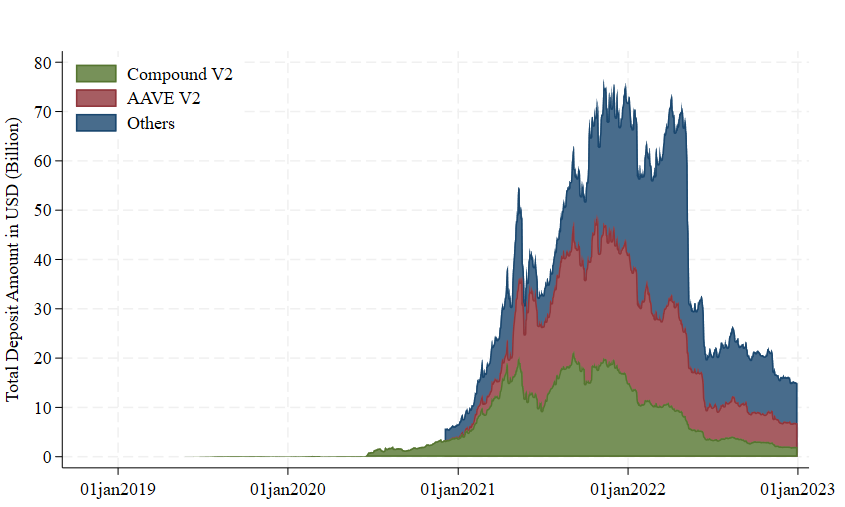
\includegraphics[width=0.95\linewidth]{figure/Deposit.png}}


\subfloat[Total Loan Amount in USD]{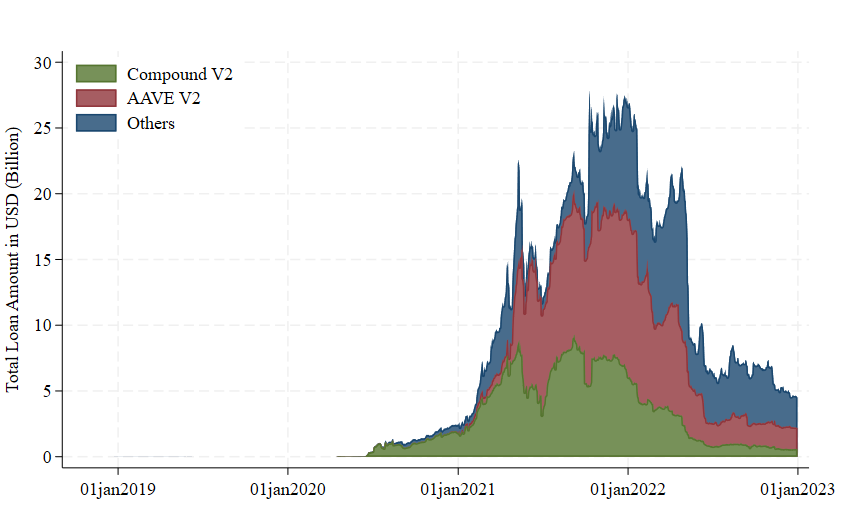
\includegraphics[width=0.95\linewidth]{figure/Loan.png}}

\end{figure}

\clearpage
\newpage
\begin{figure}[ht!]
\centering
\caption{Mechanisms of a Decentralized Financial Lending Platform}\label{fig:mechanism}
\caption*{This figure presents how AAVE facilitates borrowing and lending. The mechanisms are similar to those of Compound. Panel A provides an example of borrowing and lending, and Panel B presents positions after liquidation. }
\bigskip
\subfloat[Borrowing and Lending]{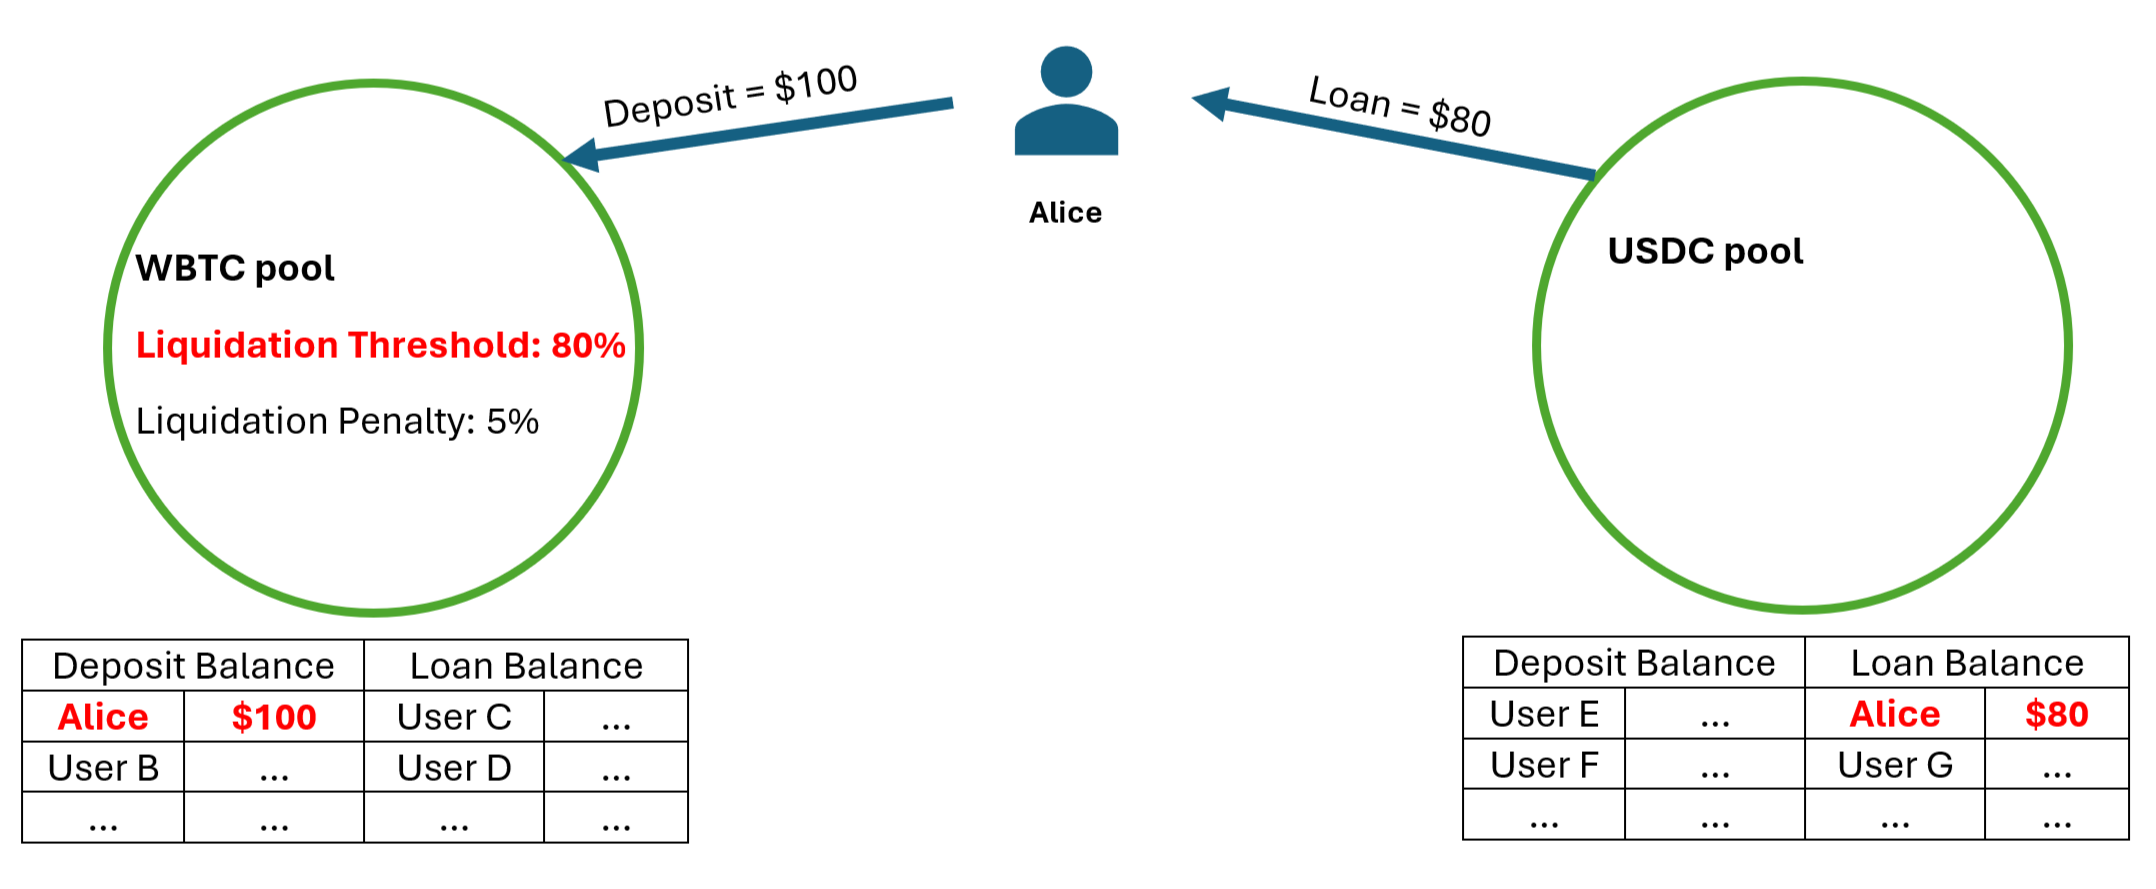
\includegraphics[width=\linewidth]{figure/mechanism1.png}}

\bigskip
\subfloat[Positions after Liquidation]{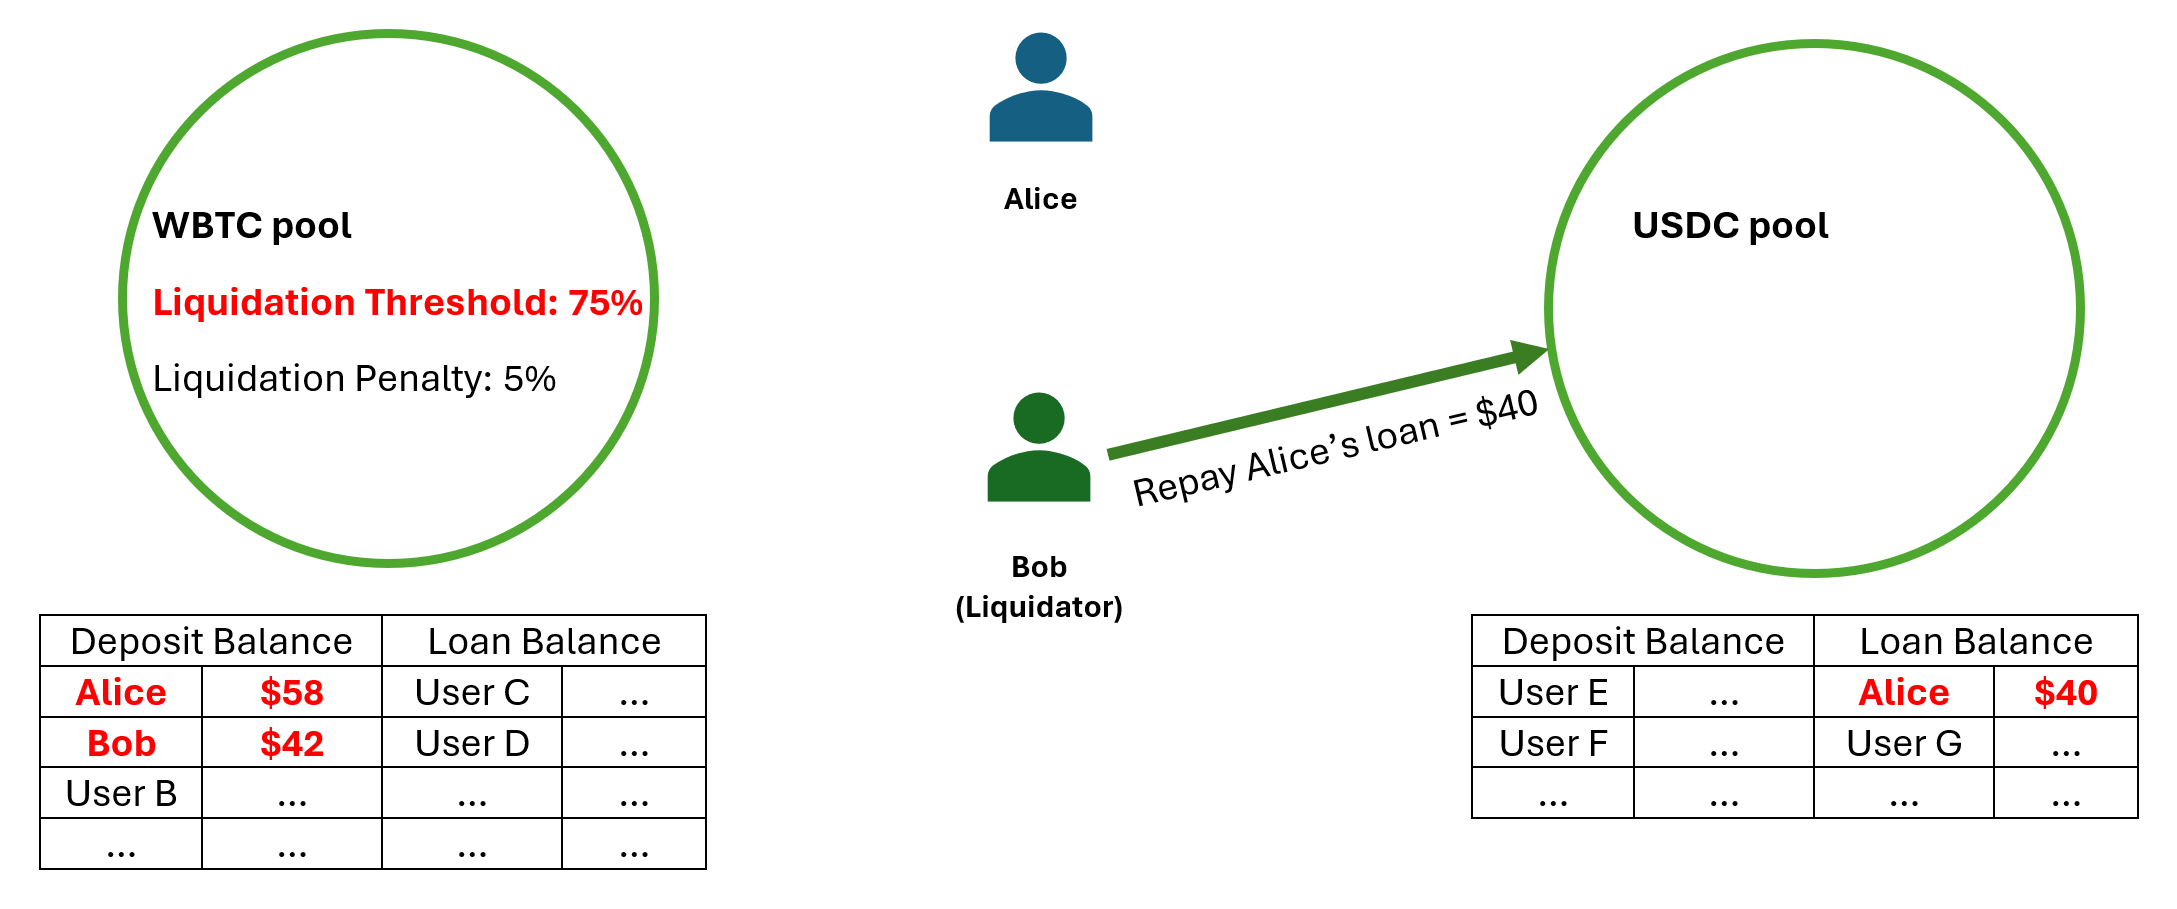
\includegraphics[width=\linewidth]{figure/mechanism2.png}}

\end{figure}

\clearpage
\newpage

\begin{figure}[ht!]
\centering
\caption{Governance Process}\label{fig:governance}
\caption*{This figure outlines the governance process within DeFi lending platforms. After creation, a proposal enters a discussion stage, allowing the community to evaluate its efficiency in a public forum. Following the discussion, the proposal advances to a voting stage. A successful proposal must obtain a majority of affirmative votes and exceed a predefined quorum number. If the proposal fails to meet these requirements, it will be rejected. The successful proposal then enters a timelock period, typically lasting one to two days, before execution. }
\subfloat{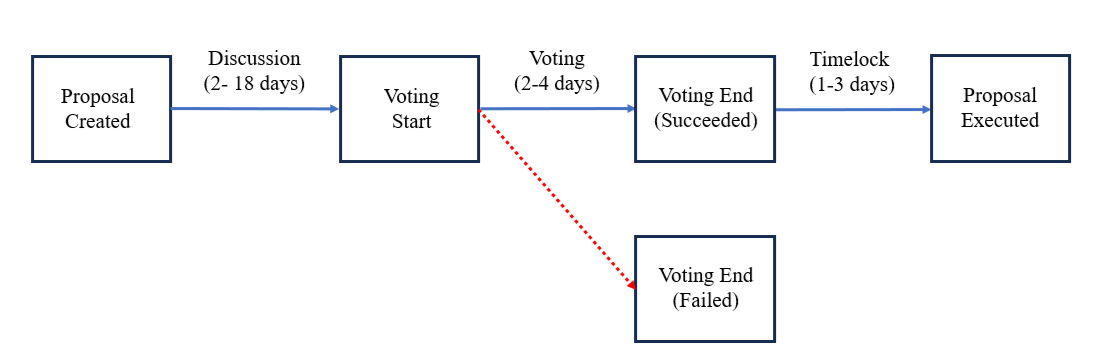
\includegraphics[width=\linewidth]{figure/voting.png}}

\end{figure}

\clearpage
\newpage


\begin{landscape}
\begin{figure}[ht!]
\centering
\caption{Deposits and Loans by Pools}\label{fig:deposit_loan_bypool}
\caption*{This figure plots the total deposit and loan amounts in US dollars of lending pools of USDC, DAI, WBTC, and WETH and other pools on AAVE and Compound from January 2021 to January 2023. The total deposit or total loan of all other pools is calculated by summing up the number of individual ones. }

\centering
\subfloat[Total Deposit Amount in USD on AAVE]{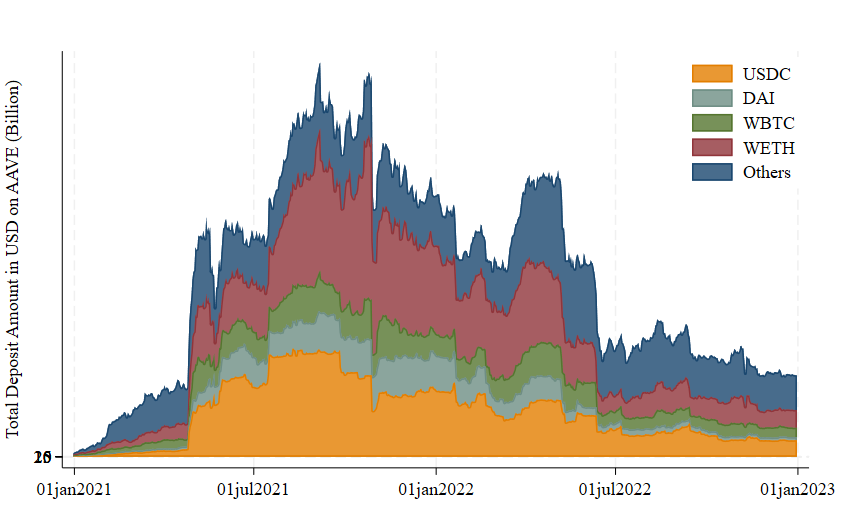
\includegraphics[width=0.48\linewidth]{figure/Deposit_AAVE_bypool.png}}
\subfloat[Total Loan Amount in USD on AAVE]{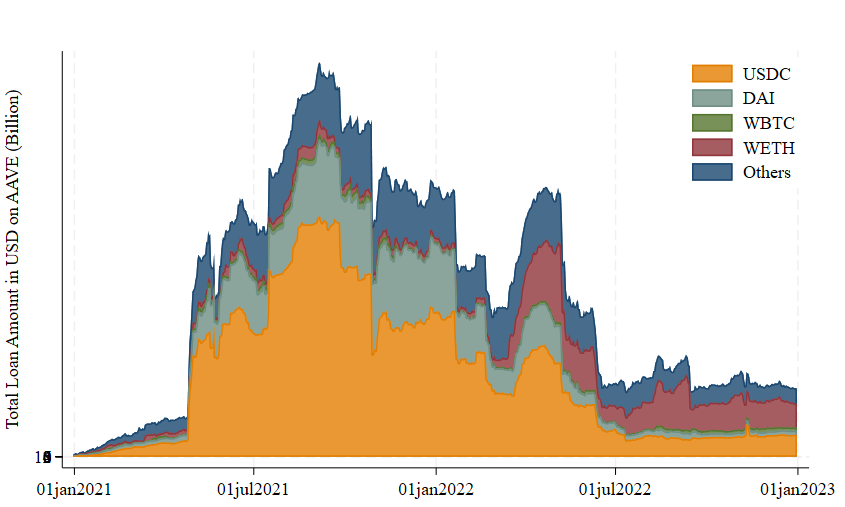
\includegraphics[width=0.48\linewidth]{figure/Loan_AAVE_bypool.png}}

\subfloat[Total Deposit Amount in USD on Compound]{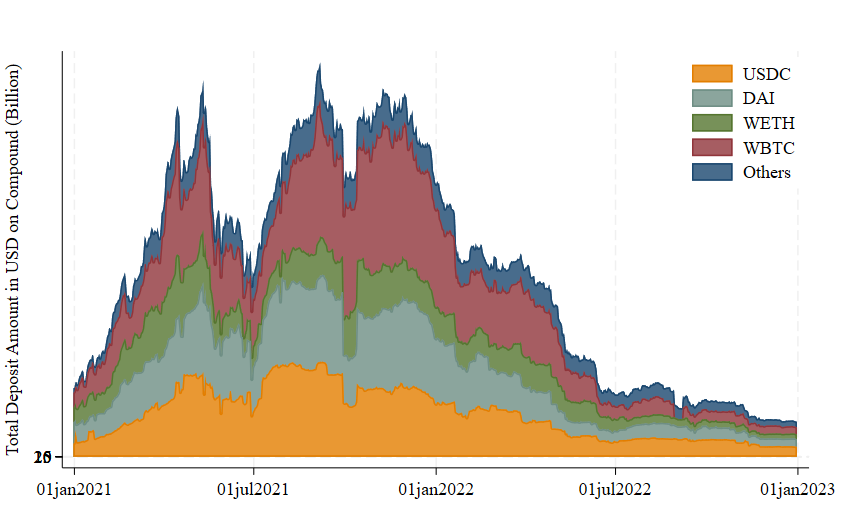
\includegraphics[width=0.48\linewidth]{figure/Deposit_COMP_bypool.png}}
\subfloat[Total Loan Amount in USD on Compound]{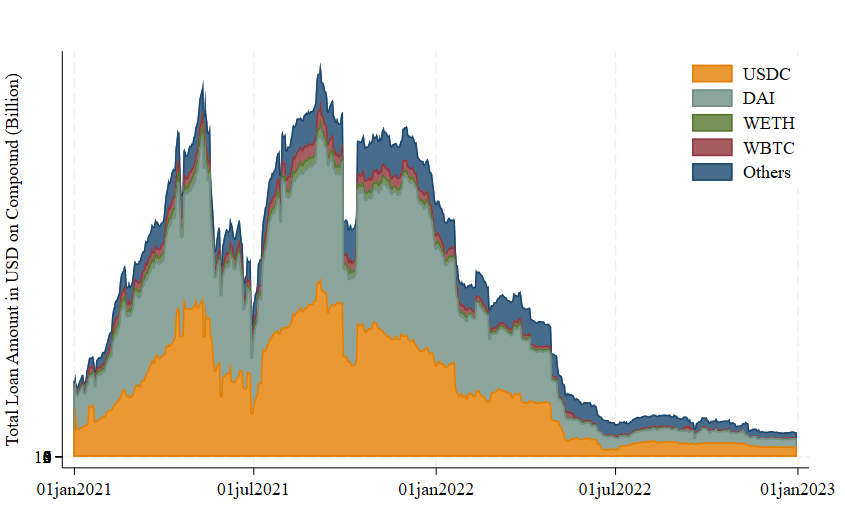
\includegraphics[width=0.48\linewidth]{figure/Loan_COMP_bypool.png}}

\end{figure}

\end{landscape}


\clearpage
\newpage


\begin{landscape}
\begin{figure}[ht!]
\centering
\caption{ Borrowing Rates}\label{fig:borrowingrate_major}
\caption*{This figure plots the borrowing rate of lending pools of USDC, DAI, WBTC, and WETH on AAVE and Compound and the Secured Overnight Financing Rate from January 2021 to January 2023.  }

\centering
\subfloat[USD Coin (USDC)]{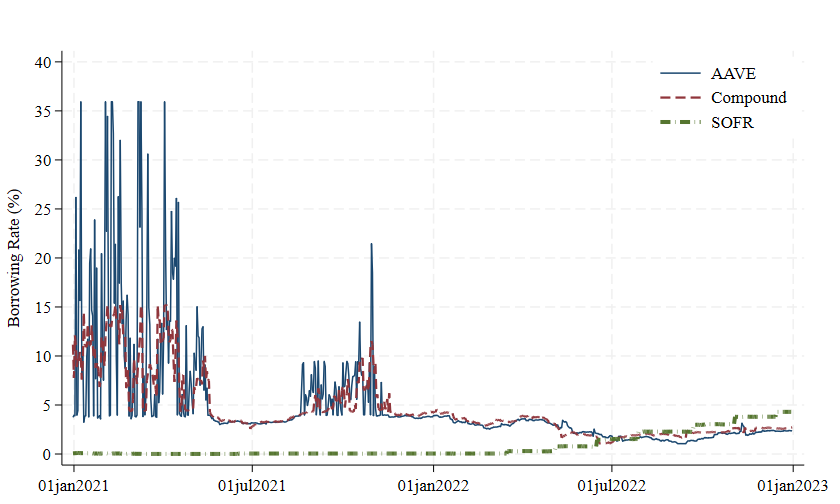
\includegraphics[width=0.48\linewidth]{figure/USDC_BRate.png}}
\subfloat[Dai (DAI)]{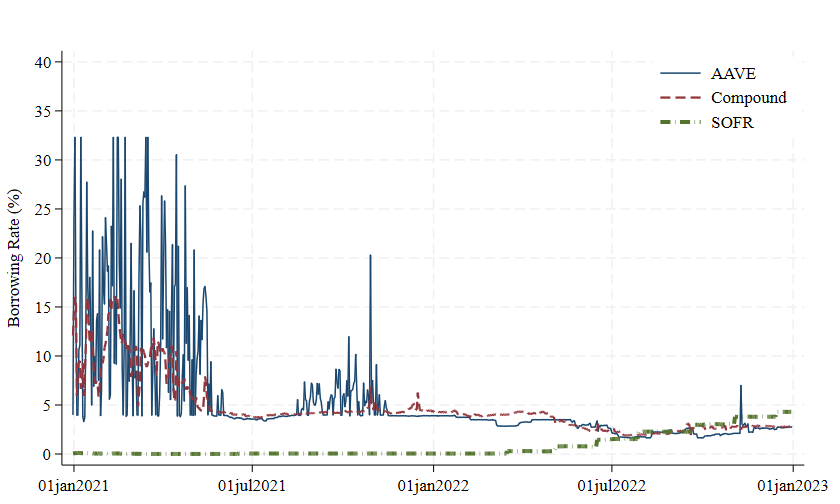
\includegraphics[width=0.48\linewidth]{figure/DAI_BRate.png}}

\subfloat[Wrapped Bitcoin (WBTC)]{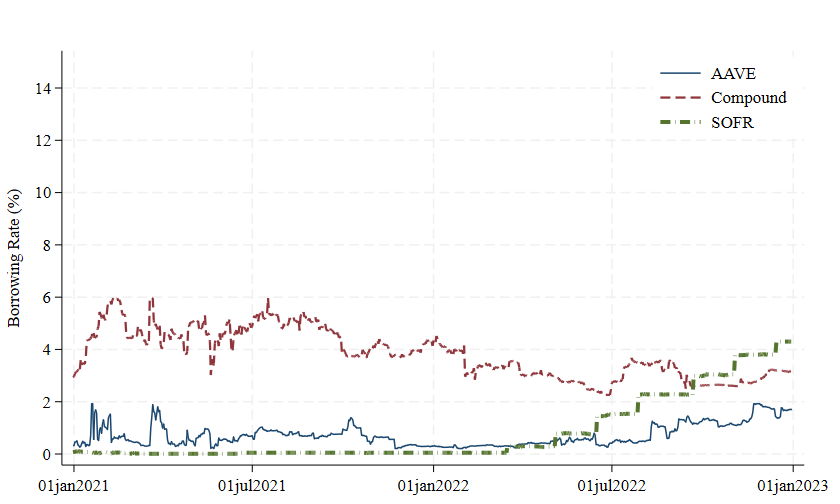
\includegraphics[width=0.48\linewidth]{figure/WBTC_BRate.png}}
\subfloat[Wrapped Ethereum (WETH)]{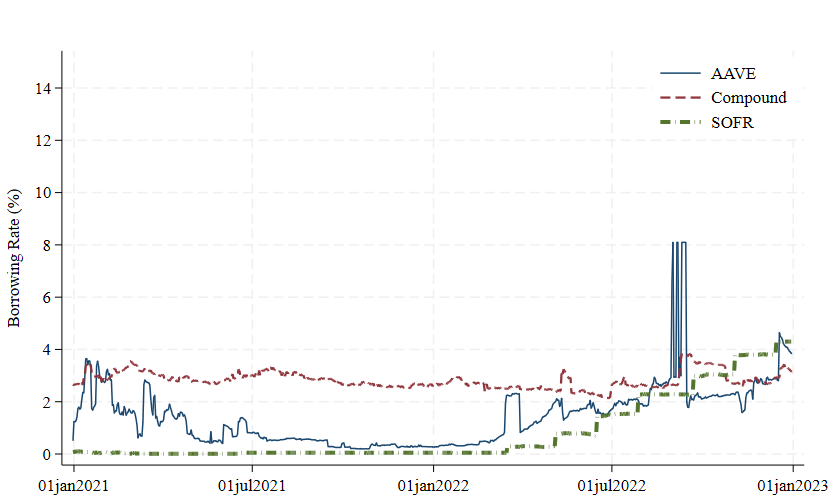
\includegraphics[width=0.48\linewidth]{figure/WETH_BRate.png}}

\end{figure}

\end{landscape}

\clearpage
\newpage
% \begin{landscape}
\begin{figure}[ht!]
\centering
\caption{Dynamics of Loan Balances}\label{fig:dynamics_borrow}
\caption*{This figure plots the estimations of $\beta$ coefficients from the Poisson pseudo-maximum likelihood regression: $TotalBorrow_{i,t}^p=\sum_{j=-7}^{7}\beta_jTreated_{i}^p\times I_j+\delta Treated_{i}^p+\sum_{s=-7}^{7}\sigma_sI_s+\textit{Borrower FE} + \textit{Collateral}\times\textit{Week FE}+\epsilon_{i,t}^p$, where $TotalBorrow_{i,t}^{p}$ represents the total loan balance in account $i$ on platform $p$ at the end of week $t$. $Treated_{i}^{p}$ is a binary variable that takes a value of 1 if account $i$ experiences a relaxation in margin requirements. $I_j$ is an indicator variable for weeks relative to the week of proposal execution. Standard errors are clustered at the borrower and week levels. The bars surrounding each coefficient represent the 5\% and 95\% confidence intervals.  }

\bigskip

% \subfloat[TotalBorrow (Dollar)]{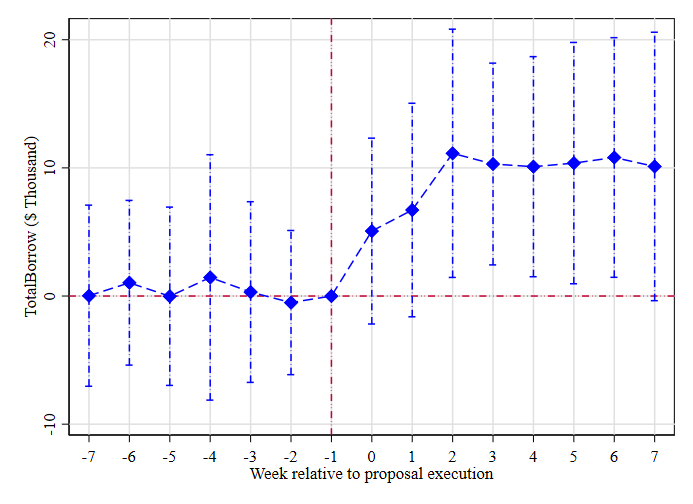
\includegraphics[width=0.45\linewidth]{figure/borrow_dollar.png}}
\subfloat{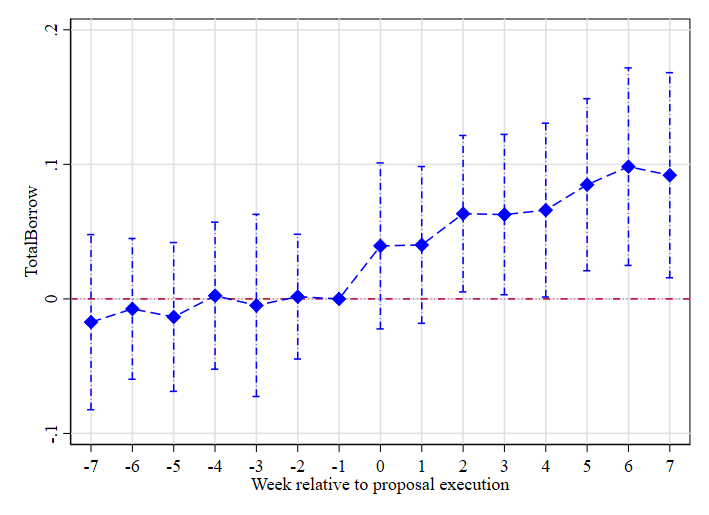
\includegraphics[width=\linewidth]{figure/borrow_pp.png}}
\end{figure}
% \end{landscape}

\clearpage
\newpage



% \begin{landscape}
\begin{figure}[ht!]
\centering
\caption{Dynamics of Deposit Balances}\label{fig:dynamics_deposit}
\caption*{This figure plots the estimations of $\beta$ coefficients from the Poisson pseudo-maximum likelihood regression: $Deposit_{i,t}^{c,p}=\sum_{j=-7}^{7}\beta_jTreated_{i}^p\times I_j+\delta Treated_{i}^p+\sum_{s=-7}^{7}\sigma_sI_s+\textit{Borrower FE} + \textit{Collateral}\times\textit{Week FE}+\epsilon_{i,t}^p$, where $Deposit_{i,t}^{c,p}$ represents the US dollar amount of the deposit balance in the treated or control pool of cryptocurrency $c$ on platform $p$ held by account $i$ at the end of week $t$. $Treated_{i}^{p}$ is a binary variable that takes a value of 1 if account $i$ experiences a relaxation in margin requirements. $I_j$ is an indicator variable for weeks relative to the week of proposal execution. Standard errors are clustered at the borrower and week levels. The bars surrounding each coefficient represent the 5\% and 95\% confidence intervals. }

\bigskip

% \subfloat[Deposit (Dollar)]{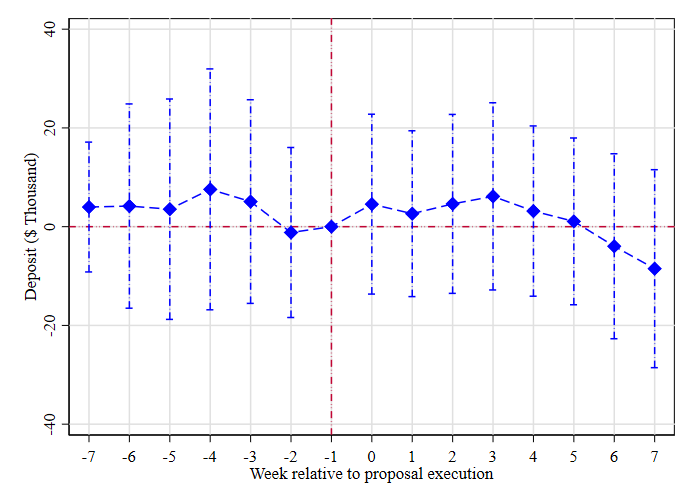
\includegraphics[width=0.45\linewidth]{figure/deposit_dollar.png}}
\subfloat{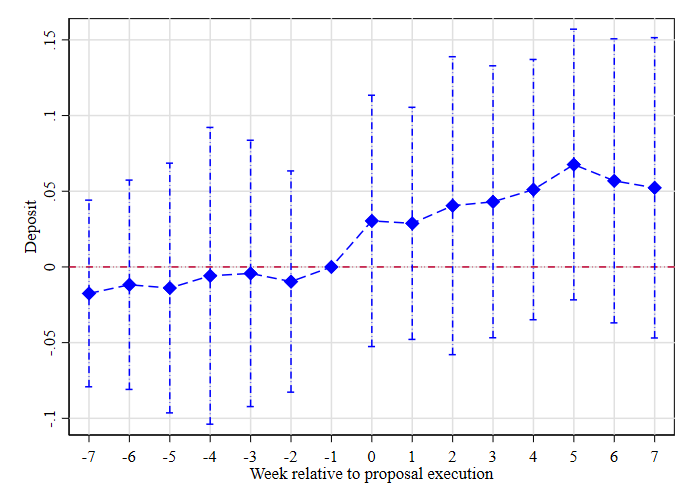
\includegraphics[width=\linewidth]{figure/deposit_pp.png}}

\end{figure}

% \end{landscape}

\clearpage
\newpage


\begin{landscape}
\begin{figure}[ht!]
\centering
\caption{Disproportionate Effects of Margin Requirements on Borrowers with Highly
Leveraged Positions}\label{fig:loandeposit_highlev}
\caption*{This figure repeats the analysis in Column (2) of Table \ref{tab:mainborrow} and Table \ref{tab:maindeposit} and plots the coefficient of $\beta_2$. Borrowers are sorted into quartiles based on the average leverage ratio, estimated using daily observations from the start of the event window to the day before the proposal discussion. Borrowers with the lowest leverage ratio are in the lowest quartile (Quartile 1). Borrowers with the highest leverage ratio are in the highest quartile (Quartile 4). The coefficient of $\beta_2$ for each quartile is presented. Standard errors are clustered at the borrower and week levels. The bars surrounding each coefficient represent the 5\% and 95\% confidence intervals. }

\bigskip

\subfloat[TotalBorrow]{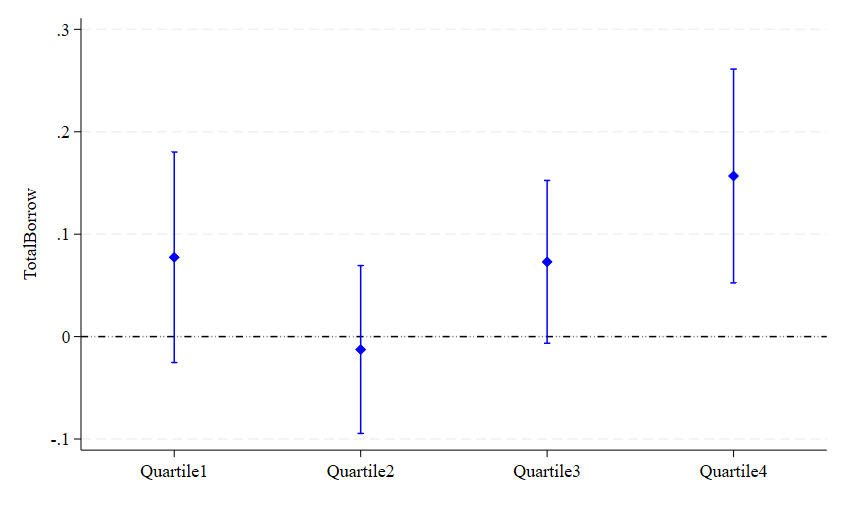
\includegraphics[width=0.45\linewidth]{figure/Heterogeneity/borrow.png}}
\subfloat[Deposit]{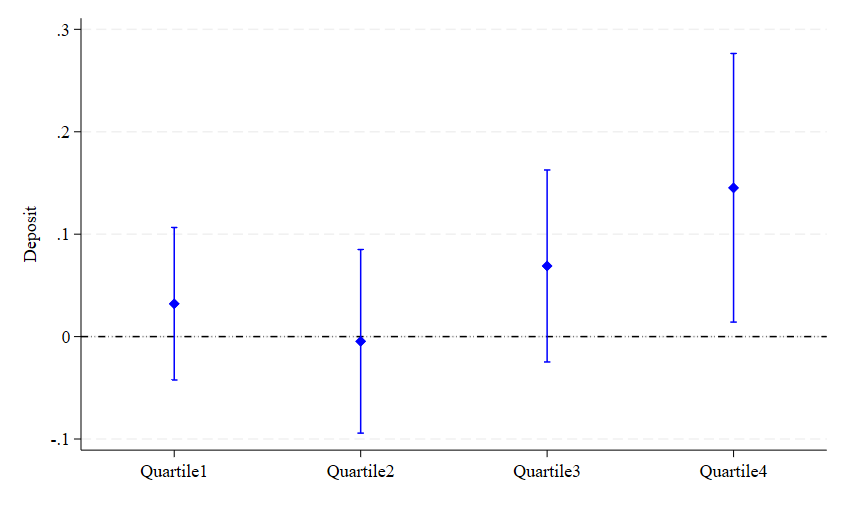
\includegraphics[width=0.45\linewidth]{figure/Heterogeneity/deposit.png}}
\end{figure}

\end{landscape}

\clearpage
\newpage


\begin{figure}[ht!]
\centering
\caption{Relaxed Margin Requirements and Leverage }\label{fig:post_lev}
\caption*{This figure repeats the same analysis in Column (2) of Table \ref{tab:mainborrow} and plots the coefficient of $\beta_2$. The dependent variable is $Leverage_{i,t}^p$, which represents the leverage of account $i$ on platform $p$ at the end of week $t$. The estimations are from the Ordinary Least Squares (OLS) regression model. Borrowers are sorted into quartiles based on the average leverage ratio, estimated using daily observations from the start of the event window to the day before the proposal discussion. Borrowers with the lowest leverage ratio are in the lowest quartile (Quartile 1). Borrowers with the highest leverage ratio are in the highest quartile (Quartile 4). The coefficient of $\beta_2$ for each quartile is presented. Standard errors are clustered at the borrower and week levels. The bars surrounding each coefficient represent the 5\% and 95\% confidence intervals. }

\subfloat{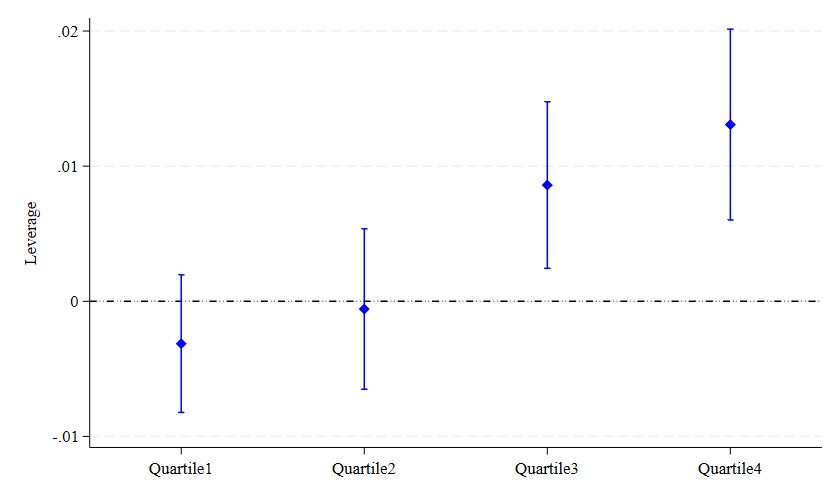
\includegraphics[width=\linewidth]{figure/Heterogeneity/lev.png}}
\end{figure}


\clearpage
\newpage


\begin{landscape}
\begin{figure}[ht!]
\centering
\caption{Dynamics of Leverage}\label{fig:dynamics_lev}
\caption*{This figure plots the estimations of $\beta$ coefficients from the Ordinary Least Squares regressions: $Leverage_{i,t}^{p}=\sum_{j=-7}^{7}\beta_jTreated_{i}^p\times I_j+\delta Treated_{i}^p+\sum_{s=-7}^{7}\sigma_sI_s+\textit{Borrower FE} + \textit{Collateral}\times\textit{Week FE}+\epsilon_{i,t}^p$, where $Leverage_{i,t}^{p}$ represents the leverage of account $i$ on platform $p$ at the end of week $t$. $Treated_{i}^{p}$ is a binary variable that takes a value of 1 if account $i$ experiences a relaxation in margin requirements. $I_j$ is an indicator variable for weeks relative to the week of proposal execution. Borrowers are sorted into quartiles based on the average leverage ratio, estimated using daily observations from the start of the event window to the day before the proposal discussion. Borrowers with the lowest leverage ratio are in the lowest quartile (Quartile 1). Borrowers with the highest leverage ratio are in the highest quartile (Quartile 4). Standard errors are clustered at the borrower and week levels. The bars surrounding each coefficient represent the 5\% and 95\% confidence intervals. }
\end{figure}

\end{landscape}

\clearpage
\newpage
\begin{landscape}
\begin{figure}[ht!]
\centering
\caption*{ Figure \ref{fig:dynamics_lev} - Continued from the previous page}
\subfloat[Quartile 1 (Lowest Leverage)]{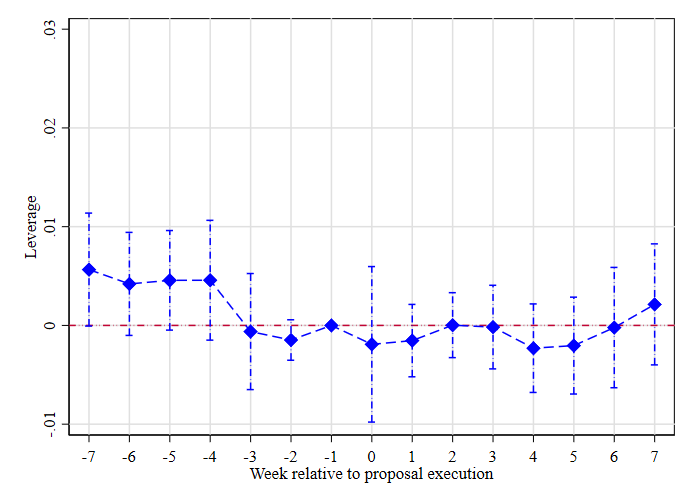
\includegraphics[width=0.45\linewidth]{figure/Heterogeneity/lev_g1.png}}
\subfloat[Quartile 2]{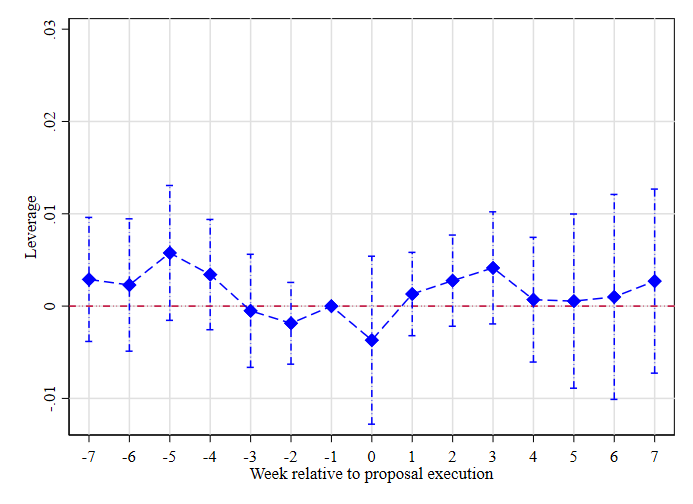
\includegraphics[width=0.45\linewidth]{figure/Heterogeneity/lev_g2.png}}

\subfloat[Quartile 3]{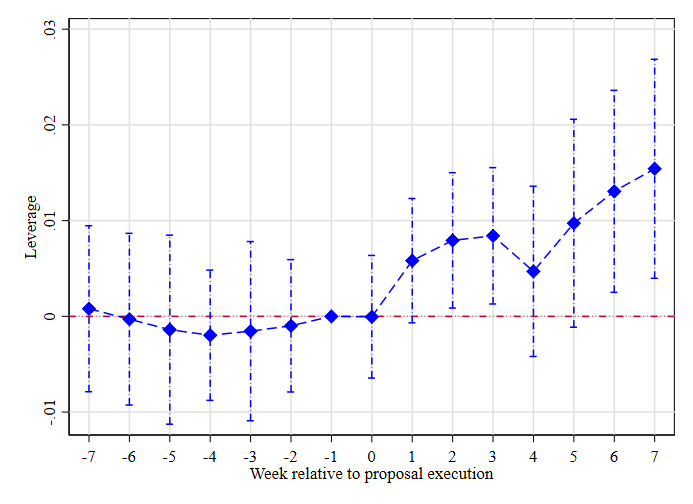
\includegraphics[width=0.45\linewidth]{figure/Heterogeneity/lev_g3.png}}
\subfloat[Quartile 4 (Highest Leverage)]{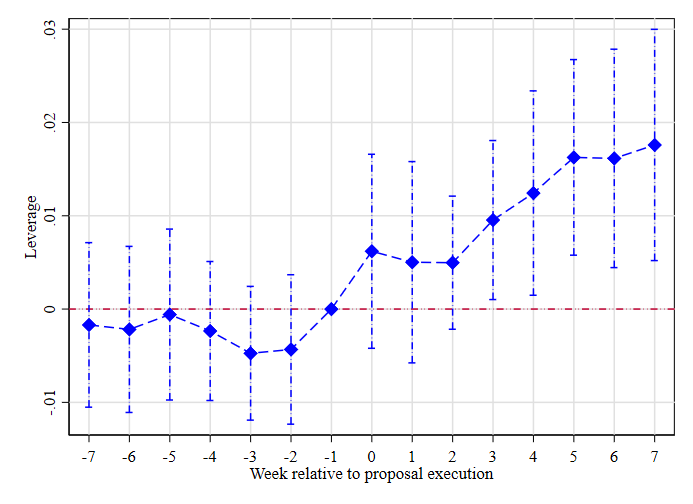
\includegraphics[width=0.45\linewidth]{figure/Heterogeneity/lev_g4.png}}

\end{figure}

\end{landscape}


\clearpage
\newpage



% \begin{landscape}
\begin{figure}[ht!]
\centering
\caption{Dynamics of Interest Rates of Stablecoins}\label{fig:dynamics_interestrates}
\caption*{This figure plots the estimations of $\beta$ coefficients from the OLS regression: $ Y_{c,t}^p=\sum_{j=-7}^{7}\beta_jTreated_{c}^p\times I_j+\delta Treated_{c}^p+\sum_{s=-7}^{7}\sigma_sI_s+ \textit{Crypto}\times\textit{Week FE}+\epsilon_{c,t}^p$, where $Y_{c,t}^p$ represents one of the utilization ratios, lending rates, and borrowing rates of cryptocurrency $c$ on platform $p$ at the end of week $t$. $Treated_{c}^{p}$ is a binary variable that takes a value of 1 if platform $p$, operating the cryptocurrency pool $c$, relaxes the margin requirements. $I_j$ is an indicator variable for weeks relative to the week of proposal execution. Standard errors are clustered at week levels. The bars surrounding each coefficient represent the 5\% and 95\% confidence intervals. }

\bigskip

% \subfloat[Deposit (Dollar)]{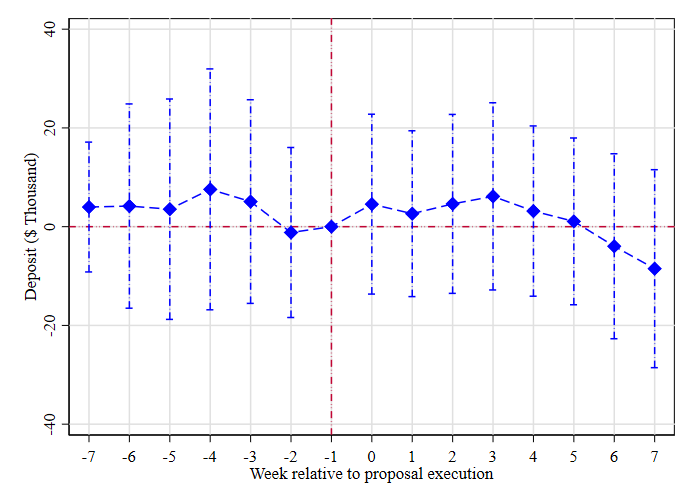
\includegraphics[width=0.45\linewidth]{figure/deposit_dollar.png}}
\subfloat[Utilization Ratio]{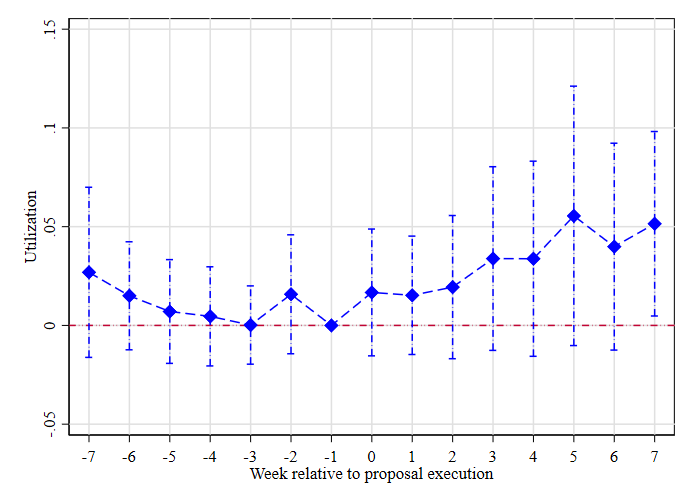
\includegraphics[width=\linewidth]{figure/Utilization.png}}

\end{figure}

% \end{landscape}

\clearpage
\newpage
\begin{figure}[ht!]
\ContinuedFloat 

\centering
\caption*{ Figure \ref{fig:dynamics_interestrates} - Continued from the previous page}
\subfloat[Lending Rate (\%)]{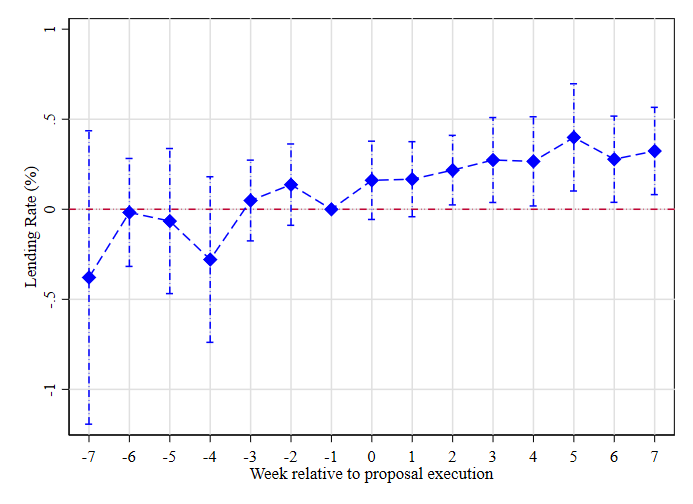
\includegraphics[width=0.85\linewidth]{figure/LendingRate.png}}

\subfloat[Borrowing Rate (\%)]{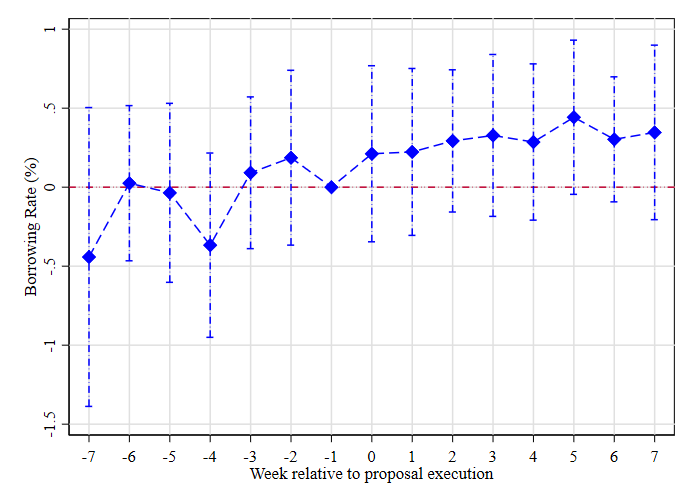
\includegraphics[width=0.85\linewidth]{figure/BorrowingRate.png}}

\end{figure}



%\documentclass[12pt]{article}
%\usepackage{times}
%\usepackage[round]{natbib}
%\usepackage{graphicx}
%\usepackage{tabularx, threeparttable, titling, comment, float}
%\usepackage{titling,amssymb,fullpage, multirow, microtype, booktabs, array,url,authblk,array,longtable,afterpage,pdflscape,booktabs, rotating, appendix}
%\usepackage[FIGTOPCAP]{subfigure}
%\usepackage{amsfonts,amsmath,amsthm, titlesec, hyperref, csquotes, adjustbox}
%\usepackage[usenames,dvipsnames,table]{xcolor}
%\usepackage[labelfont=bf,labelsep=colon,justification=justified]{caption}
%\usepackage[top=1in, bottom=1in, left=1in, right=1in]{geometry}
%\usepackage{setspace}
%\usepackage{enumitem}
%\usepackage{siunitx} % better
%%
%%
%%
%\titlespacing{\section}{0pt}{*0}{*0}
%\titlespacing{\subsection}{0pt}{*0}{*0}
%\titlespacing{\subsubsection}{0pt}{*0}{*0}
%%
%\setlength{\parskip}{1mm}
%\setlength{\widowpenalty}{10000}          %/*150*/ No Widows at bottom of page
%\setlength{\displaywidowpenalty}{10000}   %/*50*/
%\setlength{\clubpenalty}{100000}          % No orphans at top of page
%\setlist[itemize]{topsep=0pt}
%%
%\renewcommand*{\thesubfigure}{\Alph{subfigure})}
%\setlength{\abovedisplayskip}{0pt}
%\setlength{\belowdisplayskip}{0pt}
%\setlength{\abovedisplayshortskip}{0pt}
%\setlength{\belowdisplayshortskip}{0pt}
%
%
%%\usepackage{xr}
%%\externaldocument{Internet_Appendix}
%
%\begin{document}


%% Tables

\clearpage
\newpage
%\setlength{\tabcolsep}{1pt}
        

\begin{table}[ht!]
%\footnotesize 
\caption{Summary Statistics of Deposits and Loans}\label{tab:pool_sumstat_DL}
\caption*{This table presents summary statistics of the total deposit and loan amounts in US dollars on pool-day level data. The sample includes lending pools of USDC, DAI, WBTC, and WETH and pools other than those four on AAVE and Compound from January 2021 to January 2023. The total deposit or total loan of all other pools is calculated by summing up the number of individual ones. All variables are winsorized at the $1^{st}$ and $99^{th}$ percentiles.}


\centering
\def\sym#1{\ifmmode^{#1}\else\(^{#1}\)\fi}


\begin{tabular*}{\linewidth}{@{\extracolsep{\fill}}lccccccc}

    \toprule
    Variable  & N & Mean & SD & P25 & Median & P75 \\
    \midrule
    \multicolumn{7}{c}{Panel A: Deposit (\$, Billion)} \\
    \midrule
    AAVE-USDC  & 731   & 2.48  & 1.72  & 0.99  & 2.32  & 3.62 \\[2pt]
    AAVE-DAI  & 731   & 0.91  & 0.73  & 0.20  & 0.74  & 1.61 \\[2pt]
    AAVE-WBTC  & 731   & 1.09  & 0.57  & 0.61  & 1.14  & 1.50 \\[2pt]
    AAVE-WETH  & 731   & 2.85  & 2.11  & 1.00  & 2.37  & 4.39 \\[2pt]
    AAVE-Others  & 731   & 2.73  & 0.99  & 2.21  & 2.68  & 3.28 \\[2pt]
    COMP-USDC  & 731   & 2.40  & 1.40  & 1.00  & 2.43  & 3.58 \\[2pt]
    COMP-DAI  & 731   & 2.30  & 1.48  & 0.74  & 2.30  & 3.62 \\[2pt]
    COMP-WBTC  & 731   & 1.38  & 0.77  & 0.69  & 1.36  & 1.91 \\[2pt]
    COMP-WETH  & 731   & 2.99  & 2.13  & 0.87  & 2.75  & 4.69 \\[2pt]
    COMP-Others  & 731   & 1.13  & 0.48  & 0.70  & 1.25  & 1.52 \\
    \midrule
    \multicolumn{7}{c}{Panel B: Loan (\$, Billion)} \\
    \midrule
    AAVE-USDC  & 731   & 1.84  & 1.56  & 0.44  & 1.44  & 2.98 \\[2pt]
    AAVE-DAI  & 731   & 0.66  & 0.59  & 0.10  & 0.54  & 1.18 \\[2pt]
    AAVE-WBTC  & 731   & 0.06  & 0.03  & 0.03  & 0.06  & 0.08 \\[2pt]
    AAVE-WETH  & 731   & 0.39  & 0.37  & 0.12  & 0.20  & 0.61 \\[2pt]
    AAVE-Others  & 731   & 0.77  & 0.41  & 0.40  & 0.83  & 1.15 \\[2pt]
    COMP-USDC  & 731   & 1.63  & 1.16  & 0.37  & 1.50  & 2.65 \\[2pt]
    COMP-DAI  & 731   & 1.70  & 1.22  & 0.32  & 1.82  & 2.84 \\[2pt]
    COMP-WBTC  & 731   & 0.09  & 0.07  & 0.02  & 0.08  & 0.15 \\[2pt]
    COMP-WETH  & 731   & 0.14  & 0.10  & 0.04  & 0.14  & 0.23 \\[2pt]
    COMP-Others  & 731   & 0.48  & 0.22  & 0.27  & 0.51  & 0.66 \\
    \bottomrule

          \end{tabular*} 



\end{table}%

\clearpage
\newpage
%\setlength{\tabcolsep}{1pt}
        

\begin{table}[ht!]
%\footnotesize 
\caption{Summary Statistics of Borrowing and Lending Rates}\label{tab:pool_sumstat_I}
\caption*{This table presents summary statistics of borrowing and lending rates in percentage on pool-day level data and the Secured Overnight Financing Rate (SOFR) in percentage. The sample includes lending pools of USDC, DAI, WBTC, and WETH and pools other than those four on AAVE and Compound from January 2021 to December 2023. The borrowing (lending) rates of all other pools are the loan (deposit) amount weighted average of individual ones. All variables are winsorized at the $1^{st}$ and $99^{th}$ percentiles.}


\centering
\def\sym#1{\ifmmode^{#1}\else\(^{#1}\)\fi}


\begin{tabular*}{\linewidth}{@{\extracolsep{\fill}}lccccccc}

    \toprule
    Variable  & N & Mean & SD & P25 & Median & P75 \\
    \midrule
    \multicolumn{7}{c}{Panel A: Lending Rate (\%)} \\
    \midrule
    AAVE-USDC  & 731   & 3.46  & 3.47  & 1.08  & 2.26  & 4.59 \\[2pt]
    AAVE-DAI  & 731   & 3.43  & 3.09  & 1.39  & 2.49  & 3.92 \\[2pt]
    AAVE-WBTC  & 731   & 0.05  & 0.05  & 0.01  & 0.03  & 0.07 \\[2pt]
    AAVE-WETH  & 731   & 0.53  & 0.81  & 0.02  & 0.19  & 0.77 \\[2pt]
    AAVE-Others  & 731   & 1.58  & 1.43  & 0.73  & 1.23  & 1.68 \\[2pt]
    COMP-USDC  & 731   & 2.99  & 2.84  & 0.84  & 2.00  & 3.31 \\[2pt]
    COMP-DAI  & 731   & 2.91  & 2.32  & 1.12  & 2.56  & 2.96 \\[2pt]
    COMP-WBTC  & 731   & 0.19  & 0.14  & 0.07  & 0.17  & 0.27 \\[2pt]
    COMP-WETH  & 731   & 0.12  & 0.06  & 0.07  & 0.09  & 0.16 \\[2pt]
    COMP-Others  & 731   & 2.08  & 1.39  & 1.26  & 1.57  & 2.13 \\
    \midrule
    \multicolumn{7}{c}{Panel B: Borrowing Rate (\%)} \\
    \midrule
    AAVE-USDC  & 731   & 5.01  & 5.71  & 2.27  & 3.30  & 3.97 \\[2pt]
    AAVE-DAI  & 731   & 5.44  & 5.61  & 2.75  & 3.66  & 4.40 \\[2pt]
    AAVE-WBTC  & 731   & 0.71  & 0.42  & 0.37  & 0.58  & 0.96 \\[2pt]
    AAVE-WETH  & 731   & 1.45  & 1.21  & 0.49  & 1.36  & 2.11 \\[2pt]
    AAVE-Others  & 731   & 7.17  & 6.05  & 3.86  & 4.48  & 7.41 \\[2pt]
    COMP-USDC  & 731   & 4.53  & 3.16  & 2.34  & 3.48  & 4.54 \\[2pt]
    COMP-DAI  & 731   & 4.67  & 2.80  & 2.83  & 4.09  & 4.41 \\[2pt]
    COMP-WBTC  & 731   & 3.83  & 0.93  & 3.03  & 3.74  & 4.59 \\[2pt]
    COMP-WETH  & 731   & 2.82  & 0.32  & 2.60  & 2.75  & 3.00 \\[2pt]
    COMP-Others  & 731   & 5.30  & 3.19  & 3.39  & 4.10  & 5.24 \\[2pt]
    SOFR  & 500   & 0.83  & 1.28  & 0.05  & 0.05  & 1.52 \\
    \bottomrule

          \end{tabular*} 



\end{table}%
    
\clearpage
\newpage
\begin{landscape}
    

\begin{table}[htbp]
%\footnotesize 

  \caption{Governance Proposals}\label{tab:proposals}
  
\caption*{This table presents the timelines for each proposal, including the start of the discussion period, the start and end of the voting period, and the date of execution. The Proposal ID includes the name of the DeFi lending platform, indicating whether AAVE or Compound (COMP) initiated this proposal. }

\def\sym#1{\ifmmode^{#1}\else\(^{#1}\)\fi}


   \begin{tabular*}{\linewidth}{@{\extracolsep{\fill}}ccccc}
    \toprule
    Proposal & Discussion & Voting & Voting & Execution \\
      ID        &   Begin    & Begin & End &  \\
    \midrule
    %   \multicolumn{12}{c}{Panel A: Proposals to decrease collateral requirements} \\
    % \midrule
      % AAVE-39 & WETH  & 0.800 & 0.825 &       &       &       &       & 9/30/2021 & 10/5/2021 & 10/8/2021 & 10/9/2021 \\
    % AAVE-39 & YFI   & 0.450 & 0.500 & 0.600 & 0.650 &       &       & 9/30/2021 & 10/5/2021 & 10/8/2021 & 10/9/2021 \\
    % AAVE-39 & ZRX   & 0.600 & 0.650 & 0.700 & 0.750 &       &       & 9/30/2021 & 10/5/2021 & 10/8/2021 & 10/9/2021 \\
    % AAVE-40 & BAT   &       &       & 0.750 & 0.800 &       &       & 10/8/2021 & 10/11/2021 & 10/14/2021 & 10/15/2021 \\
    % AAVE-42 & UNI   & 0.550 & 0.600 &       &       &       &       & 10/15/2021 & 10/18/2021 & 10/21/2021 & 10/22/2021 \\
    % AAVE-53 & BAT   & 0.700 & 0.750 &       &       &       &       & 12/16/2021 & 12/21/2021 & 12/24/2021 & 12/25/2021 \\
    % AAVE-53 & ZRX   & 0.600 & 0.650 &       &       &       &       & 12/16/2021 & 12/21/2021 & 12/24/2021 & 12/25/2021 \\
    % AAVE-58 & FEI   & 0.500 & 0.600 & 0.600 & 0.700 &       &       & 2/11/2022 & 2/16/2022 & 2/19/2022 & 2/20/2022 \\
    % AAVE-67 & FEI   & 0.600 & 0.650 & 0.700 & 0.750 &       &       & 3/18/2022 & 3/23/2022 & 3/26/2022 & 3/27/2022 \\
     % AAVE-69 & DAI   & 0.750 & 0.770 &       &       &       &       & 4/1/2022 & 4/5/2022 & 4/8/2022 & 4/9/2022 \\
    % AAVE-69 & LINK  &       &       & 0.750 & 0.780 &       &       & 4/1/2022 & 4/5/2022 & 4/8/2022 & 4/9/2022 \\
    AAVE-69     & 4/1/2022 & 4/5/2022 & 4/8/2022 & 4/9/2022 \\[2pt]
    % AAVE-70 & UNI   &       &       & 0.700 & 0.750 &       &       & 4/22/2022 & 4/26/2022 & 4/29/2022 & 5/1/2022 \\
     AAVE-92      & 8/4/2022 & 8/9/2022 & 8/13/2022 & 8/14/2022 \\[2pt]
    % AAVE-92 & LINK  &       &       & 0.780 & 0.830 &       &       & 8/4/2022 & 8/9/2022 & 8/13/2022 & 8/14/2022 \\
    AAVE-94         & 8/18/2022 & 8/23/2022 & 8/27/2022 & 8/28/2022 \\[2pt]
    AAVE-102       & 9/23/2022 & 9/27/2022 & 9/30/2022 & 10/1/2022 \\[2pt]
    % AAVE-102 & UNI   & 0.600 & 0.650 & 0.750 & 0.770 &       &       & 9/23/2022 & 9/27/2022 & 9/30/2022 & 10/1/2022 \\
    AAVE-108       & 10/7/2022 & 10/12/2022 & 10/14/2022 & 10/15/2022 \\[2pt]
       COMP-36       & 1/15/2021 & 2/2/2021 & 2/4/2021 & 2/6/2021 \\[2pt]
    % Compound-39 & ZRX   &       &       &       &       & 0.600 & 0.650 & 2/20/2021 & 3/3/2021 & 3/5/2021 & 3/7/2021 \\
    % Compound-39 & BAT   &       &       &       &       & 0.600 & 0.650 & 2/20/2021 & 3/3/2021 & 3/5/2021 & 3/7/2021 \\
    % Compound-66 & LINK  &       &       &       &       & 0.500 & 0.600 & 10/25/2021 & 11/3/2021 & 11/7/2021 & 11/9/2021 \\
    % Compound-66 & MKR   &       &       &       &       & 0.350 & 0.450 & 10/25/2021 & 11/3/2021 & 11/7/2021 & 11/9/2021 \\
    COMP-66       & 10/25/2021 & 11/3/2021 & 11/7/2021 & 11/9/2021 \\[2pt]
    % Compound-66 & YFI   &       &       &       &       & 0.350 & 0.550 & 10/25/2021 & 11/3/2021 & 11/7/2021 & 11/9/2021 \\
     COMP-71      & 11/18/2021 & 11/21/2021 & 11/25/2021 & 11/28/2021 \\[2pt]
    % Compound-72 & UNI   &       &       &       &       & 0.600 & 0.700 & 11/30/2021 & 12/3/2021 & 12/6/2021 & 12/8/2021 \\
    COMP-74   & 12/12/2021 & 12/14/2021 & 12/17/2021 & 12/20/2021 \\[2pt]
    % Compound-74 & BAT   &       &       &       &       & 0.600 & 0.650 & 12/12/2021 & 12/14/2021 & 12/17/2021 & 12/20/2021 \\
    % Compound-74 & LINK  &       &       &       &       & 0.650 & 0.700 & 12/12/2021 & 12/14/2021 & 12/17/2021 & 12/20/2021 \\
     COMP-81       & 1/7/2022 & 1/13/2022 & 1/16/2022 & 1/18/2022 \\
    % Compound-85 & UNI   &       &       &       &       & 0.700 & 0.750 & 2/12/2022 & 2/21/2022 & 2/25/2022 & 2/28/2022 \\
    % Compound-85 & LINK  &       &       &       &       & 0.700 & 0.750 & 2/12/2022 & 2/21/2022 & 2/25/2022 & 2/28/2022 \\
    % Compound-85 & MKR   &       &       &       &       & 0.550 & 0.600 & 2/12/2022 & 2/21/2022 & 2/25/2022 & 2/28/2022 \\
    % Compound-85 & YFI   &       &       &       &       & 0.600 & 0.650 & 2/12/2022 & 2/21/2022 & 2/25/2022 & 2/28/2022 \\
    % Compound-90 & ZRX   &       &       &       &       & 0.600 & 0.650 & 3/10/2022 & 3/16/2022 & 3/19/2022 & 3/21/2022 \\
    % Compound-90 & MKR   &       &       &       &       & 0.600 & 0.650 & 3/10/2022 & 3/16/2022 & 3/19/2022 & 3/21/2022 \\
    % Compound-98 & YFI   &       &       &       &       & 0.650 & 0.700 & 3/29/2022 & 4/6/2022 & 4/9/2022 & 4/11/2022 \\
    % Compound-103 & MKR   &       &       &       &       & 0.650 & 0.700 & 4/20/2022 & 4/27/2022 & 4/30/2022 & 5/2/2022 \\
    % Compound-107 & USDC        &       &       & 0.800 & 0.825 & 5/19/2022 & 5/25/2022 & 5/28/2022 & 5/31/2022 \\
    %  Compound-107 & DAI         &       &       & 0.800 & 0.825 & 5/19/2022 & 5/25/2022 & 5/28/2022 & 5/31/2022 \\
    % Compound-107 & MKR   &       &       &       &       & 0.700 & 0.730 & 5/19/2022 & 5/25/2022 & 5/28/2022 & 5/31/2022 \\
    % Compound-107 & LINK  &       &       &       &       & 0.750 & 0.770 & 5/19/2022 & 5/25/2022 & 5/28/2022 & 5/31/2022 \\
    % Compound-107 & YFI   &       &       &       &       & 0.700 & 0.730 & 5/19/2022 & 5/25/2022 & 5/28/2022 & 5/31/2022 \\
    % \midrule
    %     \multicolumn{12}{c}{Panel B: Proposals to increase collateral requirements} \\
    % \midrule
    % AAVE-39 & UNI   & 0.600 & 0.550 &       &       &       &       & 9/30/2021 & 10/5/2021 & 10/8/2021 & 10/9/2021 \\ [2pt]
    % AAVE-43 & ZRX   & 0.650 & 0.600 &       &       &       &       & 10/21/2021 & 10/25/2021 & 10/28/2021 & 10/29/2021 \\[2pt]
    % AAVE-137 & DAI   & 0.770 & 0.750 & 0.900 & 0.870 &       &       & 12/1/2022 & 12/21/2022 & 12/24/2022 & 12/25/2022 \\[2pt]
    % AAVE-137 & USDC  & 0.870 & 0.800 & 0.890 & 0.875 &       &       & 12/1/2022 & 12/21/2022 & 12/24/2022 & 12/25/2022 \\[2pt]
    % Compound-39 & WBTC  &       &       &       &       & 0.750 & 0.650 & 2/6/2021 & 3/3/2021 & 3/5/2021 & 3/7/2021 \\[2pt]   
    \bottomrule
            % \\ \multicolumn{12}{r}{\textit{(continued on next page)}}\\
    
\end{tabular*} 
\end{table}
\end{landscape}


\clearpage
\newpage
%\setlength{\tabcolsep}{1pt}
    \begin{landscape}
        

\begin{table}[ht!]
%\footnotesize 
\caption{Margin Requirements for the Treated and Control Pools}\label{tab:proposal_margin}
\caption*{This table lists margin requirements for each treated pool and control pool. The Liquidation Threshold (LT) and the Collateral Factor (CF) regulate margin requirements on AAVE and Compound, respectively. AAVE (Compound) assigns the Liquidation Threshold (Collateral Factor) to each lending pool. The Liquidation Threshold or the Collateral Factor of a lending pool determines the maximum loan amount an account can have to prevent liquidation if the account uses \$1 of deposits in this lending pool as collateral. The Proposal ID and lending pool include the name of the DeFi lending platform.}


\centering
\def\sym#1{\ifmmode^{#1}\else\(^{#1}\)\fi}


\begin{tabular*}{\linewidth}{@{\extracolsep{\fill}}llcclc}
    \toprule
    Proposal & Treated Pool & LT/CF (\%)  & LT/CF (\%) & Control Pool & LT/CF (\%) \\
     ID &   &   From &   To & &  \\
          &       & (Treated Pool) & (Treated Pool)&  & (Control Pool) \\
          \midrule
    AAVE-69 & AAVE-USDC & 85.0 & 86.0 & COMP-USDC& 80.0 \\[2pt]
    AAVE-92 & AAVE-DAI & 80.0 & 85.0& COMP-DAI & 83.5 \\[2pt]
    AAVE-94 & AAVE-WBTC & 75.0 & 80.0 & COMP-WBTC& 70.0 \\[2pt]
    AAVE-102 & AAVE-USDC & 88.0 & 89.0& COMP-USDC & 85.5 \\[2pt]
    AAVE-102 & AAVE-WETH & 85.0 & 86.0& COMP-WETH & 82.5 \\[2pt]
    AAVE-108 & AAVE-WBTC & 80.0 & 82.0& COMP-WBTC & 70.0 \\[2pt]
    COMP-36 & COMP-WBTC & 60.0 & 75.0 & AAVE-WBTC& 75.0 \\[2pt]
    COMP-66 & COMP-USDC & 75.0 & 80.0 & AAVE-USDC& 85.0 \\[2pt]
    COMP-71 & COMP-DAI & 75.0 & 80.0 & AAVE-DAI& 80.0 \\[2pt]
    COMP-71 & COMP-WETH & 75.0 & 80.0 & AAVE-WETH& 85.0 \\[2pt]
    COMP-74 & COMP-WBTC & 65.0 & 70.0 & AAVE-WBTC& 75.0 \\[2pt]
    COMP-81 & COMP-WETH & 80.0 & 82.5 & AAVE-WETH & 85.0 \\
    \midrule

          \end{tabular*} 



\end{table}%
    \end{landscape}

\clearpage
\newpage
%\setlength{\tabcolsep}{1pt}
        

\begin{table}[ht!]
\caption{Summary Statistics of Margin Requirements}\label{tab:proposal_sumstat}
\caption*{This table provides summary statistics of margin requirements for the treated and control pools. The Liquidation Threshold and the Collateral Factor regulate the margin requirements on AAVE and Compound, respectively. AAVE (Compound) assigns the Liquidation Threshold (Collateral Factor) to each lending pool, and this risk parameter determines the maximum loan amount an account can have to prevent liquidation if the account uses \$1 of deposits in this lending pool as collateral. }


\centering
\def\sym#1{\ifmmode^{#1}\else\(^{#1}\)\fi}


\begin{tabular*}{\linewidth}{@{\extracolsep{\fill}}lccc}
    \toprule
     &   LT/CF (\%)  & LT/CF (\%)  & LT/CF (\%) \\
          &   From &  To &\\
               & (Treated Pool)  & (Treated Pool)  &  (Control Pool) \\
          \midrule
    Mean        & 76.9   & 81.3   & 79.7 \\
    SD           & 8.1   & 5.2  &  5.8 \\
    P25        & 75.0   & 80.0   & 75.0 \\
    Median       & 77.5   & 81.0   & 81.3 \\
    P75         & 81.3   & 85.3  &  85.0 \\
    \bottomrule
          \end{tabular*} 



\end{table}%
    
\clearpage
\newpage
%\setlength{\tabcolsep}{1pt}
    

\begin{table}[ht!]
%\footnotesize 
\caption{Summary Statistics of Borrowing and Lending Positions}\label{tab:sumstat}
\caption*{This table presents summary statistics of borrowing and lending positions. $Deposit$ is the US dollar amount (in thousands) of the deposit balance in the treated or control pool. $TotalDeposit$ is the aggregated deposit balance in thousands, calculated by summing the US dollar amounts across all lending positions on the platform. $TotalBorrow$ is the aggregated loan balance in thousands, calculated by summing the dollar amounts across all borrowing positions on the platform. $Leverage$ is the ratio of the total market value of assets ($TotalDeposit+Total Borrow$) and the equity value ($Total Deposit$). Panel A presents the summary statistics of borrowing and lending positions, and Panel B compares the borrowing and lending positions between the treatment and control groups, using observations at the end of the week before the proposal discussion. All financial variables are winsorized at the 1$^{st}$ and 99$^{th}$ percentiles. }


\centering
\def\sym#1{\ifmmode^{#1}\else\(^{#1}\)\fi}


\begin{tabular*}{\linewidth}{@{\extracolsep{\fill}}lcccccc }
    \toprule
     Variable  &N & Mean & SD & P25 & Median & P75 \\
     \midrule
    \multicolumn{7}{c}{Panel A: Summary Statistics on Borrower Account-Week Data} \\
    \midrule
    Deposit (\$, thousand) & 426,245 & 280.84 & 1,116.20 & 1.44  & 13.32 & 83.65 \\
          &       &       &       &       &       &  \\
    TotalDeposit (\$, thousand) & 426,245 & 469.70 & 1,797.61 & 3.45  & 26.52 & 156.64 \\
          &       &       &       &       &       &  \\
    TotalBorrow (\$, thousand) & 426,245 & 176.16 & 677.50 & 1.09  & 9.12  & 55.01 \\
          &       &       &       &       &       &  \\
    Leverage & 409,684 & 1.43  & 0.20  & 1.28  & 1.43  & 1.57 \\
    \midrule
        \multicolumn{7}{c}{Panel B: Differences across the Treated and Control Borrowers} \\
\midrule
          & \multicolumn{2}{c}{Control} &       & \multicolumn{2}{c}{Treated} &  \\
\cmidrule{2-3}\cmidrule{5-6}          & N & Mean &       & N & Mean & Difference \\
\cmidrule{2-3}\cmidrule{5-6}          & (1) & (2) &       & (3) & (4) & (4)-(2) \\
\cmidrule{2-7}    Deposit (\$, thousand) & 14,369 & 329.37 &       & 14,184 & 342.92 & 13.55 \\
          &       &       &       &       &       & (14.43) \\
    TotalDeposit (\$, thousand) & 14,369 & 529.33 &       & 14,184 & 555.35 & 26.02 \\
          &       &       &       &       &       & (22.84) \\
    TotalBorrow (\$, thousand) & 14,369 & 200.28 &       & 14,184 & 197.67 & -2.61 \\
          &       &       &       &       &       & (8.52) \\
    Leverage & 14,369 & 1.41  &       & 14,184 & 1.41  & -0.00 \\
          &       &       &       &       &       & (0.00) \\
    \bottomrule
          \end{tabular*} 



\end{table}%



\clearpage
\newpage


\begin{table}[ht!]
%\footnotesize 
\caption{Relaxed Margin Requirements and Loan Balances}\label{tab:mainborrow}
\caption*{This table reports results from Poisson pseudo-maximum likelihood regressions: $TotalBorrow_{i,t}^{p} = \beta_1Treated_{i}^{p}\times DiscussToExe_t + \beta_2Treated^{p}_{i}\times PostExe_{t}+ \sigma_1Treated^p_{i} + \sigma_2 DiscussToExe_t+\sigma_3 PostExe_{t}+\textit{Borrower FE} + \textit{Collateral}\times\textit{Week FE}+\epsilon_{i,t}^p$, where $TotalBorrow_{i,t}^{p}$ represents the total loan balance in account $i$ on platform $p$ at the end of week $t$. $Treated_{i}^{p}$ is a binary variable that takes a value of 1 if account $i$ experiences a relaxation in margin requirements. $DiscussToExe_t$ is a binary variable that takes a value of 1 if week $t$ is during the period from proposal discussion to execution. $PostExe_t$ is a binary variable that takes a value of 1 if week $t$ is during the period after proposal execution. Column (4) analyzes a subset of borrowers who supply cryptocurrencies only to the treated or control pool and use only one type of cryptocurrency as collateral. Standard errors are clustered at the borrower and week levels and are reported in the parenthesis. *, **, and *** indicate statistical significance at the 10\%, 5\%, and 1\% levels, respectively. }


\centering
\def\sym#1{\ifmmode^{#1}\else\(^{#1}\)\fi}


\begin{tabular*}{\linewidth}{@{\extracolsep{\fill}}lcccc }
    \toprule
          & TotalBorrow & TotalBorrow & TotalBorrow & TotalBorrow \\
          &       &       &       & (Subsample) \\
          & (1)   & (2)   & (3)   & (4) \\
\cmidrule{2-5}    $Treated\times DiscussToExe$ &       &       & 0.016 & 0.008 \\
          &       &       & (0.021) & (0.023) \\
          &       &       &       &  \\
    $Treated\times PostExe$ & 0.103*** & 0.071*** & 0.076*** & 0.087* \\
          & (0.031) & (0.027) & (0.030) & (0.045) \\
          &       &       &       &  \\
    Borrower FE &    $\checkmark$   &  $\checkmark$     &  $\checkmark$     & $\checkmark$ \\
    Collateral-Week FE &       &    $\checkmark$   &  $\checkmark$     &$\checkmark$  \\
          &       &       &       &  \\
    Observations & 425,601 & 425,601 & 425,601 & 184,075 \\
    R-squared & 0.897 & 0.914 & 0.914 & 0.924 \\
    \bottomrule
          \end{tabular*} 



\end{table}%



\clearpage
\newpage



\begin{table}[ht!]
%\footnotesize 
\caption{Relaxed Margin Requirements and Deposit Balances}\label{tab:maindeposit}
\caption*{This table reports results from Poisson pseudo-maximum likelihood regressions: $Deposit_{i,t}^{c,p} = \beta_1Treated_{i}^{p}\times DiscussToExe_t + \beta_2Treated^{p}_{i}\times PostExe_{t}+ \sigma_1Treated^p_{i} + \sigma_2 DiscussToExe_t+\sigma_3 PostExe_{t}+\textit{Borrower FE} + \textit{Collateral}\times\textit{Week FE}+\epsilon_{i,t}^p$, where $Deposit_{i,t}^{c,p}$ represents the US dollar amount of the deposit balance in the treated or control pool of cryptocurrency $c$ on platform $p$ held by account $i$ at the end of week $t$. $Treated_{i}^{p}$ is a binary variable that takes a value of 1 if account $i$ experiences a relaxation in margin requirements. $DiscussToExe_t$ is a binary variable that takes a value of 1 if week $t$ is during the period from proposal discussion to execution. $PostExe_t$ is a binary variable that takes a value of 1 if week $t$ is during the period after the proposal execution. Column (4) analyzes a subset of borrowers who supply cryptocurrencies only to the treated or control pool and use only one type of cryptocurrency as collateral. Standard errors are clustered at the borrower and week levels and are reported in the parenthesis. *, **, and *** indicate statistical significance at the 10\%, 5\%, and 1\% levels, respectively.}


\centering
\def\sym#1{\ifmmode^{#1}\else\(^{#1}\)\fi}


\begin{tabular*}{\linewidth}{@{\extracolsep{\fill}}lcccc }
    \toprule

          & Deposit & Deposit & Deposit & Deposit \\
          &       &       &       & (Subsample) \\
          & (1)   & (2)   & (3)   & (4) \\
\cmidrule{2-5}     $Treated\times DiscussToExe$ &       &       & 0.010 & 0.010 \\
          &       &       & (0.028) & (0.018) \\
          &       &       &       &  \\
    $Treated\times PostExe$ & 0.077*** & 0.054** & 0.057** & 0.033 \\
          & (0.030) & (0.026) & (0.028) & (0.040) \\
          &       &       &       &  \\
    Borrower FE &    $\checkmark$   &  $\checkmark$     &  $\checkmark$     & $\checkmark$ \\
    Collateral-Week FE &       &    $\checkmark$   &  $\checkmark$     &$\checkmark$  \\
          &       &       &       &  \\
    Observations & 426,205 & 426,205 & 426,205 & 184,528 \\
    R-squared & 0.874 & 0.895 & 0.895 & 0.932 \\
    \bottomrule
          \end{tabular*} 



\end{table}%

\clearpage
\newpage



    
\begin{table}[ht!]
%\footnotesize 
\caption{Relaxed Margin Requirements and Leverage }\label{tab:hetero_lev}
\caption*{ This table reports results from Ordinary Least Squares regressions of Equation \ref{eq:triple_diff}, where $Leverage_{i,t}^p$ represents the leverage of account $i$ on platform $p$ at the end of week $t$. Borrowers are sorted into quartiles based on the average leverage ratio, estimated using daily observations from the start of the event window to the day before the proposal discussion. Borrowers with the lowest leverage ratio are in the lowest quartile (Quartile 1). Borrowers with the highest leverage ratio are in the highest quartile (Quartile 4). $\textit{Leverage Quartiles}_{i}^p$ is an indicator variable for borrowers in each quartile. $Treated_{i}^{p}$ is a binary variable that takes a value of 1 if account $i$ experiences a relaxation in margin requirements. $DiscussToExe_t$ is a binary variable that takes a value of 1 if week $t$ is during the period from proposal discussion to execution. $PostExe_t$ is a binary variable that takes a value of 1 if week $t$ is during the period after the proposal execution. Column (2) analyzes a subset of borrowers who supply cryptocurrencies only to the treated or control pool and use only one type of cryptocurrency as collateral. Standard errors are clustered at the borrower and week levels and are reported in the parenthesis. *, **, and *** indicate statistical significance at the 10\%, 5\%, and 1\% levels, respectively.}


\centering
\def\sym#1{\ifmmode^{#1}\else\(^{#1}\)\fi}


\begin{tabular*}{\linewidth}{@{\extracolsep{\fill}}lcc }
     \toprule
          & Leverage & Leverage \\
          &       & (Subsample) \\
          & (1)   & (2) \\
\cmidrule{2-3}    $Treated \times DiscussToExe \times Quartile\text{ }1$ & Baseline     & Baseline \\
& & \\
     $Treated \times DiscussToExe \times Quartile\text{ }2$  & -0.005 & -0.008 \\
          & (0.004) & (0.006) \\[2pt]
     $Treated \times DiscussToExe \times Quartile\text{ }3$ & 0.001 & 0.002 \\
          & (0.005) & (0.007) \\[2pt]
    $Treated \times DiscussToExe \times Quartile\text{ }4$  & -0.002 & 0.006 \\
          & (0.005) & (0.006) \\[2pt]
          & & \\
    $Treated \times PostExe \times Quartile\text{ }1$ & Baseline     & Baseline \\
    & & \\

    $Treated \times PostExe \times Quartile\text{ }2$ & -0.006 & -0.005 \\
          & (0.005) & (0.007) \\[2pt]
    $Treated \times PostExe \times Quartile\text{ }3$ & 0.010* & 0.014* \\
          & (0.006) & (0.007) \\[2pt]
    $Treated \times PostExe \times Quartile\text{ }4$ & 0.016*** & 0.025*** \\
          & (0.006) & (0.007) \\
          & & \\
    Borrower FE &    $\checkmark$     & $\checkmark$   \\
    Collateral-Week FE &  $\checkmark$       & $\checkmark$   \\
              & & \\
    Observations & 404,522 & 171,761 \\
    R-squared & 0.795 & 0.837 \\
    \bottomrule
          \end{tabular*} 



\end{table}%


\clearpage
\newpage
\setlength{\tabcolsep}{1pt}
    \begin{landscape}
        

\begin{table}[ht!]
%\footnotesize 
\caption{The Effects of Margin Requirements on Interest Rates}\label{tab:interestrates}
\caption*{This table reports results from OLS regressions: $Y_{c,t}^p= \beta_1Treated_{c}^{p}\times DiscussToExe_t + \beta_2Treated^{p}_{c}\times PostExe_{t} + \sigma_1Treated^p_{c} + \sigma_2 DiscussToExe_t+\sigma_3 PostExe_{t} + \textit{Crypto }\times\textit{Week FE}+\epsilon_{c,t}^p$, where $Y_{c,t}^p$ represents one of the utilization ratios, lending rates, and borrowing rates of cryptocurrency $c$ on platform $p$ at the end of week t. $Treated^{p}_{c}$ is a binary variable that takes a value of 1 if the platform $p$, operating the borrowing and lending of cryptocurrency $c$, relaxes the margin requirements. DiscussToExe is a binary variable that takes a value of 1 if the week $t$ is during the period from proposal discussion to execution. PostExet is a binary variable that takes a value of 1 if the week $t$ is during the period after proposal execution. Columns (1) through (3) report results using all four major pools. Columns (4) through (6) analyze stablecoin pools (USDC and DAI), and Columns (7) through (9) analyze other pools (WBTC and WETH). Standard errors are clustered at the week level and are reported in the parenthesis. *, **, and *** indicate statistical significance at the 10\%, 5\%, and 1\% levels, respectively. }


\centering
\def\sym#1{\ifmmode^{#1}\else\(^{#1}\)\fi}


\begin{tabular*}{\linewidth}{@{\extracolsep{\fill}}lccccccccc}
    \toprule
% Table generated by Excel2LaTeX from sheet 'Sheet1'

          & Utilization & Borrowing & Lending & Utilization & Borrowing & Lending & Utilization & Borrowing & Lending \\
          & & Rate \%&  Rate \%& & Rate \%&  Rate \%&& Rate \%&  Rate \%\\
          &(All) &(All) &(All) &(Stablecoin) &(Stablecoin)&(Stablecoin)&(Others)&(Others)&(Others)\\
     \cmidrule{2-10}      & (1)   & (2)   & (3)   & (4)   & (5)   & (6)   & (7)   & (8)   & (9) \\
   $Treated \times DiscussToExe$ & 0.007 & -0.112 & -0.036 & -0.001 & 0.199 & 0.199 & 0.014 & -0.424 & -0.271 \\
          & (0.019) & (0.325) & (0.133) & (0.008) & (0.183) & (0.133) & (0.033) & (0.552) & (0.203) \\
          &       &       &       &       &       &       &       &       &  \\
    $Treated \times PostExe $ & 0.026 & 0.210 & 0.126 & 0.023** & 0.436** & 0.394*** & 0.029 & -0.015 & -0.142 \\
          & (0.018) & (0.242) & (0.111) & (0.011) & (0.164) & (0.142) & (0.027) & (0.452) & (0.125) \\
    Collateral-Week FE &    \checkmark   &     \checkmark   &    \checkmark    &     \checkmark   &     \checkmark   &     \checkmark   &  \checkmark      &    \checkmark    &  \checkmark \\
          &       &       &       &       &       &       &       &       &  \\
    Observations & 1320  & 1320  & 1320  & 660   & 660   & 660   & 660   & 660   & 660 \\
    R-squared & 0.919 & 0.684 & 0.900 & 0.965 & 0.948 & 0.968 & 0.647 & 0.388 & 0.601 \\


\bottomrule
          \end{tabular*} 



\end{table}%
    \end{landscape}

\clearpage
\newpage



    
\begin{table}[ht!]
%\footnotesize 
\caption{The Role of Experience }\label{tab:soph_baseline}
\caption*{ This table repeats the analysis in Table \ref{tab:hetero_lev} using a subsample of experienced borrowers. Experienced borrowers have an account age greater than the median age. Standard errors are clustered at the borrower and week levels and are reported in the parenthesis. *, **, and *** indicate statistical significance at the 10\%, 5\%, and 1\% levels, respectively. }


\centering
\def\sym#1{\ifmmode^{#1}\else\(^{#1}\)\fi}


\begin{tabular*}{\linewidth}{@{\extracolsep{\fill}}lcc }
     \toprule
          & Leverage & Leverage \\
          &       & (Subsample) \\
          & (1)   & (2) \\

\cmidrule{2-3}     $Treated \times DiscussToExe \times Quartile\text{ }1$ & Baseline    & Baseline \\
          &       &  \\
    $Treated \times DiscussToExe \times Quartile\text{ }2$ & -0.001 & -0.007 \\
          & (0.004) & (0.005) \\[2pt]
     $Treated \times DiscussToExe \times Quartile\text{ }3$ & -0.000 & -0.003 \\
          & (0.004) & (0.005) \\[2pt]
    $Treated \times DiscussToExe \times Quartile\text{ }4$ & -0.005 & 0.002 \\
          & (0.004) & (0.007) \\
          &       &  \\
     $Treated \times PostExe \times Quartile\text{ }1$  & Baseline     & Baseline \\
          &       &  \\
    $Treated \times PostExe \times Quartile\text{ }2$ & 0.004 & -0.004 \\
          & (0.005) & (0.008) \\[2pt]
     $Treated \times PostExe \times Quartile\text{ }3$  & 0.007 & 0.003 \\
          & (0.006) & (0.009) \\[2pt]
     $Treated \times PostExe \times Quartile\text{ }4$  & 0.011* & 0.019** \\
          & (0.006) & (0.008) \\
          &       &  \\
    Borrower FE &    $\checkmark$     & $\checkmark$   \\
    Collateral-Week FE &  $\checkmark$       & $\checkmark$   \\
          &       &  \\
    Observations & 206,634 & 69,896 \\
    R-squared & 0.822 & 0.876 \\
    \bottomrule
          \end{tabular*} 



\end{table}%


\clearpage
\newpage



\begin{table}[ht!]
%\footnotesize 
\caption{Depositors without Loan Positions }\label{tab:robust}
\caption*{This table repeats analyses of Column (3) in Table \ref{tab:maindeposit} using a subsample of depositors without loan positions. Standard errors are clustered at the borrower and the week levels and are reported in the parenthesis. *, **, and *** indicate statistical significance at the 10\%, 5\%, and 1\% levels, respectively. }


\centering
\def\sym#1{\ifmmode^{#1}\else\(^{#1}\)\fi}


\begin{tabular*}{0.5\linewidth}{@{\extracolsep{\fill}}lc }
    \toprule

          & Deposit  \\
\cmidrule{2-2}    $Treated \times DiscussToExe$ & 0.035  \\
          & (0.025)  \\
          &         \\
    $Treated \times PostExe $& 0.019 \\
          & (0.039) \\
          &                \\
    Borrower FE &    $\checkmark$       \\
    Collateral-week FE &  $\checkmark$         \\
          &              \\
    Observations & 278,310 \\
    R-squared & 0.931 \\
    \bottomrule
          \end{tabular*} 



\end{table}%

\clearpage
\newpage
%\end{document}


%%%%%%%%%%%%%%%%%%%%%%%%%%%%%%%%%%%%%%%%%%%%%%%%%
%%%%% These commands start the appendix and change the Table & Figure numbering
\newpage
\appendix
\setcounter{table}{0}
\renewcommand{\tablename}{Appendix Table}
\renewcommand{\figurename}{Appendix Figure}
\renewcommand{\thetable}{A\arabic{table}}
\setcounter{figure}{0}
\renewcommand{\thefigure}{A\arabic{figure}}
%%%%%%%%%%%%%%%%%%%%%%%%%%%%%%%%%%%%%%%%%%%%%%%%%
 

\newpage
\begin{center}
\textbf{{\LARGE Internet Appendix for}}
\\
\bigskip
\textbf{{\LARGE\textit{The Effects of Margin Requirements in \\DeFi Lending Markets}}}
\end{center}
 

\newpage

 %\documentclass[12pt]{article}
%\usepackage{times}
%\usepackage[round]{natbib}
%\usepackage{graphicx}
%\usepackage{tabularx, threeparttable, titling, comment, float}
%\usepackage{titling,amssymb,fullpage, multirow, microtype, booktabs, array,url,authblk,array,longtable,afterpage,pdflscape,booktabs, rotating, appendix}
%\usepackage[FIGTOPCAP]{subfloat}
%\usepackage{amsfonts,amsmath,amsthm, titlesec, hyperref, csquotes, adjustbox}
%\usepackage[usenames,dvipsnames,table]{xcolor}
%\usepackage[labelfont=bf,labelsep=colon,justification=justified]{caption}
%\usepackage[top=1in, bottom=1in, left=1in, right=1in]{geometry}
%\usepackage{setspace}
%\usepackage{enumitem}
%\usepackage{siunitx} % better
%%
%%
%%
%\titlespacing{\section}{0pt}{*0}{*0}
%\titlespacing{\subsection}{0pt}{*0}{*0}
%\titlespacing{\subsubsection}{0pt}{*0}{*0}
%%
%\setlength{\parskip}{1mm}
%\setlength{\widowpenalty}{10000}          %/*150*/ No Widows at bottom of page
%\setlength{\displaywidowpenalty}{10000}   %/*50*/
%\setlength{\clubpenalty}{100000}          % No orphans at top of page
%\setlist[itemize]{topsep=0pt}
%%
%\renewcommand*{\thesubfloat}{\Alph{subfloat})}
%\setlength{\abovedisplayskip}{0pt}
%\setlength{\belowdisplayskip}{0pt}
%\setlength{\abovedisplayshortskip}{0pt}
%\setlength{\belowdisplayshortskip}{0pt}
%
%
%%\usepackage{xr}
%%\externaldocument{Internet_Appendix}
%
%\begin{document}


%% Tables

\clearpage
\newpage
\section{Data Filtering}\label{secA:DataFilter}
    \subsection{  Proposal Filters}\label{secA:DataFilter_proposal}

   I collect proposals that aim to relax margin requirements by increasing the Liquidation Threshold or Collateral Factor. I exclude the following consecutive proposals, proposals initiated around significant events, and proposals initiated after lending pool migration:
    \begin{enumerate}
  
        \item If two proposals consecutively relax margin requirements for the same lending pool within one month, this study excludes the second proposal. This study excludes AAVE-70, which proposes an increase in the Liquidation Threshold of the USDC pool from 86\% to 88\% following AAVE-69. The platform initiated AAVE-70 on April 22, 2022. Similarly, this study excludes the DAI pool in AAVE-94. AAVE proposed to raise the Liquidation Threshold of the DAI pool from 85\% to 90\% following AAVE-92. The platform initiated AAVE-94 on August 18, 2022.
        \item This study excludes proposals initiated around significant events. The DeFi lending sector experienced a sharp decline in May 2022, with total deposits and loans dropping to approximately \$20 billion and \$5 billion following the collapse of a stablecoin, Terra. This study excludes Compound-107, Compound-108, and Compound-111, which consecutively increased the Collateral Factor of the USDC pool and the DAI pool after the Terra collapse.
        \item This study excludes Compound-72, a proposal to increase the Collateral Factor of the legacy WBTC asset. Compound executed Compound-72 on December 8, 2021, after the WBTC pool migration. The migration began on March 19, 2021, as explained in the proposal Compound-41 (URL: \href{https://compound.finance/governance/proposals/41}{https://compound.finance/governance/proposals/41}).
    \end{enumerate}
    \subsection{  Account Filters}\label{secA:DataFilter_account}
 This study adopts the following filters on the account-level data:
  \begin{enumerate}
      \item This study excludes accounts identified as smart contracts by Etherscan. When an account interacts with a DeFi lending platform through a smart contract, Messari records its borrowing and lending activities under the account of the smart contract. If multiple accounts employ the same smart contract for borrowing and lending, Messari records those activities under the smart contract's account and does not differentiate between individual accounts.\footnote{For instance, a user supplies DAI to the DAI pool on AAVE via a smart contract (Transaction Hash: \text{0xc12492741ab15765d7884ffcce6bf886e5b4a024f4490f933b20a7925ee1b6cc}), and another user deposits DAI via the same smart contract (Transaction Hash: 0x8f37cedc0a9e3b1fc434ca7c5063f8405adb5935097a9c2f585da7c2edee1ccc), Messari records both actions under the account of the smart contract.} 
      \item  This study excludes accounts that have borrowed more than their total deposit amount before the discussion. Those accounts face liquidation before the relaxation of the margin requirements.
      \item This study excludes accounts with a low deposit or loan balance. I calculate the daily average of the total deposit and total loan amounts for each account on the platform, using daily observations from the start of the event window to the proposal discussion. If an account has a daily average lower than \$100, this study excludes it from consideration.
  \end{enumerate}

\clearpage
\begin{figure}[ht!]
\centering
\caption{Distribution of Days from Discussion to Execution}\label{figA:hist_days}
\caption*{This figure plots the distribution of days from proposal discussion to execution. Table \ref{tab:proposals} lists details of governance proposals in the sample. }
\subfloat{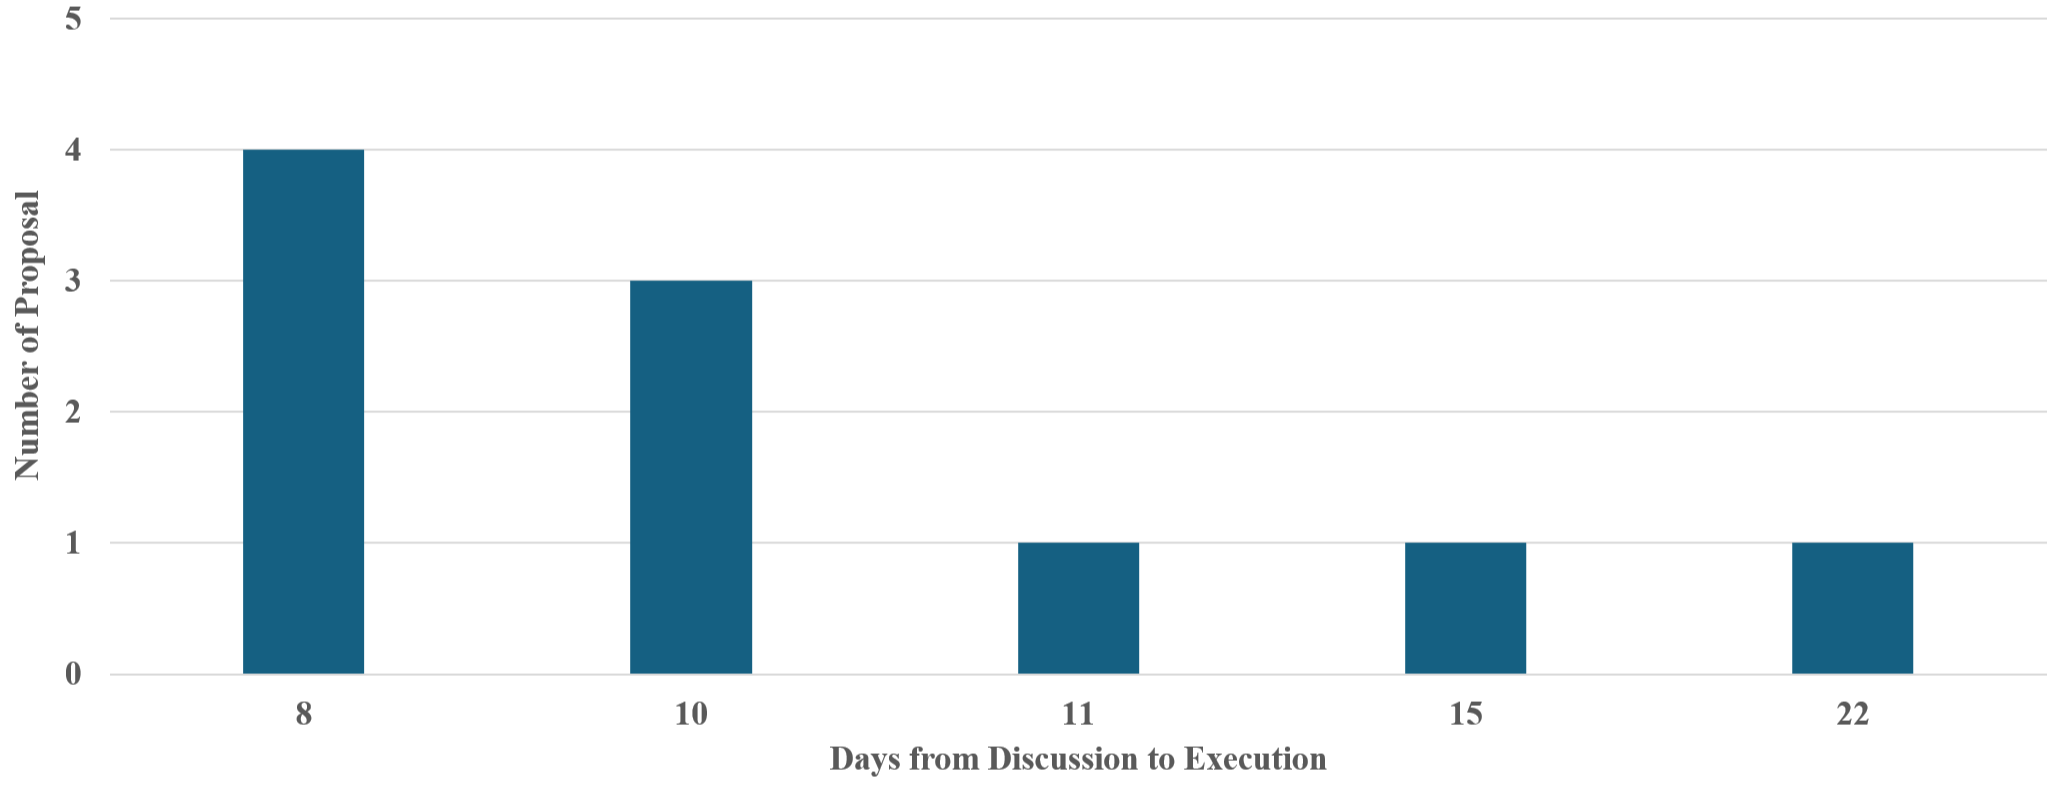
\includegraphics[width=\linewidth]{figure/days_diss_exe.png}}

\end{figure}





\clearpage
\newpage




\begin{landscape}
\begin{figure}[ht!]
\centering
\caption{ Lending Rate}\label{fig:lendingtrate_major}
\caption*{This figure plots the lending rate of lending pools of USDC, DAI, WBTC, and WETH on AAVE and Compound and The Secured Overnight Financing Rate from January 2021 to January 2023.  }

\centering
\subfloat[USD Coin (USDC)]{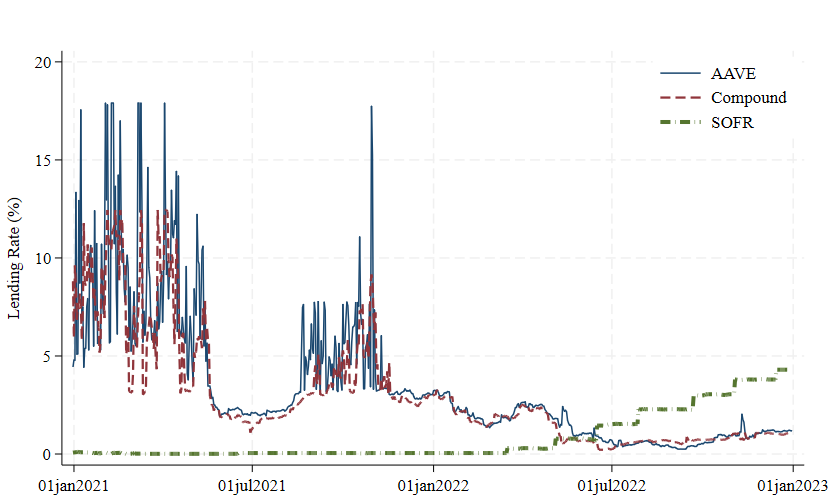
\includegraphics[width=0.45\linewidth]{figure/USDC_LRate.png}}
\subfloat[Dai (DAI)]{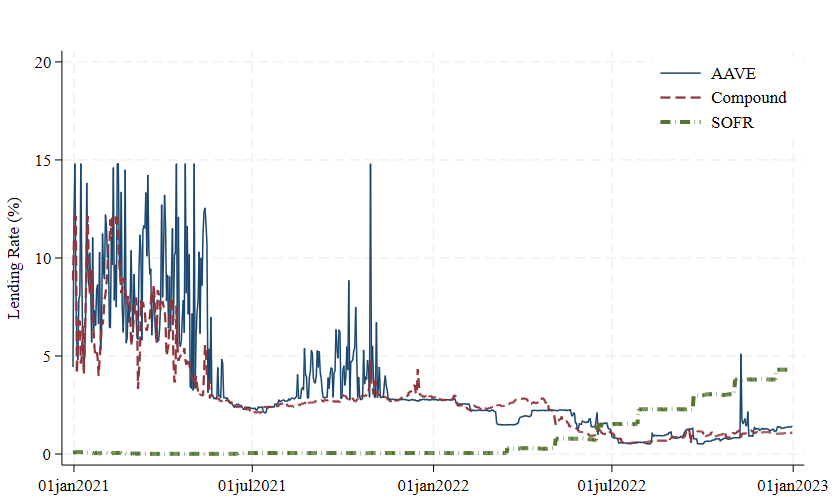
\includegraphics[width=0.45\linewidth]{figure/DAI_LRate.png}}

\subfloat[Wrapped Bitcoin (WBTC)]{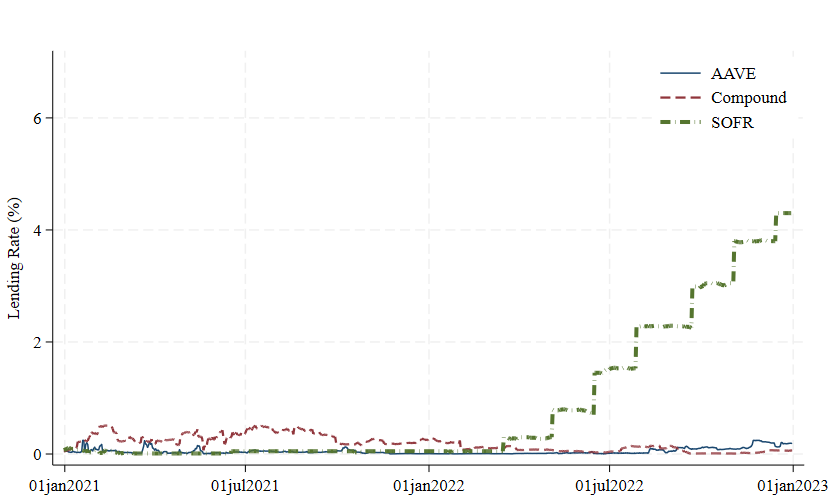
\includegraphics[width=0.45\linewidth]{figure/WBTC_LRate.png}}
\subfloat[Wrapped Ethereum (WETH)]{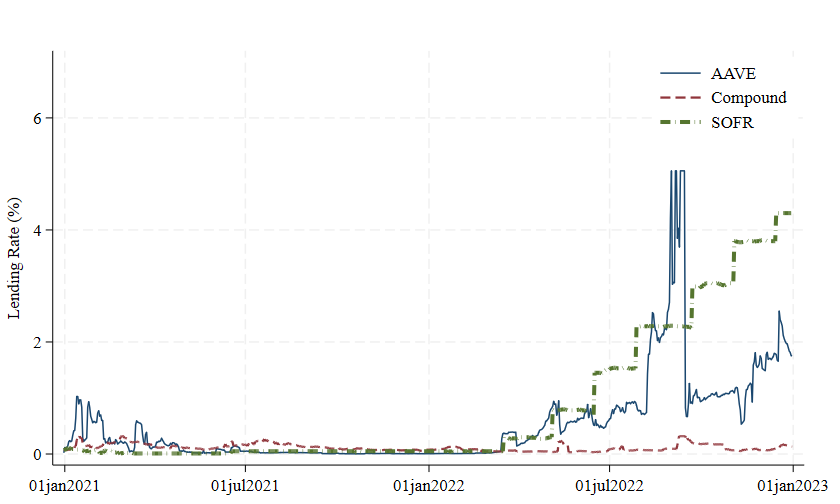
\includegraphics[width=0.45\linewidth]{figure/WETH_LRate.png}}

\end{figure}

\end{landscape}


\clearpage
\newpage
\begin{figure}[ht!]
\centering
\caption{Borrowing and Lending Rate of Other Cryptocurrencies }\label{fig:defi_interestrate_others}
\caption*{This figure plots the lending rate of lending pools other than USDC, DAI, WBTC, and WETH on AAVE and Compound and The Secured Overnight Financing Rate from January 2021 to January 2023. The borrowing (lending) rate is the loan (deposit) amount weighted average of individual cryptocurrencies.}
\subfloat[Borrowing Rate]{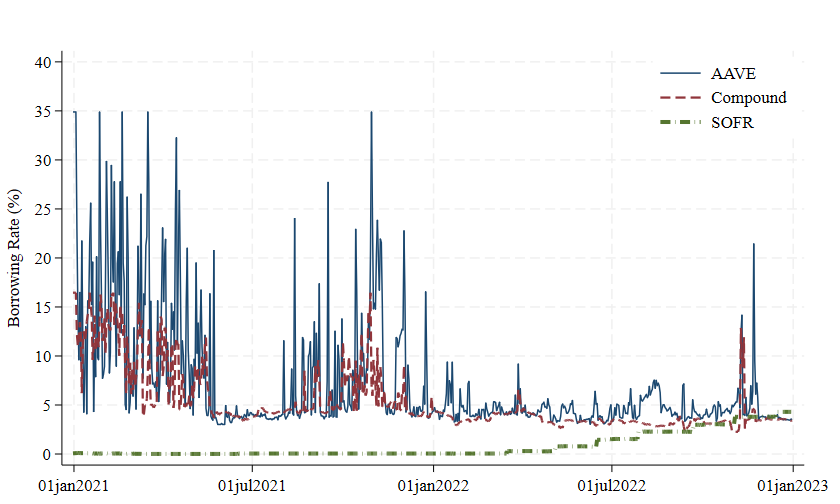
\includegraphics[width=0.9\linewidth]{figure/Others_BRate.png}}


\subfloat[Lending Rate]{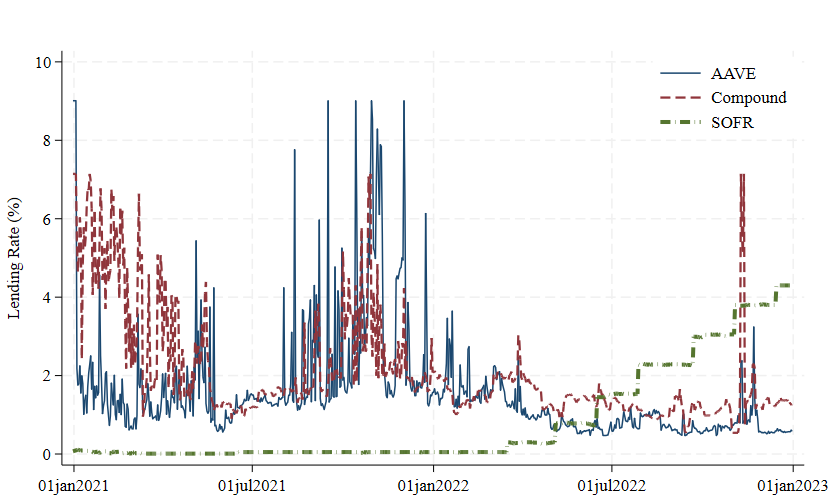
\includegraphics[width=0.9\linewidth]{figure/Others_LRate.png}}

\end{figure}
\clearpage
\newpage


\begin{landscape}
\begin{figure}[ht!]
\centering
\caption{Dynamics of Leverage for Experienced Borrowers}\label{figA:dynamics_lev_experienced}
\caption*{This figure repeats the analysis in Figure \ref{fig:dynamics_lev} using a subsample of experienced borrowers. Experienced borrowers have an account age greater than the median age. Standard errors are clustered at the borrower and week levels. The bars surrounding each coefficient represent the 5\% and 95\% confidence intervals. }

\centering
\subfloat[USD Coin (USDC)]{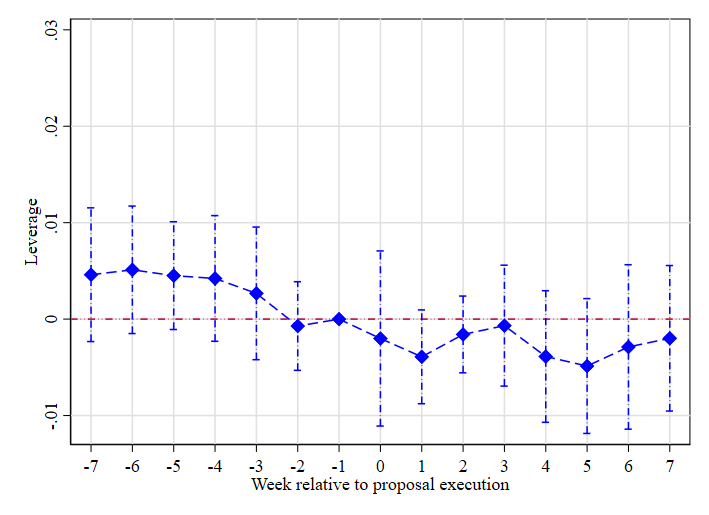
\includegraphics[width=0.4\linewidth]{figure/Heterogeneity/lev_g1_age2.png}}
\subfloat[Dai (DAI)]{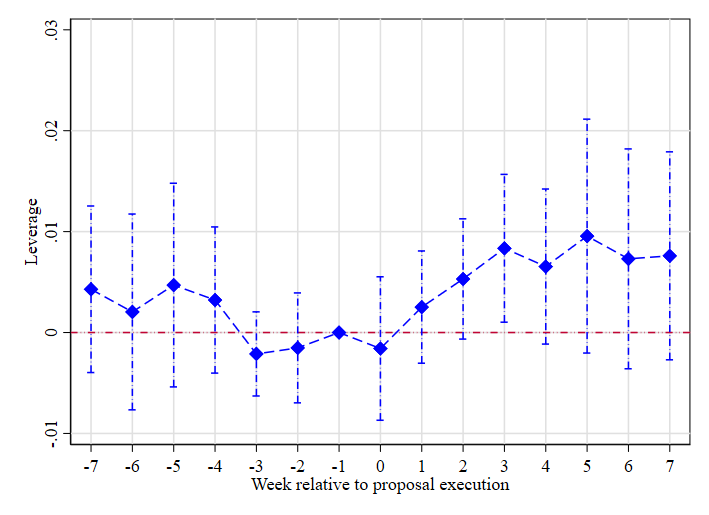
\includegraphics[width=0.4\linewidth]{figure/Heterogeneity/lev_g2_age2.png}}

\subfloat[Wrapped Bitcoin (WBTC)]{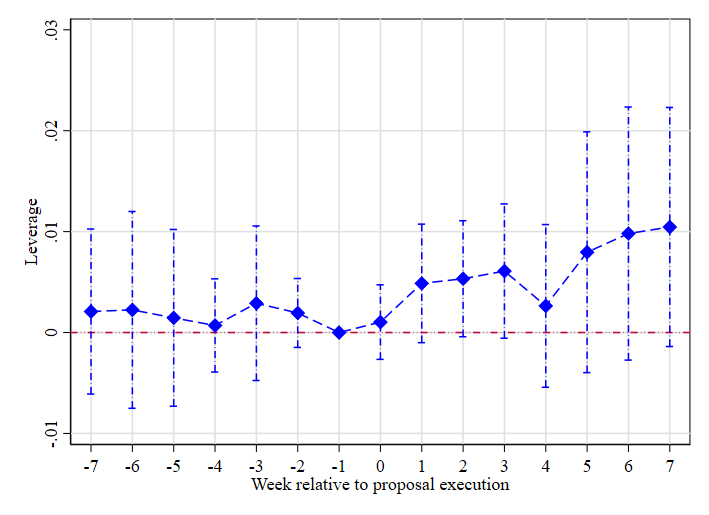
\includegraphics[width=0.4\linewidth]{figure/Heterogeneity/lev_g3_age3.png}}
\subfloat[Wrapped Ethereum (WETH)]{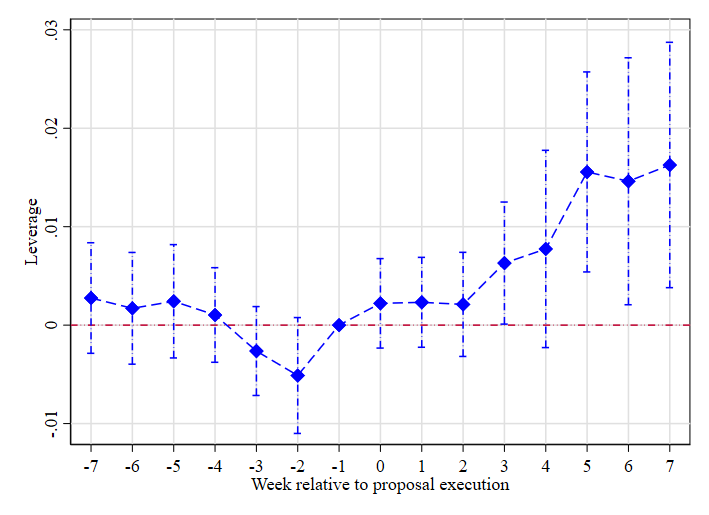
\includegraphics[width=0.4\linewidth]{figure/Heterogeneity/lev_g4_age4.png}}


\end{figure}

\end{landscape}

\clearpage
\newpage

%%%%%%%%%%%% Tables %%%%%%%%%%%%%%%
\clearpage
\newpage
%\setlength{\tabcolsep}{1pt}
    

\begin{table}[ht!]
\small 
\caption{Lending Pools on AAVE and Compound}\label{tabA:lendingpools}
\caption*{This table presents a summary of all lending pools on AAVE (Panel A) and Compound (Panel B). The information includes the names of the lending pools, symbols of lending pools, and whether users can borrow from or use deposits in lending pools as collateral in January 2023.   }

\centering
\def\sym#1{\ifmmode^{#1}\else\(^{#1}\)\fi}

\begin{tabular*}{\linewidth}{@{\extracolsep{\fill}}lllcc}
    \toprule
    Number & Pool Name & Pool Symbol & Can Borrow From? & Can Use as Collateral? \\
    \midrule
    \multicolumn{5}{c}{Panel A: AAVE} \\
    \midrule
    AAVE-1 & TrueUSD & TUSD  & Yes   & Yes \\
    AAVE-2 & Rai Reflex Index & RAI   & \multicolumn{2}{c}{Closed} \\
    AAVE-3 & Gemini dollar & GUSD  & No    & Yes \\
    AAVE-4 & yearn.finance & YFI   & \multicolumn{2}{c}{Closed} \\
    AAVE-5 & Basic Attention Token & BAT   & \multicolumn{2}{c}{Closed} \\
    AAVE-6 & Decentraland MANA & MANA  & \multicolumn{2}{c}{Closed} \\
    AAVE-7 & 1INCH Token & 1INCH & No    & Yes \\
    AAVE-8 & DefiPulse Index & DPI   & No    & Yes \\
    AAVE-9 & Uniswap & UNI   & No    & Yes \\
    AAVE-10 & Wrapped BTC & WBTC  & Yes   & Yes \\
    AAVE-11 & Republic Token & REN   & \multicolumn{2}{c}{Closed} \\
    AAVE-12 & Convex Token & CVX   & \multicolumn{2}{c}{Closed} \\
    AAVE-13 & Binance USD & BUSD  & Yes   & No \\
    AAVE-14 & ChainLink Token & LINK  & No    & Yes \\
    AAVE-15 & Synth sUSD & sUSD  & No    & Yes \\
    AAVE-16 & LUSD Stablecoin & LUSD  & No    & Yes \\
    AAVE-17 & Dai Stablecoin & DAI   & Yes   & Yes \\
    AAVE-18 & Aave Token & AAVE  & No    & Yes \\
    AAVE-19 & Frax  & FRAX  & Yes   & No \\
    AAVE-20 & SushiBar & xSUSHI & \multicolumn{2}{c}{Closed} \\
    AAVE-21 & Paxos Standard & PAX   & No    & Yes \\
    AAVE-22 & Fei USD & FEI   & \multicolumn{2}{c}{Closed} \\
    AAVE-23 & Maker & MKR   & No    & Yes \\
    AAVE-24 & USD Coin & USDC  & Yes   & Yes \\
    AAVE-25 & UST (Wormhole) & UST   & \multicolumn{2}{c}{Closed} \\
    AAVE-26 & Liquid staked Ether 2.0 & stETH & No    & Yes \\
    AAVE-27 & Balancer & BAL   & \multicolumn{2}{c}{Closed} \\
    AAVE-28 & Synthetix Network Token & SNX   & No    & Yes \\
    AAVE-29 & Wrapped Ether & WETH  & Yes   & Yes \\
    AAVE-30 & Ethereum Name Service & ENS   & No    & Yes \\
    AAVE-31 & Ampleforth & AMPL  & \multicolumn{2}{c}{Closed} \\
    AAVE-32 & renFIL & renFIL & \multicolumn{2}{c}{Closed} \\
    AAVE-33 & Curve DAO Token & CRV   & No    & Yes \\
    AAVE-34 & Tether USD & USDT  & Yes   & No \\
    AAVE-35 & Kyber Network Crystal & KNC   & Yes   & Yes \\
    AAVE-36 & 0x Protocol Token & ZRX   & \multicolumn{2}{c}{Closed} \\
    AAVE-37 & Enjin Coin & ENJ   & \multicolumn{2}{c}{Closed} \\
    \bottomrule
        \\ \multicolumn{5}{r}{\textit{(continued on next page)}}\\
          \end{tabular*} 

\end{table}%

\clearpage
\newpage


\begin{table}[ht!]
\small
\centering
\caption*{Table \ref*{tabA:lendingpools} -- Continued from previous page}

\begin{tabular*}{\linewidth}{@{\extracolsep{\fill}}lllcc}
    \toprule
    Number & Pool Name & Pool Symbol & Can Borrow From? & Can Use as Collateral? \\
    \midrule
    \multicolumn{5}{c}{Panel B: Compound} \\
    \midrule
    COMP-1 & Aave Token & AAVE  & Yes   & Yes \\
    COMP-2 & Basic Attention Token & BAT   & Yes   & Yes \\
    COMP-3 & Compound & COMP  & Yes   & Yes \\
    COMP-4 & Dai Stablecoin & DAI   & Yes   & Yes \\
    COMP-5 & Dai Stablecoin v1.0 & DAI   & \multicolumn{2}{c}{Closed} \\
    COMP-6 & Fei USD & FEI   & \multicolumn{2}{c}{Closed} \\
    COMP-7 & ChainLink Token & LINK  & Yes   & Yes \\
    COMP-8 & Maker & MKR   & Yes   & Yes \\
    COMP-9 & Reputation & REP   & \multicolumn{2}{c}{Closed} \\
    COMP-10 & SushiToken & SUSHI & Yes   & Yes \\
    COMP-11 & TrueUSD & TUSD  & Yes   & No \\
    COMP-12 & Uniswap & UNI   & Yes   & Yes \\
    COMP-13 & USD Coin & USDC  & Yes   & Yes \\
    COMP-14 & Pax Dollar & USDP  & Yes   & No \\
    COMP-15 & Tether USD & USDT  & Yes   & No \\
    COMP-16 & Wrapped BTC & WBTC  & Yes   & Yes \\
    COMP-17 & Wrapped Ether & WETH  & Yes   & Yes \\
    COMP-18 & yearn.finance & YFI   & Yes   & Yes \\
    COMP-19 & 0x Protocol Token & ZRX   & Yes   & Yes \\
    \bottomrule
          \end{tabular*} 
 

\end{table}

\clearpage
\newpage
%\setlength{\tabcolsep}{1pt}
    

\begin{table}[ht!]
%\footnotesize 
\caption{Summary Statistics of Borrowing and Lending Positions by Events}\label{tabA:sumstat_bypool}
\caption*{This table presents summary statistics of borrowing and lending positions for each event. Table \ref{tab:proposal_margin} lists the proposal ID and the treated and control pools in each event. $Deposit$ is the US dollar amount (in thousands) of the deposit balance in the treated or control pool. $TotalDeposit$ is the aggregated deposit balance in thousands, calculated by summing the US dollar amounts across all lending positions on the platform. $TotalBorrow$ is the aggregated loan balance in thousands, calculated by summing the dollar amounts across all borrowing positions on the platform. $Leverage$ is the ratio of the total market value of assets ($TotalDeposit+Total Borrow$) and the equity value ($Total Deposit$). Panel A presents the summary statistics of borrowing and lending positions, and Panel B compares the borrowing and lending positions between the treatment and control groups, using observations at the end of the week before the proposal discussion. All financial variables are winsorized at the 1$^{st}$ and 99$^{th}$ percentiles. }

\centering
\def\sym#1{\ifmmode^{#1}\else\(^{#1}\)\fi}






\end{table}%

\clearpage
\newpage
%\setlength{\tabcolsep}{1pt}
    

\begin{table}[ht!]
\footnotesize 
% \caption*{ }

\centering
\def\sym#1{\ifmmode^{#1}\else\(^{#1}\)\fi}


\begin{tabular*}{\linewidth}{@{\extracolsep{\fill}}lcccccc }
    \multicolumn{7}{c}{Appendix Table \ref{tabA:sumstat_bypool} - Proposal AAVE-69 (Treated: AAVE-USDC, Control: COMP-USDC)} \\
    \toprule
     Variable  &N & Mean & SD & P25 & Median & P75 \\
     \midrule
    \multicolumn{7}{c}{Panel A: Summary Statistics on Borrower Account-Week Data} \\
    \midrule
    Deposit (\$, thousand) & 15,740 & 232.65 & 1,059.69 & 0.50  & 3.33  & 45.44 \\
          &       &       &       &       &       &  \\
    TotalDeposit (\$, thousand) & 15,740 & 419.32 & 1,697.89 & 1.59  & 13.74 & 129.59 \\
          &       &       &       &       &       &  \\
    TotalBorrow (\$, thousand) & 15,740 & 149.62 & 607.14 & 0.53  & 5.08  & 49.94 \\
          &       &       &       &       &       &  \\
    Leverage & 15,193 & 1.49  & 0.23  & 1.34  & 1.52  & 1.67 \\
    \midrule
        \multicolumn{7}{c}{Panel B: Differences across the Treated and Control Borrowers} \\
\midrule
          & \multicolumn{2}{c}{Control} &       & \multicolumn{2}{c}{Treated} &  \\
\cmidrule{2-3}\cmidrule{5-6}          & N & Mean &       & N & Mean & Difference \\
\cmidrule{2-3}\cmidrule{5-6}          & (1) & (2) &       & (3) & (4) & (4)-(2) \\
\cmidrule{2-7}    Deposit (\$, thousand) & 318   & 371.28 &       & 734   & 246.44 & -124.84 \\
          &       &       &       &       &       & (78.79) \\
    TotalDeposit (\$, thousand) & 318   & 650.25 &       & 734   & 451.13 & -199.12 \\
          &       &       &       &       &       & (126.68) \\
    TotalBorrow (\$, thousand) & 318   & 212.19 &       & 734   & 180.31 & -31.88 \\
          &       &       &       &       &       & (47.16) \\
    Leverage & 318   & 1.47  &       & 734   & 1.49  & 0.02 \\
          &       &       &       &       &       & (0.02) \\
    \bottomrule
              &       &       &       &       &       &  \\
      \multicolumn{7}{c}{Appendix Table \ref{tabA:sumstat_bypool} - Proposal AAVE-92 (Treated: AAVE-DAI, Control: COMP-DAI)} \\
      \toprule
     Variable  &N & Mean & SD & P25 & Median & P75 \\
     \midrule
    \multicolumn{7}{c}{Panel A: Summary Statistics on Borrower Account-Week Data} \\
    \midrule
    Deposit (\$, thousand) & 8,541 & 71.94 & 540.88 & 0.29  & 1.12  & 9.72 \\
          &       &       &       &       &       &  \\
    TotalDeposit (\$, thousand) & 8,541 & 157.70 & 940.19 & 0.62  & 3.56  & 33.53 \\
          &       &       &       &       &       &  \\
    TotalBorrow (\$, thousand) & 8,541 & 61.37 & 358.37 & 0.25  & 1.44  & 11.44 \\
          &       &       &       &       &       &  \\
    Leverage & 8,257 & 1.49  & 0.21  & 1.36  & 1.53  & 1.66 \\
    \midrule
        \multicolumn{7}{c}{Panel B: Differences across the Treated and Control Borrowers} \\
\midrule
          & \multicolumn{2}{c}{Control} &       & \multicolumn{2}{c}{Treated} &  \\
\cmidrule{2-3}\cmidrule{5-6}          & N & Mean &       & N & Mean & Difference \\
\cmidrule{2-3}\cmidrule{5-6}          & (1) & (2) &       & (3) & (4) & (4)-(2) \\
\cmidrule{2-7}    Deposit (\$, thousand) & 247   & 70.61 &       & 330   & 108.18 & 37.57 \\
          &       &       &       &       &       & (50.61) \\
    TotalDeposit (\$, thousand) & 247   & 105.88 &       & 330   & 264.95 & 159.07* \\
          &       &       &       &       &       & (93.61) \\
    TotalBorrow (\$, thousand) & 247   & 42.36 &       & 330   & 99.26 & 56.90 \\
          &       &       &       &       &       & (37.42) \\
    Leverage & 247   & 1.50  &       & 330   & 1.47  & -0.03* \\
          &       &       &       &       &       & (0.02) \\
    \bottomrule
          \end{tabular*} 



 \end{table}%

% \clearpage
% \newpage
%\setlength{\tabcolsep}{1pt}
    

% \begin{table}[ht!]
% \footnotesize 
% \caption*{Appendix Table \ref{tabA:sumstat_bypool} - Proposal AAVE-92 (Treated: AAVE-DAI, Control: COMP-DAI)}

% \centering
% \def\sym#1{\ifmmode^{#1}\else\(^{#1}\)\fi}


% \begin{tabular*}{\linewidth}{@{\extracolsep{\fill}}lcccccc }
%     \toprule
%      Variable  &N & Mean & SD & P25 & Median & P75 \\
%      \midrule
%     \multicolumn{7}{c}{Panel A: Summary Statistics on Borrower Account-Week Data} \\
%     \midrule
%     Deposit (\$, thousand) & 8,541 & 71.94 & 540.88 & 0.29  & 1.12  & 9.72 \\
%           &       &       &       &       &       &  \\
%     TotalDeposit (\$, thousand) & 8,541 & 157.70 & 940.19 & 0.62  & 3.56  & 33.53 \\
%           &       &       &       &       &       &  \\
%     TotalBorrow (\$, thousand) & 8,541 & 61.37 & 358.37 & 0.25  & 1.44  & 11.44 \\
%           &       &       &       &       &       &  \\
%     Leverage & 8,257 & 1.49  & 0.21  & 1.36  & 1.53  & 1.66 \\
%     \midrule
%         \multicolumn{7}{c}{Panel B: Differences across the Treated and Control Borrowers} \\
% \midrule
%           & \multicolumn{2}{c}{Control} &       & \multicolumn{2}{c}{Treated} &  \\
% \cmidrule{2-3}\cmidrule{5-6}          & N & Mean &       & N & Mean & Difference \\
% \cmidrule{2-3}\cmidrule{5-6}          & (1) & (2) &       & (3) & (4) & (4)-(2) \\
% \cmidrule{2-7}    Deposit (\$, thousand) & 247   & 70.61 &       & 330   & 108.18 & 37.57 \\
%           &       &       &       &       &       & (50.61) \\
%     TotalDeposit (\$, thousand) & 247   & 105.88 &       & 330   & 264.95 & 159.07* \\
%           &       &       &       &       &       & (93.61) \\
%     TotalBorrow (\$, thousand) & 247   & 42.36 &       & 330   & 99.26 & 56.90 \\
%           &       &       &       &       &       & (37.42) \\
%     Leverage & 247   & 1.50  &       & 330   & 1.47  & -0.03* \\
%           &       &       &       &       &       & (0.02) \\
%     \bottomrule
%           \end{tabular*} 



% \end{table}%

\clearpage
\newpage
%\setlength{\tabcolsep}{1pt}
    

\begin{table}[ht!]
\footnotesize 
% \caption*{Appendix Table \ref{tabA:sumstat_bypool} - Proposal AAVE-94 (Treated: AAVE-WBTC, Control: COMP-WBTC)}

\centering
\def\sym#1{\ifmmode^{#1}\else\(^{#1}\)\fi}


\begin{tabular*}{\linewidth}{@{\extracolsep{\fill}}lcccccc }
      \multicolumn{7}{c}{Appendix Table \ref{tabA:sumstat_bypool} - Proposal AAVE-94 (Treated: AAVE-WBTC, Control: COMP-WBTC)} \\
    \toprule
     Variable  &N & Mean & SD & P25 & Median & P75 \\
     \midrule
    \multicolumn{7}{c}{Panel A: Summary Statistics on Borrower Account-Week Data} \\
    \midrule
    Deposit (\$, thousand) & 24,825 & 290.66 & 1,137.83 & 2.38  & 19.17 & 85.81 \\
          &       &       &       &       &       &  \\
    TotalDeposit (\$, thousand) & 24,825 & 523.01 & 1,879.95 & 7.24  & 39.94 & 190.05 \\
          &       &       &       &       &       &  \\
    TotalBorrow (\$, thousand) & 24,825 & 194.81 & 696.48 & 2.86  & 14.56 & 70.08 \\
          &       &       &       &       &       &  \\
    Leverage & 24,086 & 1.43  & 0.17  & 1.32  & 1.44  & 1.55 \\
    \midrule
        \multicolumn{7}{c}{Panel B: Differences across the Treated and Control Borrowers} \\
\midrule
          & \multicolumn{2}{c}{Control} &       & \multicolumn{2}{c}{Treated} &  \\
\cmidrule{2-3}\cmidrule{5-6}          & N & Mean &       & N & Mean & Difference \\
\cmidrule{2-3}\cmidrule{5-6}          & (1) & (2) &       & (3) & (4) & (4)-(2) \\
\cmidrule{2-7}    Deposit (\$, thousand) & 531   & 418.46 &       & 1,124 & 334.95 & -83.51 \\
          &       &       &       &       &       & (68.41) \\
    TotalDeposit (\$, thousand) & 531   & 778.19 &       & 1,124 & 573.76 & -204.43* \\
          &       &       &       &       &       & (111.89) \\
    TotalBorrow (\$, thousand) & 531   & 257.95 &       & 1,124 & 201.75 & -56.20 \\
          &       &       &       &       &       & (39.62) \\
    Leverage & 531   & 1.37  &       & 1,124 & 1.38  & 0.01** \\
          &       &       &       &       &       & (0.00) \\
    \bottomrule
          &       &       &       &       &       &  \\
      \multicolumn{7}{c}{Appendix Table \ref{tabA:sumstat_bypool} - Proposal AAVE-102 (Treated: AAVE-USDC, Control: COMP-USDC)} \\
  \toprule
     Variable  &N & Mean & SD & P25 & Median & P75 \\
     \midrule
    \multicolumn{7}{c}{Panel A: Summary Statistics on Borrower Account-Week Data} \\
    \midrule
    Deposit (\$, thousand) & 19,968 & 258.89 & 1,105.99 & 0.54  & 5.84  & 53.90 \\
          &       &       &       &       &       &  \\
    TotalDeposit (\$, thousand) & 19,968 & 393.31 & 1,633.30 & 1.51  & 16.03 & 116.95 \\
          &       &       &       &       &       &  \\
    TotalBorrow (\$, thousand) & 19,968 & 163.76 & 662.06 & 0.54  & 6.09  & 50.03 \\
          &       &       &       &       &       &  \\
    Leverage & 19,138 & 1.52  & 0.24  & 1.36  & 1.55  & 1.71 \\
    \midrule
        \multicolumn{7}{c}{Panel B: Differences across the Treated and Control Borrowers} \\
\midrule
          & \multicolumn{2}{c}{Control} &       & \multicolumn{2}{c}{Treated} &  \\
\cmidrule{2-3}\cmidrule{5-6}          & N & Mean &       & N & Mean & Difference \\
\cmidrule{2-3}\cmidrule{5-6}          & (1) & (2) &       & (3) & (4) & (4)-(2) \\
\cmidrule{2-7}    Deposit (\$, thousand) & 295   & 341.63 &       & 1,025 & 319.37 & -22.26 \\
          &       &       &       &       &       & (84.07) \\
    TotalDeposit (\$, thousand) & 295   & 471.89 &       & 1,025 & 453.24 & -18.65 \\
          &       &       &       &       &       & (119.96) \\
    TotalBorrow (\$, thousand) & 295   & 144.00 &       & 1,025 & 185.34 & 41.34 \\
          &       &       &       &       &       & (45.21) \\
    Leverage & 295   & 1.46  &       & 1,025 & 1.53  & 0.07*** \\
          &       &       &       &       &       & (0.02) \\
    \bottomrule
    
          \end{tabular*} 



\end{table}%


% \clearpage
% \newpage
% \begin{table}[ht!]
% %\footnotesize 
% \caption*{Appendix Table \ref{tabA:sumstat_bypool} - Proposal AAVE-102 (Treated: AAVE-USDC, Control: COMP-USDC)}

% \centering
% \def\sym#1{\ifmmode^{#1}\else\(^{#1}\)\fi}


% \begin{tabular*}{\linewidth}{@{\extracolsep{\fill}}lcccccc }
%     \toprule
%      Variable  &N & Mean & SD & P25 & Median & P75 \\
%      \midrule
%     \multicolumn{7}{c}{Panel A: Summary Statistics on Borrower Account-Week Data} \\
%     \midrule
%     Deposit (\$, thousand) & 19,968 & 258.89 & 1105.99 & 0.54  & 5.84  & 53.90 \\
%           &       &       &       &       &       &  \\
%     TotalDeposit (\$, thousand) & 19,968 & 393.31 & 1633.30 & 1.51  & 16.03 & 116.95 \\
%           &       &       &       &       &       &  \\
%     TotalBorrow (\$, thousand) & 19,968 & 163.76 & 662.06 & 0.54  & 6.09  & 50.03 \\
%           &       &       &       &       &       &  \\
%     Leverage & 19,138 & 1.52  & 0.24  & 1.36  & 1.55  & 1.71 \\
%     \midrule
%         \multicolumn{7}{c}{Panel B: Differences across the Treated and Control Borrowers} \\
% \midrule
%           & \multicolumn{2}{c}{Control} &       & \multicolumn{2}{c}{Treated} &  \\
% \cmidrule{2-3}\cmidrule{5-6}          & N & Mean &       & N & Mean & Difference \\
% \cmidrule{2-3}\cmidrule{5-6}          & (1) & (2) &       & (3) & (4) & (4)-(2) \\
% \cmidrule{2-7}    Deposit (\$, thousand) & 295   & 341.63 &       & 1,025 & 319.37 & -22.26 \\
%           &       &       &       &       &       & (84.07) \\
%     TotalDeposit (\$, thousand) & 295   & 471.89 &       & 1,025 & 453.24 & -18.65 \\
%           &       &       &       &       &       & (119.96) \\
%     TotalBorrow (\$, thousand) & 295   & 144.00 &       & 1,025 & 185.34 & 41.34 \\
%           &       &       &       &       &       & (45.21) \\
%     Leverage & 295   & 1.46  &       & 1,025 & 1.53  & 0.07*** \\
%           &       &       &       &       &       & (0.02) \\
%     \bottomrule
%           \end{tabular*} 



% \end{table}%

\clearpage
\newpage
\begin{table}[ht!]
\footnotesize 
% \caption*{Appendix Table \ref{tabA:sumstat_bypool} - Proposal AAVE-102 (Treated: AAVE-WETH, Control: COMP-WETH)}

\centering
\def\sym#1{\ifmmode^{#1}\else\(^{#1}\)\fi}


\begin{tabular*}{\linewidth}{@{\extracolsep{\fill}}lcccccc }
      \multicolumn{7}{c}{Appendix Table \ref{tabA:sumstat_bypool} - Proposal AAVE-102 (Treated: AAVE-WETH, Control: COMP-WETH)} \\
    \toprule
     Variable  &N & Mean & SD & P25 & Median & P75 \\
     \midrule
    \multicolumn{7}{c}{Panel A: Summary Statistics on Borrower Account-Week Data} \\
    \midrule
    Deposit (\$, thousand) & 66,360 & 152.10 & 787.66 & 0.78  & 5.37  & 35.12 \\
          &       &       &       &       &       &  \\
    TotalDeposit (\$, thousand) & 66,360 & 251.52 & 1,247.01 & 1.35  & 9.83  & 61.36 \\
          &       &       &       &       &       &  \\
    TotalBorrow (\$, thousand) & 66,360 & 95.79 & 474.79 & 0.52  & 3.71  & 24.46 \\
          &       &       &       &       &       &  \\
    Leverage & 64,861 & 1.46  & 0.20  & 1.33  & 1.47  & 1.60 \\
    \midrule
        \multicolumn{7}{c}{Panel B: Differences across the Treated and Control Borrowers} \\
\midrule
          & \multicolumn{2}{c}{Control} &       & \multicolumn{2}{c}{Treated} &  \\
\cmidrule{2-3}\cmidrule{5-6}          & N & Mean &       & N & Mean & Difference \\
\cmidrule{2-3}\cmidrule{5-6}          & (1) & (2) &       & (3) & (4) & (4)-(2) \\
\cmidrule{2-7}    Deposit (\$, thousand) & 1,263 & 181.64 &       & 3,137 & 149.43 & -32.21 \\
          &       &       &       &       &       & (26.58) \\
    TotalDeposit (\$, thousand) & 1,263 & 282.63 &       & 3,137 & 249.67 & -32.96 \\
          &       &       &       &       &       & (42.08) \\
    TotalBorrow (\$, thousand) & 1,263 & 107.20 &       & 3,137 & 99.55 & -7.65 \\
          &       &       &       &       &       & (16.54) \\
    Leverage & 1,263 & 1.46  &       & 3,137 & 1.46  & 0.00 \\
          &       &       &       &       &       & (0.01) \\
    \bottomrule

              &       &       &       &       &       &  \\
      \multicolumn{7}{c}{Appendix Table \ref{tabA:sumstat_bypool} - Proposal AAVE-108 (Treated: AAVE-WBTC, Control: COMP-WBTC)} \\
         \toprule
     Variable  &N & Mean & SD & P25 & Median & P75 \\
     \midrule
    \multicolumn{7}{c}{Panel A: Summary Statistics on Borrower Account-Week Data} \\
    \midrule
    Deposit (\$, thousand) & 25,944 & 270.15 & 1,096.22 & 1.98  & 16.36 & 76.11 \\
          &       &       &       &       &       &  \\
    TotalDeposit (\$, thousand) & 25,944 & 476.90 & 1,760.83 & 6.60  & 37.01 & 167.35 \\
          &       &       &       &       &       &  \\
    TotalBorrow (\$, thousand) & 25,944 & 189.29 & 685.59 & 2.50  & 13.54 & 65.44 \\
          &       &       &       &       &       &  \\
    Leverage & 25,169 & 1.45  & 0.18  & 1.33  & 1.47  & 1.58 \\
    \midrule
        \multicolumn{7}{c}{Panel B: Differences across the Treated and Control Borrowers} \\
\midrule
          & \multicolumn{2}{c}{Control} &       & \multicolumn{2}{c}{Treated} &  \\
\cmidrule{2-3}\cmidrule{5-6}          & N & Mean &       & N & Mean & Difference \\
\cmidrule{2-3}\cmidrule{5-6}          & (1) & (2) &       & (3) & (4) & (4)-(2) \\
\cmidrule{2-7}    Deposit (\$, thousand) & 509   & 348.42 &       & 1,220 & 270.17 & -78.25 \\
          &       &       &       &       &       & (59.50) \\
    TotalDeposit (\$, thousand) & 509   & 588.22 &       & 1,220 & 452.52 & -135.70 \\
          &       &       &       &       &       & (93.89) \\
    TotalBorrow (\$, thousand) & 509   & 227.95 &       & 1,220 & 178.60 & -49.35 \\
          &       &       &       &       &       & (35.86) \\
    Leverage & 509   & 1.46  &       & 1,220 & 1.45  & 0.01 \\
          &       &       &       &       &       & (0.01) \\
    \bottomrule
          \end{tabular*} 



\end{table}%

% \clearpage
% \newpage
% \begin{table}[ht!]
% %\footnotesize 
% \caption*{Appendix Table \ref{tabA:sumstat_bypool} - Proposal AAVE-108 (Treated: AAVE-WBTC, Control: COMP-WBTC)}

% \centering
% \def\sym#1{\ifmmode^{#1}\else\(^{#1}\)\fi}


% \begin{tabular*}{\linewidth}{@{\extracolsep{\fill}}lcccccc }
%     \toprule
%      Variable  &N & Mean & SD & P25 & Median & P75 \\
%      \midrule
%     \multicolumn{7}{c}{Panel A: Summary Statistics on Borrower Account-Week Data} \\
%     \midrule
%     Deposit (\$, thousand) & 25,944 & 270.15 & 1096.22 & 1.98  & 16.36 & 76.11 \\
%           &       &       &       &       &       &  \\
%     TotalDeposit (\$, thousand) & 25,944 & 476.90 & 1760.83 & 6.60  & 37.01 & 167.35 \\
%           &       &       &       &       &       &  \\
%     TotalBorrow (\$, thousand) & 25,944 & 189.29 & 685.59 & 2.50  & 13.54 & 65.44 \\
%           &       &       &       &       &       &  \\
%     Leverage & 25,169 & 1.45  & 0.18  & 1.33  & 1.47  & 1.58 \\
%     \midrule
%         \multicolumn{7}{c}{Panel B: Differences across the Treated and Control Borrowers} \\
% \midrule
%           & \multicolumn{2}{c}{Control} &       & \multicolumn{2}{c}{Treated} &  \\
% \cmidrule{2-3}\cmidrule{5-6}          & N & Mean &       & N & Mean & Difference \\
% \cmidrule{2-3}\cmidrule{5-6}          & (1) & (2) &       & (3) & (4) & (4)-(2) \\
% \cmidrule{2-7}    Deposit (\$, thousand) & 509   & 348.42 &       & 1,220 & 270.17 & -78.25 \\
%           &       &       &       &       &       & (59.50) \\
%     TotalDeposit (\$, thousand) & 509   & 588.22 &       & 1,220 & 452.52 & -135.70 \\
%           &       &       &       &       &       & (93.89) \\
%     TotalBorrow (\$, thousand) & 509   & 227.95 &       & 1,220 & 178.60 & -49.35 \\
%           &       &       &       &       &       & (35.86) \\
%     Leverage & 509   & 1.46  &       & 1,220 & 1.45  & 0.01 \\
%           &       &       &       &       &       & (0.01) \\
%     \bottomrule
%           \end{tabular*} 



% \end{table}%

\clearpage
\newpage
\begin{table}[ht!]
\footnotesize 
% \caption*{Appendix Table \ref{tabA:sumstat_bypool} - Proposal COMP-36 (Treated: COMP-WBTC, Control: AAVE-WBTC)}

\centering
\def\sym#1{\ifmmode^{#1}\else\(^{#1}\)\fi}


\begin{tabular*}{\linewidth}{@{\extracolsep{\fill}}lcccccc }
      \multicolumn{7}{c}{Appendix Table \ref{tabA:sumstat_bypool} - Proposal COMP-36 (Treated: COMP-WBTC, Control: AAVE-WBTC)} \\
      
    \toprule
     Variable  &N & Mean & SD & P25 & Median & P75 \\
     \midrule
    \multicolumn{7}{c}{Panel A: Summary Statistics on Borrower Account-Week Data} \\
    \midrule
    Deposit (\$, thousand) & 16,110 & 382.43 & 1,341.46 & 0.05  & 14.61 & 111.60 \\
          &       &       &       &       &       &  \\
    TotalDeposit (\$, thousand) & 16,110 & 771.81 & 2,361.48 & 5.71  & 56.91 & 320.04 \\
          &       &       &       &       &       &  \\
    TotalBorrow (\$, thousand) & 16,110 & 279.76 & 896.60 & 0.99  & 15.01 & 100.49 \\
          &       &       &       &       &       &  \\
    Leverage & 14,087 & 1.33  & 0.17  & 1.22  & 1.34  & 1.45 \\
    \midrule
        \multicolumn{7}{c}{Panel B: Differences across the Treated and Control Borrowers} \\
\midrule
          & \multicolumn{2}{c}{Control} &       & \multicolumn{2}{c}{Treated} &  \\
\cmidrule{2-3}\cmidrule{5-6}          & N & Mean &       & N & Mean & Difference \\
\cmidrule{2-3}\cmidrule{5-6}          & (1) & (2) &       & (3) & (4) & (4)-(2) \\
\cmidrule{2-7}    Deposit (\$, thousand) & 405   & 239.41 &       & 740   & 632.84 & 393.43*** \\
          &       &       &       &       &       & (88.97) \\
    TotalDeposit (\$, thousand) & 405   & 396.17 &       & 740   & 1,046.41 & 650.24*** \\
          &       &       &       &       &       & (142.83) \\
    TotalBorrow (\$, thousand) & 405   & 149.40 &       & 740   & 341.67 & 192.27*** \\
          &       &       &       &       &       & (52.20) \\
    Leverage & 405   & 1.35  &       & 740   & 1.29  & -0.06*** \\
          &       &       &       &       &       & (0.01) \\
    \bottomrule
              &       &       &       &       &       &  \\
      \multicolumn{7}{c}{Appendix Table \ref{tabA:sumstat_bypool} - Proposal COMP-66 (Treated: COMP-USDC, Control: AAVE-USDC)} \\
       \toprule
     Variable  &N & Mean & SD & P25 & Median & P75 \\
     \midrule
    \multicolumn{7}{c}{Panel A: Summary Statistics on Borrower Account-Week Data} \\
    \midrule
    Deposit (\$, thousand) & 16,383 & 318.85 & 1,322.64 & 0.49  & 3.48  & 40.51 \\
          &       &       &       &       &       &  \\
    TotalDeposit (\$, thousand) & 16,383 & 659.06 & 2,295.55 & 2.25  & 19.97 & 187.18 \\
          &       &       &       &       &       &  \\
    TotalBorrow (\$, thousand) & 16,383 & 254.75 & 901.97 & 0.71  & 6.03  & 60.89 \\
          &       &       &       &       &       &  \\
    Leverage & 15,662 & 1.44  & 0.22  & 1.28  & 1.45  & 1.60 \\
    \midrule
        \multicolumn{7}{c}{Panel B: Differences across the Treated and Control Borrowers} \\
\midrule
          & \multicolumn{2}{c}{Control} &       & \multicolumn{2}{c}{Treated} &  \\
\cmidrule{2-3}\cmidrule{5-6}          & N & Mean &       & N & Mean & Difference \\
\cmidrule{2-3}\cmidrule{5-6}          & (1) & (2) &       & (3) & (4) & (4)-(2) \\
\cmidrule{2-7}    Deposit (\$, thousand) & 688   & 312.82 &       & 414   & 473.14 & 160.32* \\
          &       &       &       &       &       & (87.85) \\
    TotalDeposit (\$, thousand) & 688   & 681.00 &       & 414   & 818.07 & 137.07 \\
          &       &       &       &       &       & (148.10) \\
    TotalBorrow (\$, thousand) & 688   & 255.27 &       & 414   & 322.10 & 66.83 \\
          &       &       &       &       &       & (57.07) \\
    Leverage & 688   & 1.45  &       & 414   & 1.44  & 0.01 \\
          &       &       &       &       &       & (0.01) \\
    \bottomrule
          \end{tabular*} 



\end{table}%

% \clearpage
% \newpage
% \begin{table}[ht!]
% %\footnotesize 
% \caption*{Appendix Table \ref{tabA:sumstat_bypool} - Proposal COMP-66 (Treated: COMP-USDC, Control: AAVE-USDC)}

% \centering
% \def\sym#1{\ifmmode^{#1}\else\(^{#1}\)\fi}


% \begin{tabular*}{\linewidth}{@{\extracolsep{\fill}}lcccccc }
%     \toprule
%      Variable  &N & Mean & SD & P25 & Median & P75 \\
%      \midrule
%     \multicolumn{7}{c}{Panel A: Summary Statistics on Borrower Account-Week Data} \\
%     \midrule
%     Deposit (\$, thousand) & 16,383 & 318.85 & 1322.64 & 0.49  & 3.48  & 40.51 \\
%           &       &       &       &       &       &  \\
%     TotalDeposit (\$, thousand) & 16,383 & 659.06 & 2295.55 & 2.25  & 19.97 & 187.18 \\
%           &       &       &       &       &       &  \\
%     TotalBorrow (\$, thousand) & 16,383 & 254.75 & 901.97 & 0.71  & 6.03  & 60.89 \\
%           &       &       &       &       &       &  \\
%     Leverage & 15,662 & 1.44  & 0.22  & 1.28  & 1.45  & 1.60 \\
%     \midrule
%         \multicolumn{7}{c}{Panel B: Differences across the Treated and Control Borrowers} \\
% \midrule
%           & \multicolumn{2}{c}{Control} &       & \multicolumn{2}{c}{Treated} &  \\
% \cmidrule{2-3}\cmidrule{5-6}          & N & Mean &       & N & Mean & Difference \\
% \cmidrule{2-3}\cmidrule{5-6}          & (1) & (2) &       & (3) & (4) & (4)-(2) \\
% \cmidrule{2-7}    Deposit (\$, thousand) & 688   & 312.82 &       & 414   & 473.14 & 160.32* \\
%           &       &       &       &       &       & (87.85) \\
%     TotalDeposit (\$, thousand) & 688   & 681.00 &       & 414   & 818.07 & 137.07 \\
%           &       &       &       &       &       & (148.10) \\
%     TotalBorrow (\$, thousand) & 688   & 255.27 &       & 414   & 322.10 & 66.83 \\
%           &       &       &       &       &       & (57.07) \\
%     Leverage & 688   & 1.45  &       & 414   & 1.44  & 0.01 \\
%           &       &       &       &       &       & (0.01) \\
%     \bottomrule
%           \end{tabular*} 



% \end{table}%

\clearpage
\newpage
\begin{table}[ht!]
\footnotesize 
% \caption*{Appendix Table \ref{tabA:sumstat_bypool} - Proposal COMP-71 (Treated: COMP-DAI, Control: AAVE-DAI)}

\centering
\def\sym#1{\ifmmode^{#1}\else\(^{#1}\)\fi}


\begin{tabular*}{\linewidth}{@{\extracolsep{\fill}}lcccccc }

      \multicolumn{7}{c}{Appendix Table \ref{tabA:sumstat_bypool} - Proposal COMP-71 (Treated: COMP-DAI, Control: AAVE-DAI)} \\
    \toprule
     Variable  &N & Mean & SD & P25 & Median & P75 \\
     \midrule
    \multicolumn{7}{c}{Panel A: Summary Statistics on Borrower Account-Week Data} \\
    \midrule
    Deposit (\$, thousand) & 10,409 & 98.45 & 659.82 & 0.38  & 1.53  & 13.63 \\
          &       &       &       &       &       &  \\
    TotalDeposit (\$, thousand) & 10,409 & 250.53 & 1,243.26 & 1.22  & 8.64  & 74.73 \\
          &       &       &       &       &       &  \\
    TotalBorrow (\$, thousand) & 10,409 & 101.94 & 531.84 & 0.37  & 2.70  & 23.63 \\
          &       &       &       &       &       &  \\
    Leverage & 10,128 & 1.43  & 0.22  & 1.28  & 1.46  & 1.60 \\
    \midrule
        \multicolumn{7}{c}{Panel B: Differences across the Treated and Control Borrowers} \\
\midrule
          & \multicolumn{2}{c}{Control} &       & \multicolumn{2}{c}{Treated} &  \\
\cmidrule{2-3}\cmidrule{5-6}          & N & Mean &       & N & Mean & Difference \\
\cmidrule{2-3}\cmidrule{5-6}          & (1) & (2) &       & (3) & (4) & (4)-(2) \\
\cmidrule{2-7}    Deposit (\$, thousand) & 347   & 113.54 &       & 346   & 108.64 & -4.90 \\
          &       &       &       &       &       & (54.75) \\
    TotalDeposit (\$, thousand) & 347   & 329.41 &       & 346   & 244.84 & -84.57 \\
          &       &       &       &       &       & (99.93) \\
    TotalBorrow (\$, thousand) & 347   & 136.01 &       & 346   & 93.98 & -42.03 \\
          &       &       &       &       &       & (42.75) \\
    Leverage & 347   & 1.42  &       & 346   & 1.43  & 0.01 \\
          &       &       &       &       &       & (0.02) \\
    \bottomrule
              &       &       &       &       &       &  \\
      \multicolumn{7}{c}{Appendix Table \ref{tabA:sumstat_bypool} - Proposal COMP-71 (Treated: COMP-WETH, Control: AAVE-WETH)} \\
        \toprule
     Variable  &N & Mean & SD & P25 & Median & P75 \\
     \midrule
    \multicolumn{7}{c}{Panel A: Summary Statistics on Borrower Account-Week Data} \\
    \midrule
    Deposit (\$, thousand) & 96,292 & 353.17 & 1,242.78 & 3.92  & 24.32 & 133.69 \\
          &       &       &       &       &       &  \\
    TotalDeposit (\$, thousand) & 96,292 & 532.32 & 1,926.97 & 5.74  & 36.92 & 198.46 \\
          &       &       &       &       &       &  \\
    TotalBorrow (\$, thousand) & 96,292 & 191.22 & 708.57 & 1.50  & 11.00 & 63.22 \\
          &       &       &       &       &       &  \\
              Leverage & 92,413 & 1.37  & 0.19  & 1.24  & 1.36  & 1.51 \\

    \midrule
        \multicolumn{7}{c}{Panel B: Differences across the Treated and Control Borrowers} \\
\midrule
          & \multicolumn{2}{c}{Control} &       & \multicolumn{2}{c}{Treated} &  \\
\cmidrule{2-3}\cmidrule{5-6}          & N & Mean &       & N & Mean & Difference \\
\cmidrule{2-3}\cmidrule{5-6}          & (1) & (2) &       & (3) & (4) & (4)-(2) \\
\cmidrule{2-7}    Deposit (\$, thousand) & 4,184 & 397.45 &       & 2,266 & 507.04 & 109.59*** \\
          &       &       &       &       &       & (35.99) \\
    TotalDeposit (\$, thousand) & 4,184 & 583.10 &       & 2,266 & 773.84 & 190.74*** \\
          &       &       &       &       &       & (55.44) \\
    TotalBorrow (\$, thousand) & 4,184 & 209.79 &       & 2,266 & 235.59 & 25.80 \\
          &       &       &       &       &       & (20.01) \\
    Leverage & 4,184 & 1.35  &       & 2,266 & 1.3   & -0.05*** \\
          &       &       &       &       &       & (0.01) \\
    \bottomrule
          \end{tabular*} 



\end{table}%

% \clearpage
% \newpage
% \begin{table}[ht!]
% %\footnotesize 
% \caption*{Appendix Table \ref{tabA:sumstat_bypool} - Proposal COMP-71 (Treated: COMP-WETH, Control: AAVE-WETH)}

% \centering
% \def\sym#1{\ifmmode^{#1}\else\(^{#1}\)\fi}


% \begin{tabular*}{\linewidth}{@{\extracolsep{\fill}}lcccccc }
%     \toprule
%      Variable  &N & Mean & SD & P25 & Median & P75 \\
%      \midrule
%     \multicolumn{7}{c}{Panel A: Summary Statistics on Borrower Account-Week Data} \\
%     \midrule
%     Deposit (\$, thousand) & 96,292 & 353.17 & 1242.78 & 3.92  & 24.32 & 133.69 \\
%           &       &       &       &       &       &  \\
%     TotalDeposit (\$, thousand) & 96,292 & 532.32 & 1926.97 & 5.74  & 36.92 & 198.46 \\
%           &       &       &       &       &       &  \\
%     TotalBorrow (\$, thousand) & 96,292 & 191.22 & 708.57 & 1.50  & 11.00 & 63.22 \\
%           &       &       &       &       &       &  \\
%               Leverage & 92,413 & 1.37  & 0.19  & 1.24  & 1.36  & 1.51 \\

%     \midrule
%         \multicolumn{7}{c}{Panel B: Differences across the Treated and Control Borrowers} \\
% \midrule
%           & \multicolumn{2}{c}{Control} &       & \multicolumn{2}{c}{Treated} &  \\
% \cmidrule{2-3}\cmidrule{5-6}          & N & Mean &       & N & Mean & Difference \\
% \cmidrule{2-3}\cmidrule{5-6}          & (1) & (2) &       & (3) & (4) & (4)-(2) \\
% \cmidrule{2-7}    Deposit (\$, thousand) & 4,184 & 397.45 &       & 2,266 & 507.04 & 109.59*** \\
%           &       &       &       &       &       & (35.98) \\
%     TotalDeposit (\$, thousand) & 4,184 & 583.10 &       & 2,266 & 773.84 & 190.74*** \\
%           &       &       &       &       &       & (55.44) \\
%     TotalBorrow (\$, thousand) & 4,184 & 209.79 &       & 2,266 & 235.59 & 25.80 \\
%           &       &       &       &       &       & (20.01) \\
%     Leverage & 4,184 & 1.35  &       & 2,266 & 1.3   & -0.05*** \\
%           &       &       &       &       &       & (0.01) \\
%     \bottomrule
%           \end{tabular*} 



% \end{table}%

\clearpage
\newpage
\begin{table}[ht!]
\footnotesize 
% \caption*{Appendix Table \ref{tabA:sumstat_bypool} - Proposal COMP-74 (Treated: COMP-WBTC, Control: AAVE-WBTC)}

\centering
\def\sym#1{\ifmmode^{#1}\else\(^{#1}\)\fi}


\begin{tabular*}{\linewidth}{@{\extracolsep{\fill}}lcccccc }
      \multicolumn{7}{c}{Appendix Table \ref{tabA:sumstat_bypool} - Proposal COMP-74 (Treated: COMP-WBTC, Control: AAVE-WBTC)} \\
    \toprule
     Variable  &N & Mean & SD & P25 & Median & P75 \\
     \midrule
    \multicolumn{7}{c}{Panel A: Summary Statistics on Borrower Account-Week Data} \\
    \midrule
    Deposit (\$, thousand) & 30,246 & 407.88 & 1,310.26 & 5.59  & 39.54 & 167.67 \\
          &       &       &       &       &       &  \\
    TotalDeposit (\$, thousand) & 30,246 & 806.12 & 2,327.02 & 20.37 & 94.73 & 407.23 \\
          &       &       &       &       &       &  \\
    TotalBorrow (\$, thousand) & 30,246 & 303.47 & 873.88 & 6.09  & 32.44 & 149.59 \\
          &       &       &       &       &       &  \\
    Leverage & 29,054 & 1.40  & 0.18  & 1.28  & 1.40  & 1.52 \\
    \midrule
        \multicolumn{7}{c}{Panel B: Differences across the Treated and Control Borrowers} \\
\midrule
          & \multicolumn{2}{c}{Control} &       & \multicolumn{2}{c}{Treated} &  \\
\cmidrule{2-3}\cmidrule{5-6}          & N & Mean &       & N & Mean & Difference \\
\cmidrule{2-3}\cmidrule{5-6}          & (1) & (2) &       & (3) & (4) & (4)-(2) \\
\cmidrule{2-7}    Deposit (\$, thousand) & 1,373 & 366.40 &       & 680   & 602.19 & 235.79*** \\
          &       &       &       &       &       & (63.30) \\
    TotalDeposit (\$, thousand) & 1,373 & 765.86 &       & 680   & 1100.05 & 334.19*** \\
          &       &       &       &       &       & (112.61) \\
    TotalBorrow (\$, thousand) & 1,373 & 300.82 &       & 680   & 399.20 & 98.38** \\
          &       &       &       &       &       & (42.33) \\
    Leverage & 1,373 & 1.43  &       & 680   & 1.37  & -0.06*** \\
          &       &       &       &       &       & (0.01) \\
    \bottomrule
                  &       &       &       &       &       &  \\
      \multicolumn{7}{c}{Appendix Table \ref{tabA:sumstat_bypool} - Proposal COMP-81 (Treated: COMP-WETH, Control: AAVE-WETH)} \\
          \toprule
     Variable  &N & Mean & SD & P25 & Median & P75 \\
     \midrule
    \multicolumn{7}{c}{Panel A: Summary Statistics on Borrower Account-Week Data} \\
    \midrule
    Deposit (\$, thousand) & 95,427 & 284.94 & 1,103.01 & 2.62  & 16.75 & 98.50 \\
          &       &       &       &       &       &  \\
    TotalDeposit (\$, thousand) & 95,427 & 428.40 & 1,699.13 & 3.91  & 25.63 & 146.37 \\
          &       &       &       &       &       &  \\
    TotalBorrow (\$, thousand) & 95,427 & 162.43 & 636.92 & 1.35  & 9.57  & 53.08 \\
          &       &       &       &       &       &  \\
    Leverage & 91,636 & 1.44  & 0.21  & 1.29  & 1.44  & 1.59 \\
    \midrule
        \multicolumn{7}{c}{Panel B: Differences across the Treated and Control Borrowers} \\
\midrule
          & \multicolumn{2}{c}{Control} &       & \multicolumn{2}{c}{Treated} &  \\
\cmidrule{2-3}\cmidrule{5-6}          & N & Mean &       & N & Mean & Difference \\
\cmidrule{2-3}\cmidrule{5-6}          & (1) & (2) &       & (3) & (4) & (4)-(2) \\
\cmidrule{2-7}    Deposit (\$, thousand) & 4,209 & 320.73 &       & 2,168 & 408.19 & 87.46*** \\
          &       &       &       &       &       & (32.25) \\
    TotalDeposit (\$, thousand) & 4,209 & 458.47 &       & 2,168 & 606.32 & 147.85*** \\
          &       &       &       &       &       & (48.99) \\
    TotalBorrow (\$, thousand) & 4,209 & 188.85 &       & 2,168 & 215.72 & 26.87 \\
          &       &       &       &       &       & (18.61) \\
    Leverage & 4,209 & 1.45  &       & 2,168 & 1.39  & 0.06*** \\
          &       &       &       &       &       & (0.01) \\
    \bottomrule
          \end{tabular*} 



\end{table}%


% \clearpage
% \newpage
% \begin{table}[ht!]
% %\footnotesize 
% \caption*{Appendix Table \ref{tabA:sumstat_bypool} - Proposal COMP-81 (Treated: COMP-WETH, Control: AAVE-WETH)}

% \centering
% \def\sym#1{\ifmmode^{#1}\else\(^{#1}\)\fi}


% \begin{tabular*}{\linewidth}{@{\extracolsep{\fill}}lcccccc }
%     \toprule
%      Variable  &N & Mean & SD & P25 & Median & P75 \\
%      \midrule
%     \multicolumn{7}{c}{Panel A: Summary Statistics on Borrower Account-Week Data} \\
%     \midrule
%     Deposit (\$, thousand) & 95,427 & 284.94 & 1103.01 & 2.62  & 16.75 & 98.50 \\
%           &       &       &       &       &       &  \\
%     TotalDeposit (\$, thousand) & 95,427 & 428.40 & 1699.13 & 3.91  & 25.63 & 146.37 \\
%           &       &       &       &       &       &  \\
%     TotalBorrow (\$, thousand) & 95,427 & 162.43 & 636.92 & 1.35  & 9.57  & 53.08 \\
%           &       &       &       &       &       &  \\
%     Leverage & 91,636 & 1.44  & 0.21  & 1.29  & 1.44  & 1.59 \\
%     \midrule
%         \multicolumn{7}{c}{Panel B: Differences across the Treated and Control Borrowers} \\
% \midrule
%           & \multicolumn{2}{c}{Control} &       & \multicolumn{2}{c}{Treated} &  \\
% \cmidrule{2-3}\cmidrule{5-6}          & N & Mean &       & N & Mean & Difference \\
% \cmidrule{2-3}\cmidrule{5-6}          & (1) & (2) &       & (3) & (4) & (4)-(2) \\
% \cmidrule{2-7}    Deposit (\$, thousand) & 4,209 & 320.73 &       & 2,168 & 408.19 & 87.46*** \\
%           &       &       &       &       &       & (32.25) \\
%     TotalDeposit (\$, thousand) & 4,209 & 458.47 &       & 2,168 & 606.32 & 147.85*** \\
%           &       &       &       &       &       & (48.99) \\
%     TotalBorrow (\$, thousand) & 4,209 & 188.85 &       & 2,168 & 215.72 & 26.87 \\
%           &       &       &       &       &       & (18.61) \\
%     Leverage & 4,209 & 1.45  &       & 2,168 & 1.39  & 0.06*** \\
%           &       &       &       &       &       & (0.01) \\
%     \bottomrule
%           \end{tabular*} 



% \end{table}%


\clearpage
\newpage
\begin{landscape}
    
\begin{table}[ht!]
%\footnotesize 
\caption{Robustness for Table \ref{tab:mainborrow}}\label{tabA:mainborrow_robust}
\caption*{This table reports results from Poisson pseudo-maximum likelihood regressions: $TotalBorrow_{i,t}^{p} = \beta_1Treated_{i}^{p}\times DiscussToExe_t + \beta_2Treated^{p}_{i}\times PostExe_{t}+ \sigma_1Treated^p_{i} + \sigma_2 DiscussToExe_t+\sigma_3 PostExe_{t}+\textit{Borrower FE} + \textit{Collateral}\times\textit{Week FE}+\epsilon_{i,t}^p$, where $TotalBorrow_{i,t}^{p}$ represents the total loan balance in account $i$ on platform $p$ at the end of week $t$. $Treated_{i}^{p}$ is a binary variable that takes a value of 1 if account $i$ experiences a relaxation in margin requirements. $DiscussToExe_t$ is a binary variable that takes a value of 1 if week $t$ is during the period from proposal discussion to execution. $PostExe_t$ is a binary variable that takes a value of 1 if week $t$ is during the period after proposal execution. Column (2) and Column (4) analyze a subset of borrowers who supply cryptocurrencies only to the treated or control pool and use only one type of cryptocurrency as collateral. Standard errors are clustered at the proposal-platform level (Column (1) and Column (2)) or the borrower level (Column (3) and Column (4)) and are reported in the parenthesis. *, **, and *** indicate statistical significance at the 10\%, 5\%, and 1\% levels, respectively. }


\centering
\def\sym#1{\ifmmode^{#1}\else\(^{#1}\)\fi}


\begin{tabular*}{1\linewidth}{@{\extracolsep{\fill}}lcccc }
    \toprule
          & TotalBorrow & TotalBorrow & TotalBorrow & TotalBorrow \\
          &       & (Subsample) &       & (Subsample) \\
          & (1)   & (2)   & (3)   & (4) \\
\cmidrule{2-5}     $Treated \times DiscussToExe$ & 0.016 & 0.008 & 0.016 & 0.008 \\
          & (0.014) & (0.018) & (0.015) & (0.026) \\
          &       &       &       &  \\
    $Treated \times PostExe$  & 0.076*** & 0.087** & 0.076*** & 0.087** \\
          & (0.013) & (0.036) & (0.026) & (0.043) \\
          &       &       &       &  \\
    Borrower FE &    $\checkmark$   &  $\checkmark$     &  $\checkmark$     & $\checkmark$ \\
    Collateral-Week FE &  $\checkmark$     &    $\checkmark$   &  $\checkmark$     &$\checkmark$  \\
        Cluster standard errors by & Proposal-Platform & Proposal-Platform & Borrower & Borrower \\

          &       &       &       &  \\
    Observations & 425,601 & 184,075 & 425,601 & 184,075 \\
    R-squared & 0.914 & 0.924 & 0.914 & 0.924 \\
    \bottomrule
          \end{tabular*} 



\end{table}%
\end{landscape}


\clearpage
\newpage
\begin{landscape}
    


\begin{table}[ht!]
%\footnotesize 
\caption{Robustness for Table \ref{tab:maindeposit}}\label{tabA:maindeposit_robust}
\caption*{This table reports results from Poisson pseudo-maximum likelihood regressions: $Deposit_{i,t}^{c,p} = \beta_1Treated_{i}^{p}\times DiscussToExe_t + \beta_2Treated^{p}_{i}\times PostExe_{t}+ \sigma_1Treated^p_{i} + \sigma_2 DiscussToExe_t+\sigma_3 PostExe_{t}+\textit{Borrower FE} + \textit{Collateral}\times\textit{Week FE}+\epsilon_{i,t}^p$, where $Deposit_{i,t}^{c,p}$ represents the US dollar amount of the deposit balance in the treated or control pool of cryptocurrency $c$ on platform $p$ held by account $i$ at the end of week $t$. $Treated_{i}^{p}$ is a binary variable that takes a value of 1 if account $i$ experiences a relaxation in margin requirements. $DiscussToExe_t$ is a binary variable that takes a value of 1 if week $t$ is during the period from proposal discussion to execution. $PostExe_t$ is a binary variable that takes a value of 1 if week $t$ is during the period after proposal execution. Column (2) and Column (4) analyze a subset of borrowers who supply cryptocurrencies only to the treated or control pool and use only one type of cryptocurrency as collateral. Standard errors are clustered at the proposal-platform level (Column (1) and Column (2)) or the borrower level (Column (3) and Column (4)) and are reported in the parenthesis. *, **, and *** indicate statistical significance at the 10\%, 5\%, and 1\% levels, respectively.  }


\centering
\def\sym#1{\ifmmode^{#1}\else\(^{#1}\)\fi}


\begin{tabular*}{\linewidth}{@{\extracolsep{\fill}}lcccc }
    \toprule

          & Deposit & Deposit & Deposit & Deposit \\
          &       & (Subsample) &       & (Subsample) \\
          & (1)   & (2)   & (3)   & (4) \\
\cmidrule{2-5}   $Treated \times DiscussToExe$ & 0.010 & 0.010 & 0.010 & 0.010 \\
          & (0.015) & (0.015) & (0.015) & (0.020) \\
          &       &       &       &  \\
   $Treated \times PostExe$ & 0.057*** & 0.033 & 0.057** & 0.033 \\
          & (0.022) & (0.041) & (0.026) & (0.036) \\
          &       &       &       &  \\
    Borrower FE &    $\checkmark$   &  $\checkmark$     &  $\checkmark$     & $\checkmark$ \\
    Collateral-week FE &  $\checkmark$     &    $\checkmark$   &  $\checkmark$     &$\checkmark$  \\
        Cluster standard errors by & Proposal-Platform & Proposal-Platform & Borrower & Borrower \\
          &       &       &       &  \\
    Observations & 426,205 & 184,528 & 426,205 & 184,528 \\
    R-squared & 0.895 & 0.932 & 0.895 & 0.932 \\
    \bottomrule
          \end{tabular*} 



\end{table}%

\end{landscape}

\clearpage
\newpage


    
\begin{table}[ht!]
%\footnotesize 
\caption{The Role of Experience}\label{tabA:hetero_soph}
\caption*{ This table reports results from the Ordinary Least Squares regressions: $Leverage_{i,t}^{p} = \beta_1Treated_{i}^p\times  DiscussToExe_t\times \textit{Experienced}_{i}^p
  + \beta_2Treated^p_{i}\times PostExe_{t}\times\textit{Experienced}_{i}^p 
    +\delta_1Treated_{i}^p\times DiscussToExe_t + \delta_2Treated^p_{i}\times PostExe_{t} +\delta_3Treated_{i}^p\times \textit{Experienced}_{i}^p  
        +\delta_5DiscussToExe_t\times \textit{Experienced}_{i}^p+ \delta_6PostExe_{t}\times \textit{Experienced}_{i}^p 
        + \sigma_1 Treated^p_{i} + \sigma_2 DiscussToExe_t+\sigma_3 PreExe_t+ \sigma_4\textit{Experienced}_{i}^p
   +\textit{Borrower FE} + \textit{Collateral}\times\textit{Week FE}+\epsilon_{i,t}^p$, where $Leverage_{i,t}^p$ represents the leverage of account $i$ on platform $p$ at the end of week $t$ and $\textit{Experienced}_{i}^p$ is an indicator variable for borrowers with account age greater than the median. $Treated_{i}^{p}$ is a binary variable that takes a value of 1 if account $i$ experiences a relaxation in margin requirements. $DiscussToExe_t$ is a binary variable that takes a value of 1 if week $t$ is during the period from proposal discussion to execution. $PostExe_t$ is a binary variable that takes a value of 1 if week $t$ is during the period after proposal execution. Borrowers are sorted into quartiles based on the average leverage ratio, estimated using daily observations from the start of the event window to the day before the proposal discussion. This table concentrates on borrowers with the highest leverage ratio (Quartile 4). Column (2) analyzes a subset of borrowers who supply cryptocurrencies only to the treated or control pool and use only one type of cryptocurrency as collateral. Standard errors are clustered at the borrower and week levels and are reported in the parenthesis. *, **, and *** indicate statistical significance at the 10\%, 5\%, and 1\% levels, respectively. }

\centering
\def\sym#1{\ifmmode^{#1}\else\(^{#1}\)\fi}


\begin{tabular*}{\linewidth}{@{\extracolsep{\fill}}lcc }
     \toprule
          & Leverage & Leverage \\
          &       & (Subsample) \\
          & (1)   & (2) \\
\cmidrule{2-3}    $Treated \times DiscussToExe\times Experienced$ & -0.005 & 0.000 \\
          & (0.004) & (0.005) \\
          &       &  \\
     $Treated \times PostExe \times Experienced$  & -0.007 & 0.000 \\
          & (0.007) & (0.008) \\
          &       &  \\
    Borrower FE &   $\checkmark$       &  $\checkmark$  \\
    Collateral-week FE &    $\checkmark$      &  $\checkmark$   \\
          &       &  \\
    Observations & 100,928 & 45,416 \\
    R-squared & 0.617 & 0.667 \\
    \bottomrule
          \end{tabular*} 



\end{table}%

\clearpage
\newpage


%\end{document}


 \end{document}